\section{Results}
\label{sec:Results}

In this section we present and describe the results for our methods with their variations. For this we use the previously introduced error measure, calculate it for all available fridges and summarise the results. We show the results as graphics for easier interpretation. Since we focus on the CoDA and INGARCH models, we only present the in detail results for them. For a general comparison, the ZIM and INAR model are included as well. 

\subsection{Model Comparison}
\label{sec: Model Comparison}

Here, we compare the INGARCH(1,1) model, with the CoDA and INAR(1) model. For all three models we use the same parameter values, namely a window factor of $w=0.5$, the whole history $h=1$ and extending windows. For CoDA, the settings are no $\Tsp$-Space, one-vs-all method and the simple replacement strategy. For INGARCH(p,q) we use $p=q=1$, assume it is Poisson distributed, use no external factors and have no zero handling. For INAR(1) we use the classical forecasting method described in \ref{sec: Inar Parameter Estimation and Forecasting}. When we speak of standard settings or values in the following, we mean these settings. 

In \ref{fig:models Comp1} we see a boxplot and quantile plot. In the boxplot the error measure is calculated for all groups and all fridges for each model. The result is then shown in a boxplot. In the quantile plot, the error measure for each fridge, each model and each category is calculated and sorted according to their size. The dot size indicates the length of the respective time series and the vertical lines are the 0\%,25\%,50\%,75\% and 100\% quantile.

In the boxplot \ref{fig:distributions models} we can see that their performance is pretty similar. They all seem to outperform the the naive random walk model which is especially true for the count data models. 
In the quantile plot \ref{fig:distributions models} we see the error measure split up by category. While for category 1 and 2 all models perform reasonable well and similar, differences emerge for category 3 and 4. INGARCH seems to be the clear favourite in category 4, while CoDA and INAR have similar performances. However, for all models there are again time series with errors that are too high to be shown, or that couldn't get calculated at all. 
\begin{figure}[htb!]
\centering
\begin{subfigure}[b]{0.8\textwidth}
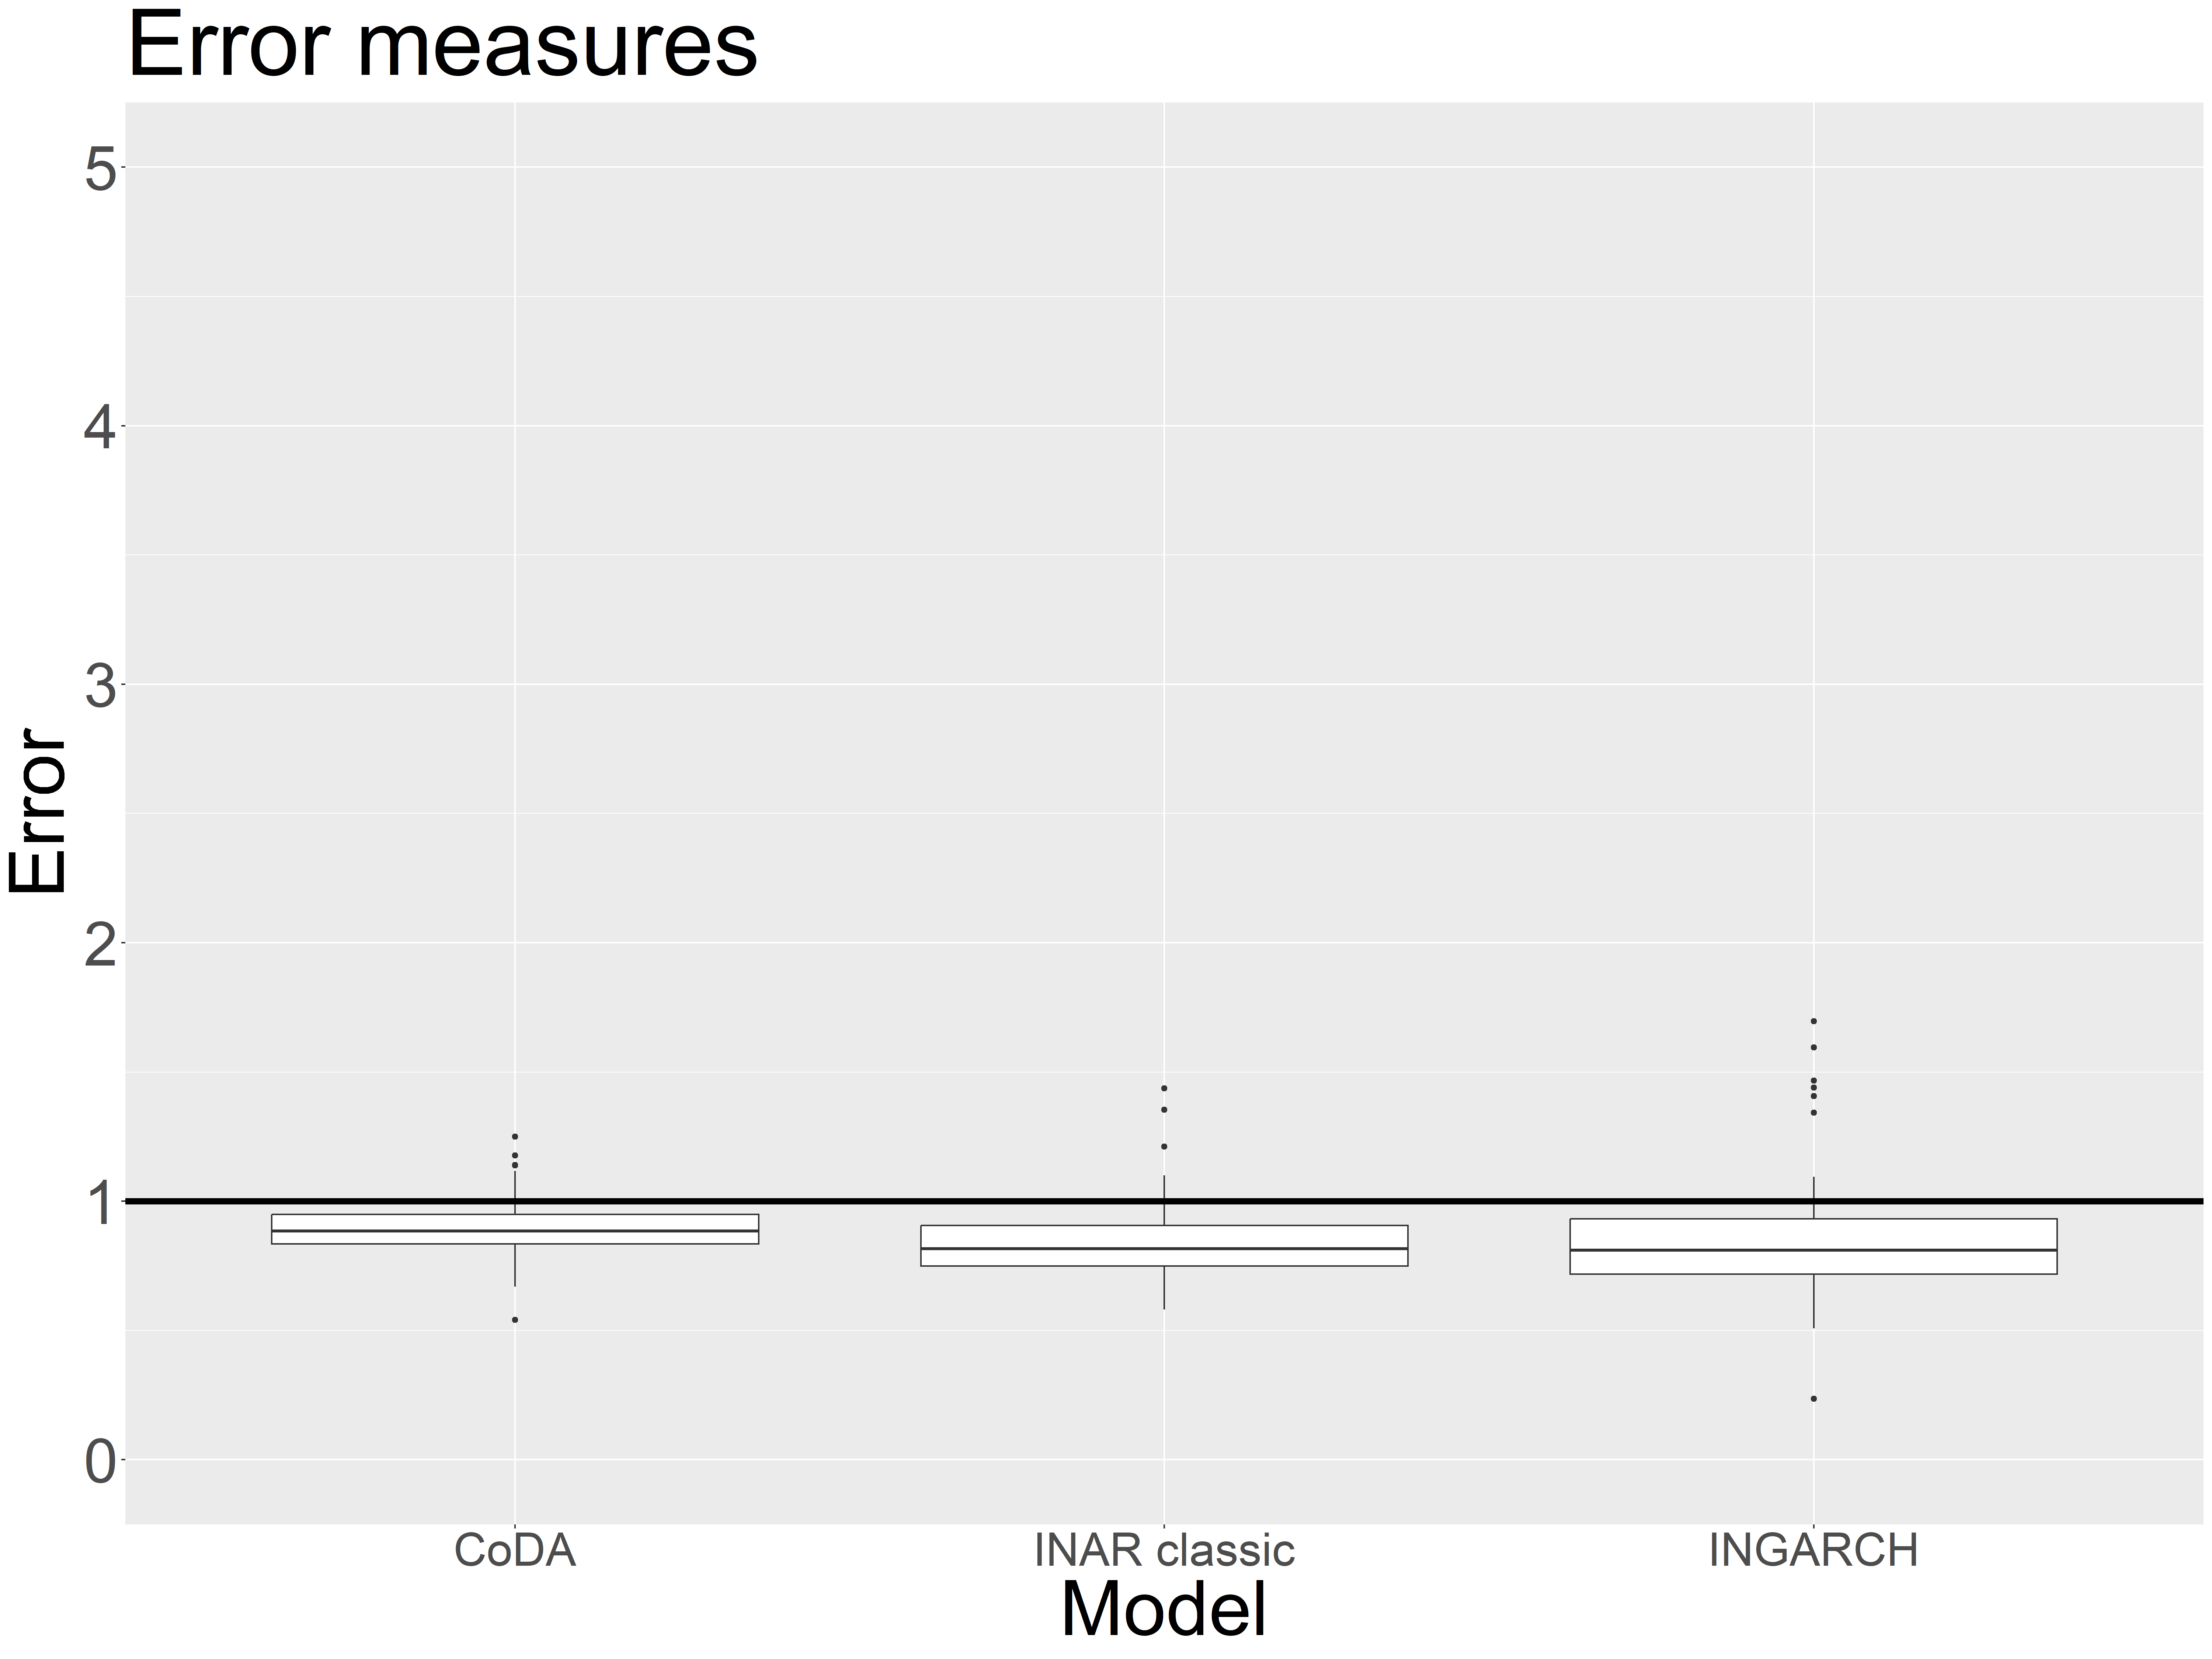
\includegraphics[width=\textwidth]{All_ErrorMeasure_combined_zoomed_ZIMFALSE.png}
\caption{Boxplot for the different models}
\label{fig:box distributions models}
\end{subfigure}
\hfill
\begin{subfigure}[b]{0.8\textwidth}
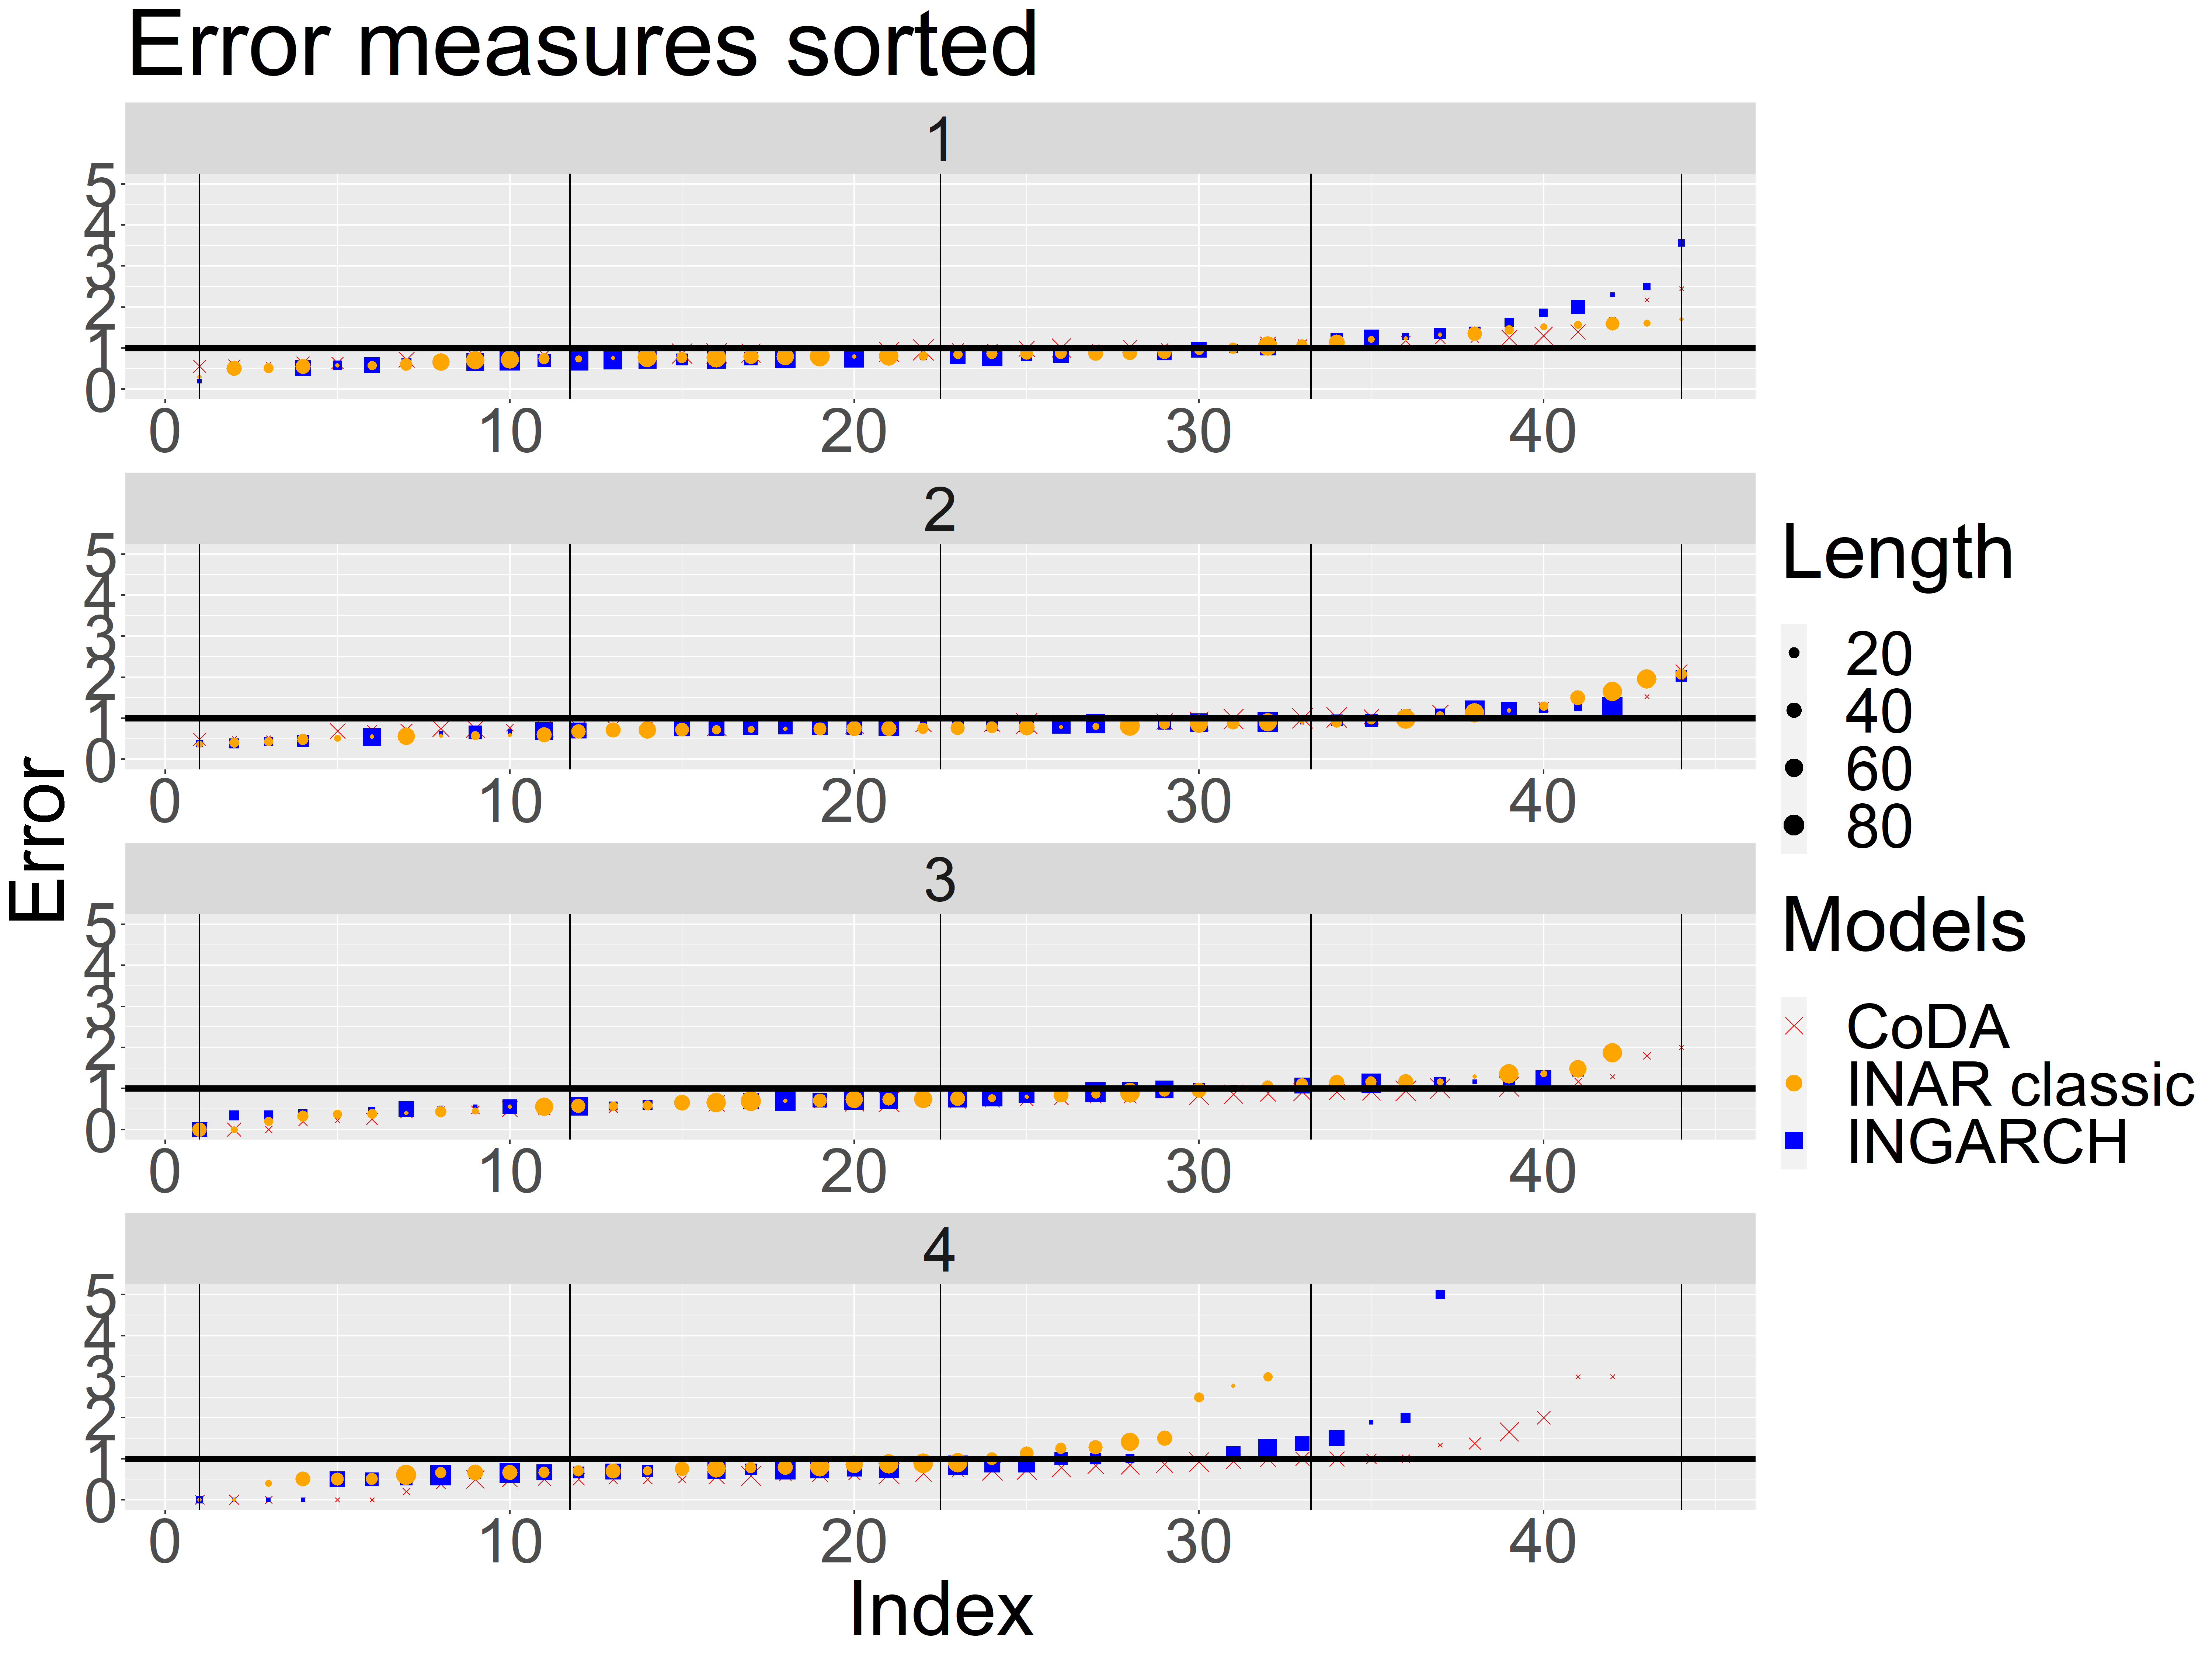
\includegraphics[width=\textwidth]{Quantile_Plot_Split_all_models_ZIMFALSE.png}
\caption{Quantiles for the different models}
\label{fig: quantile distributions models}
\end{subfigure}
\hfill
\caption{Comparison of the different models}
\label{fig:models Comp1}
\end{figure}

In figure \ref{fig:models Comp2} we also include the ZIM model. One drawback about the ZIM model is, that it needs to have zero values in the fitted window. Because of the lack of them in category 1 and 2, we couldn't manage to fit it. Hence the models in \ref{fig:models Comp2} were only fitted on categories 3 and 4. 

In \ref{fig:box distributions models Zim} we again see the boxplot for the summarised error. The ZIM and CoDA model exhibit similar performance and both are slightly worse than the INAR and INGARCH model. In \ref{fig: quantile distributions models Zim} we see again the error measure for each category. While the models perform similar for category 3, the ZIM and INGARCH model outperform the INAR and CoDA model for category 4. Here it is worth mentioning, that category 4 is the main category with the most amount of zeros in our data. Especially CoDA seems to struggle with the big amount of zeros present. 

\begin{figure}[htb!]
\centering
\begin{subfigure}[b]{0.8\textwidth}
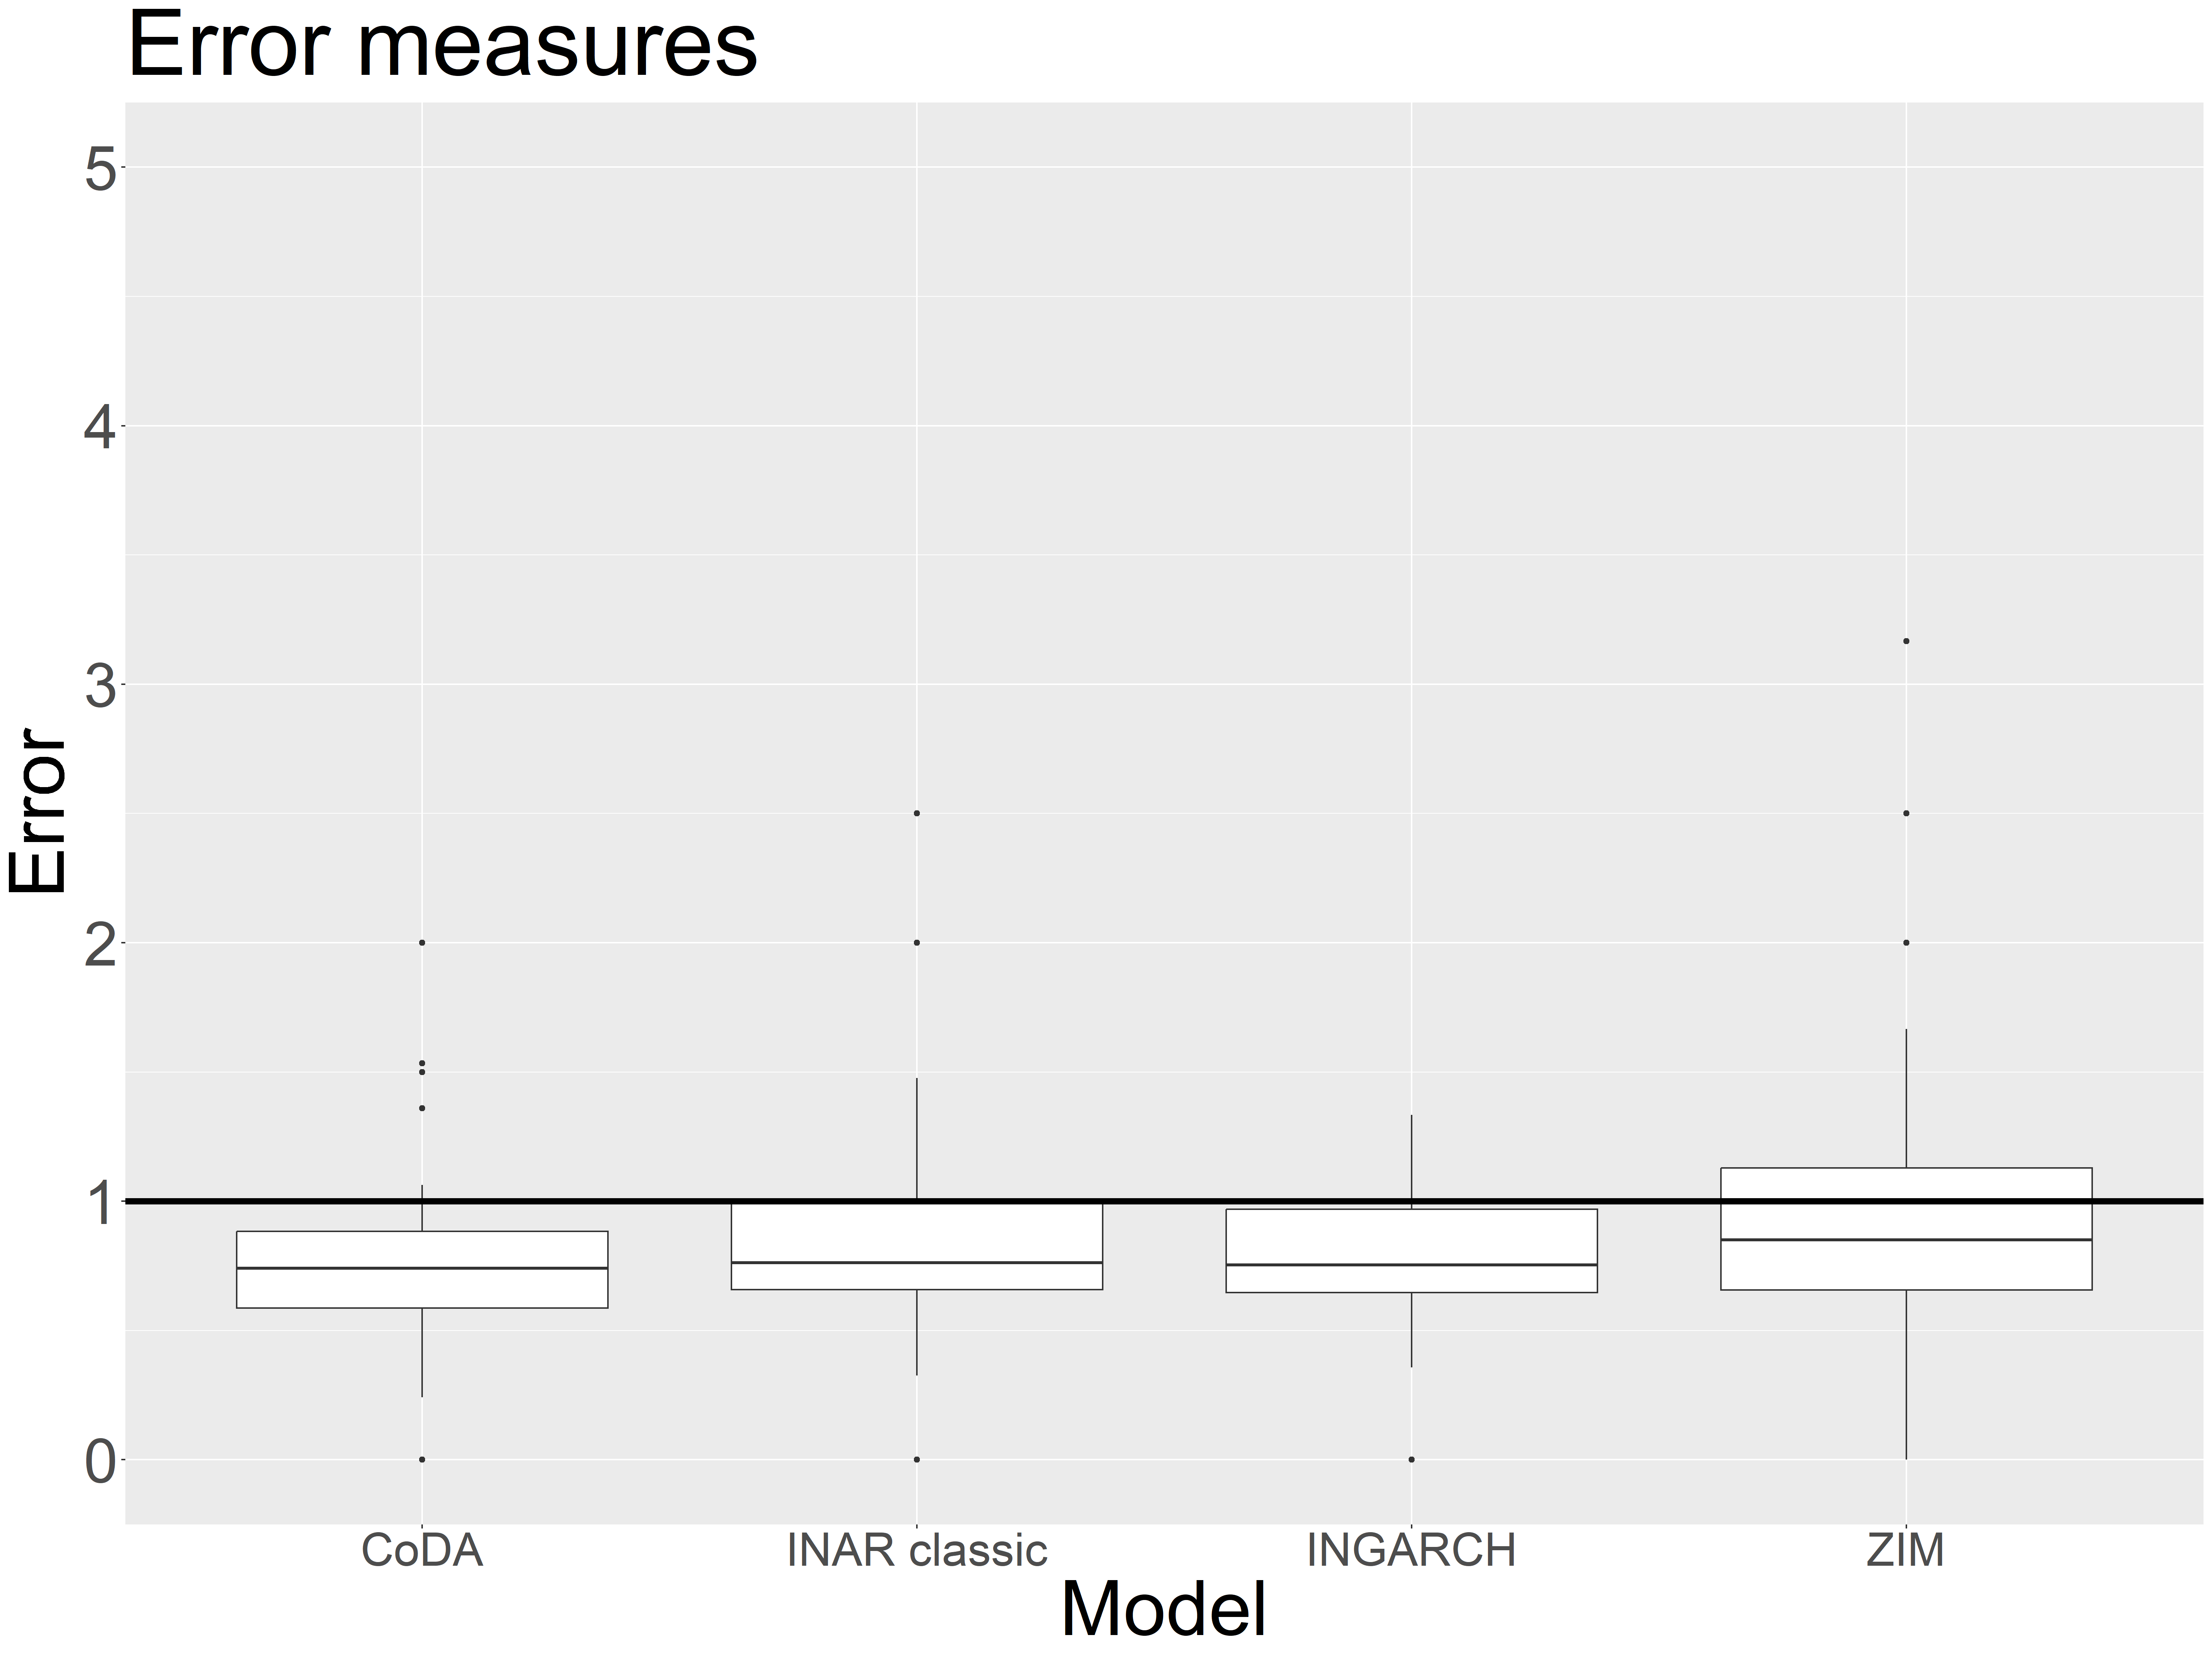
\includegraphics[width=\textwidth]{All_ErrorMeasure_combined_zoomed_ZIMTRUE.png}
\caption{Boxplot for the different models}
\label{fig:box distributions models Zim}
\end{subfigure}
\hfill
\begin{subfigure}[b]{0.8\textwidth}
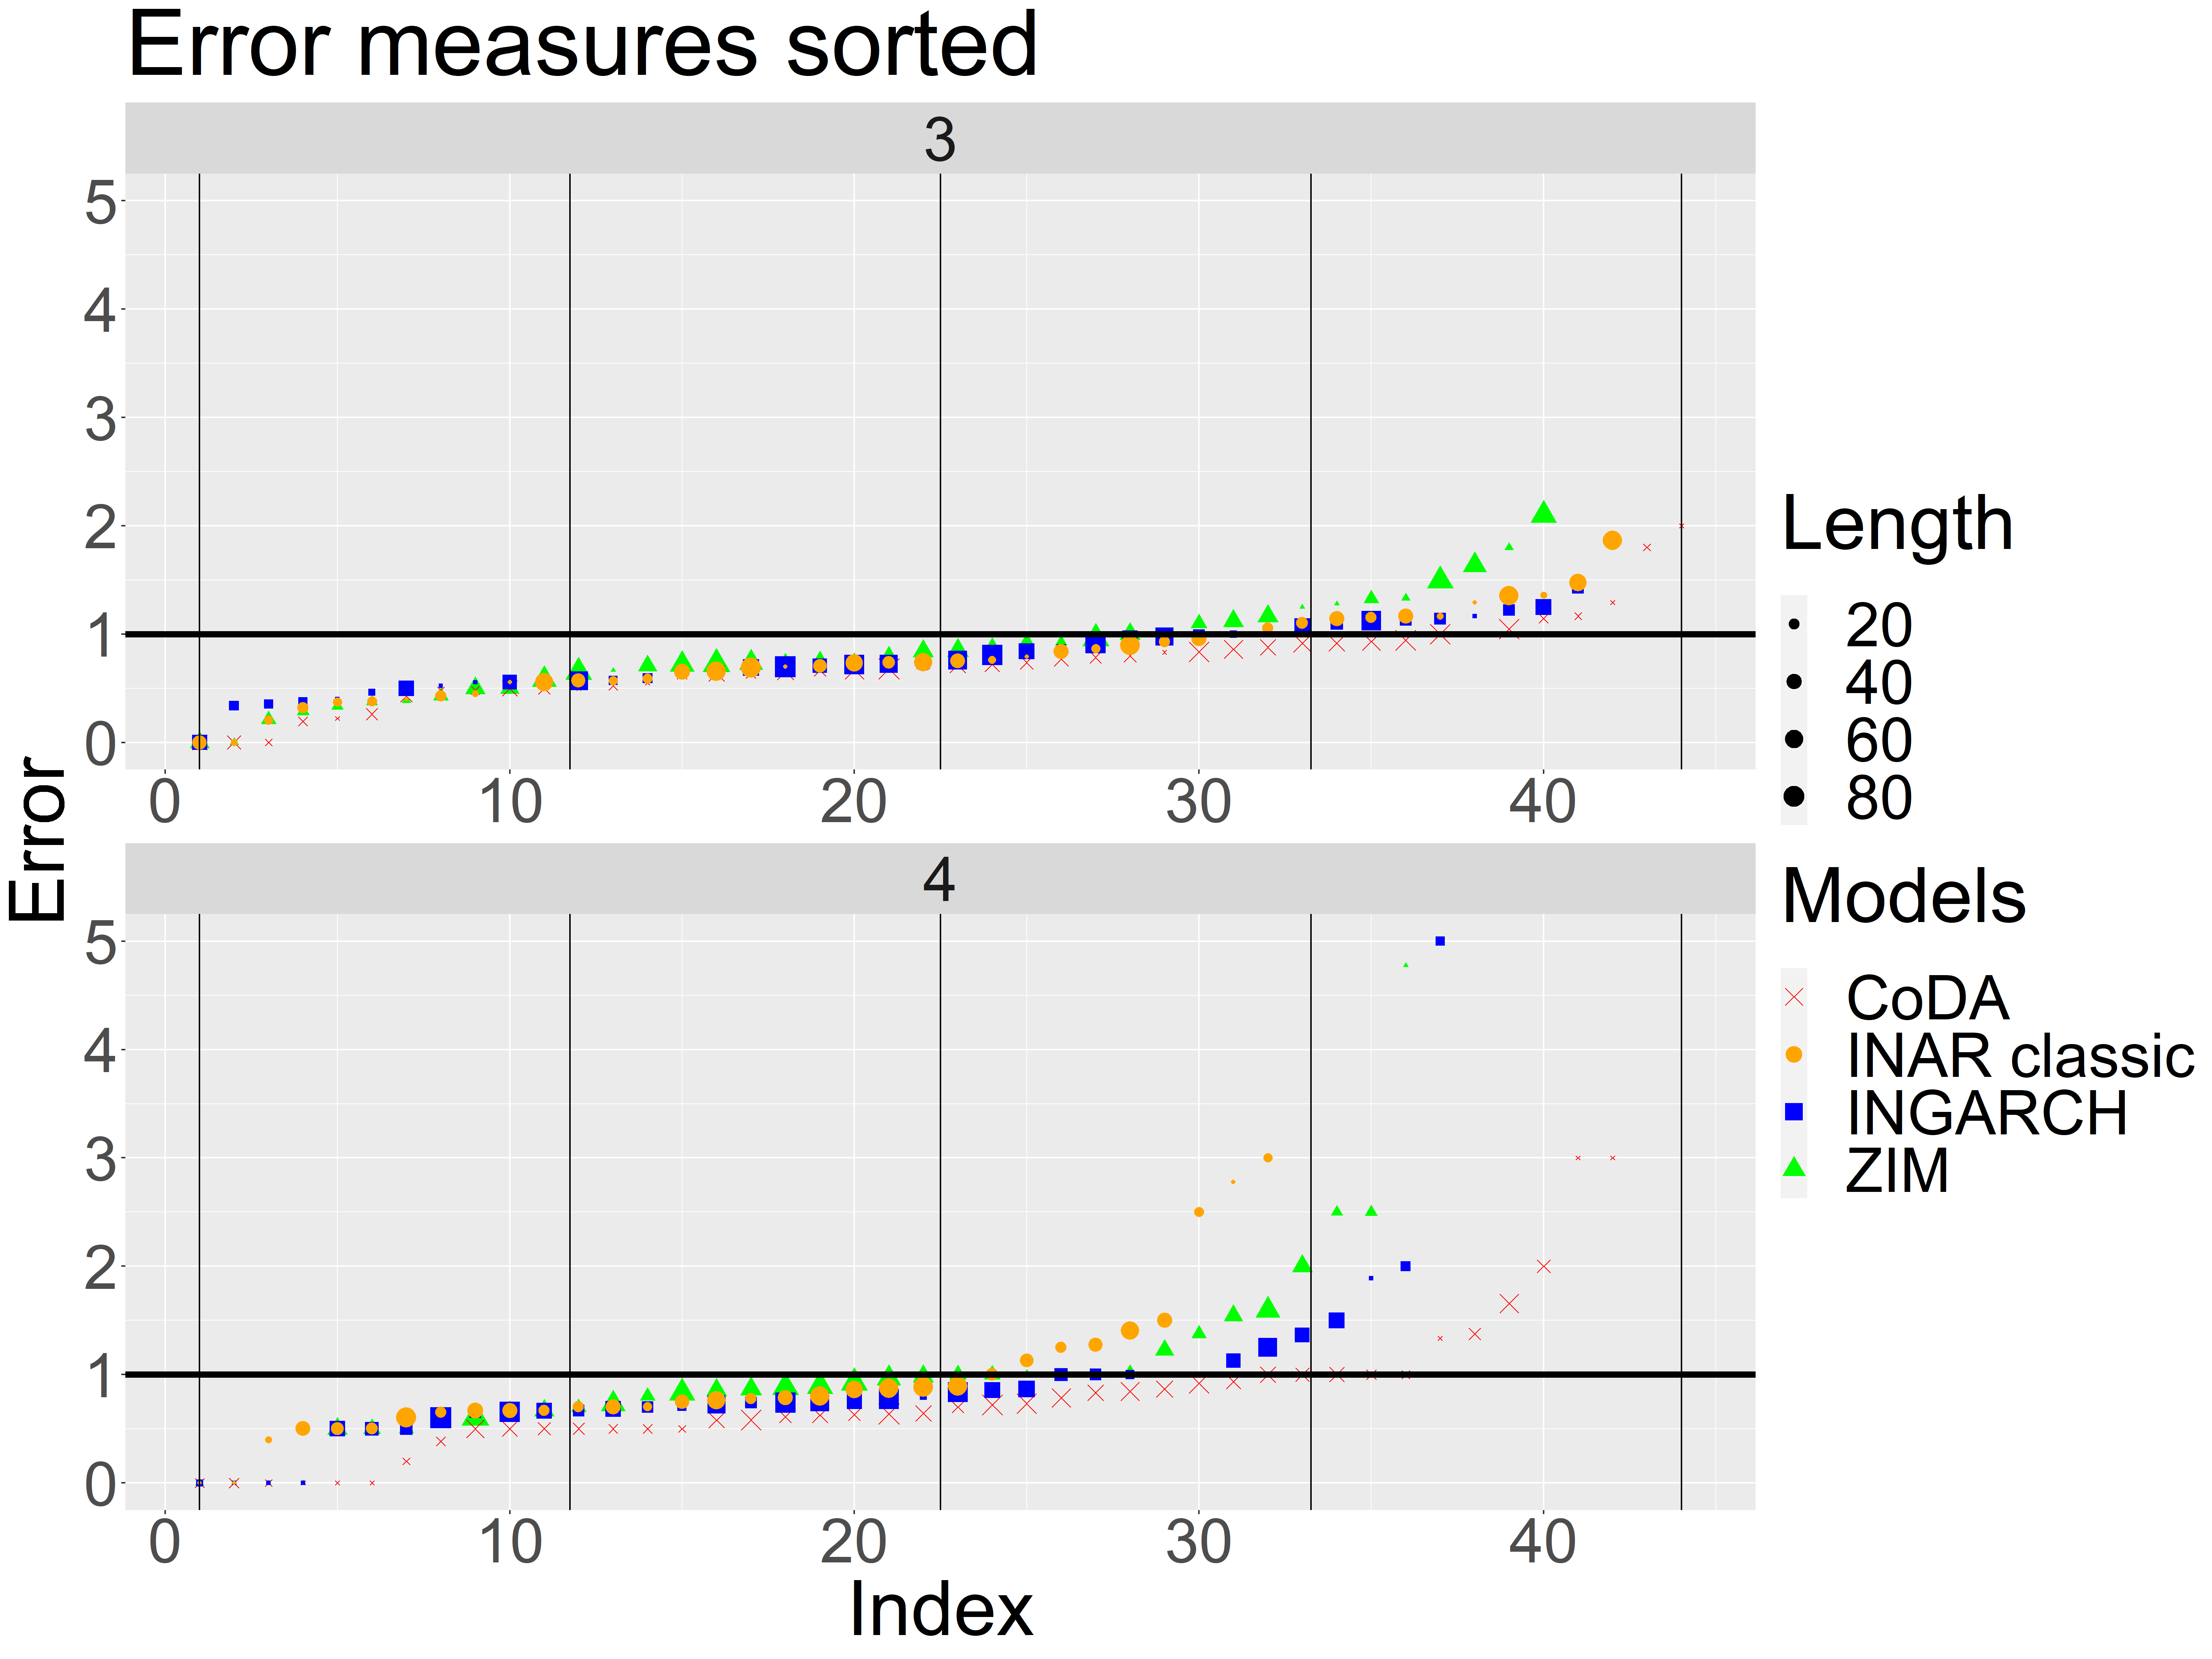
\includegraphics[width=\textwidth]{Quantile_Plot_Split_all_models_ZIMTRUE.png}
\caption{Quantiles for the different models}
\label{fig: quantile distributions models Zim}
\end{subfigure}
\hfill
\caption{Comparison of the different models }
\label{fig:models Comp2}
\end{figure}



\subsection{General Specifications}
\label{sec:General Specifications}

First, we start with specifications which can be chosen for both CoDA and INGARCH. We will always vary one parameter, while using the respective standard values for the other parameters. 
\subsubsection{History}
\label{sec:History}

As mentioned various times throughout this thesis, the the history is one of the parameters which can be adjusted. In figure \ref{fig:History Comp1} we visualise the results as a boxplot, a quantile plot as before and additionally an histogram to get a feeling for the error distribution. 

\begin{figure}[htb!]
\centering
\begin{subfigure}[b]{0.45\textwidth}
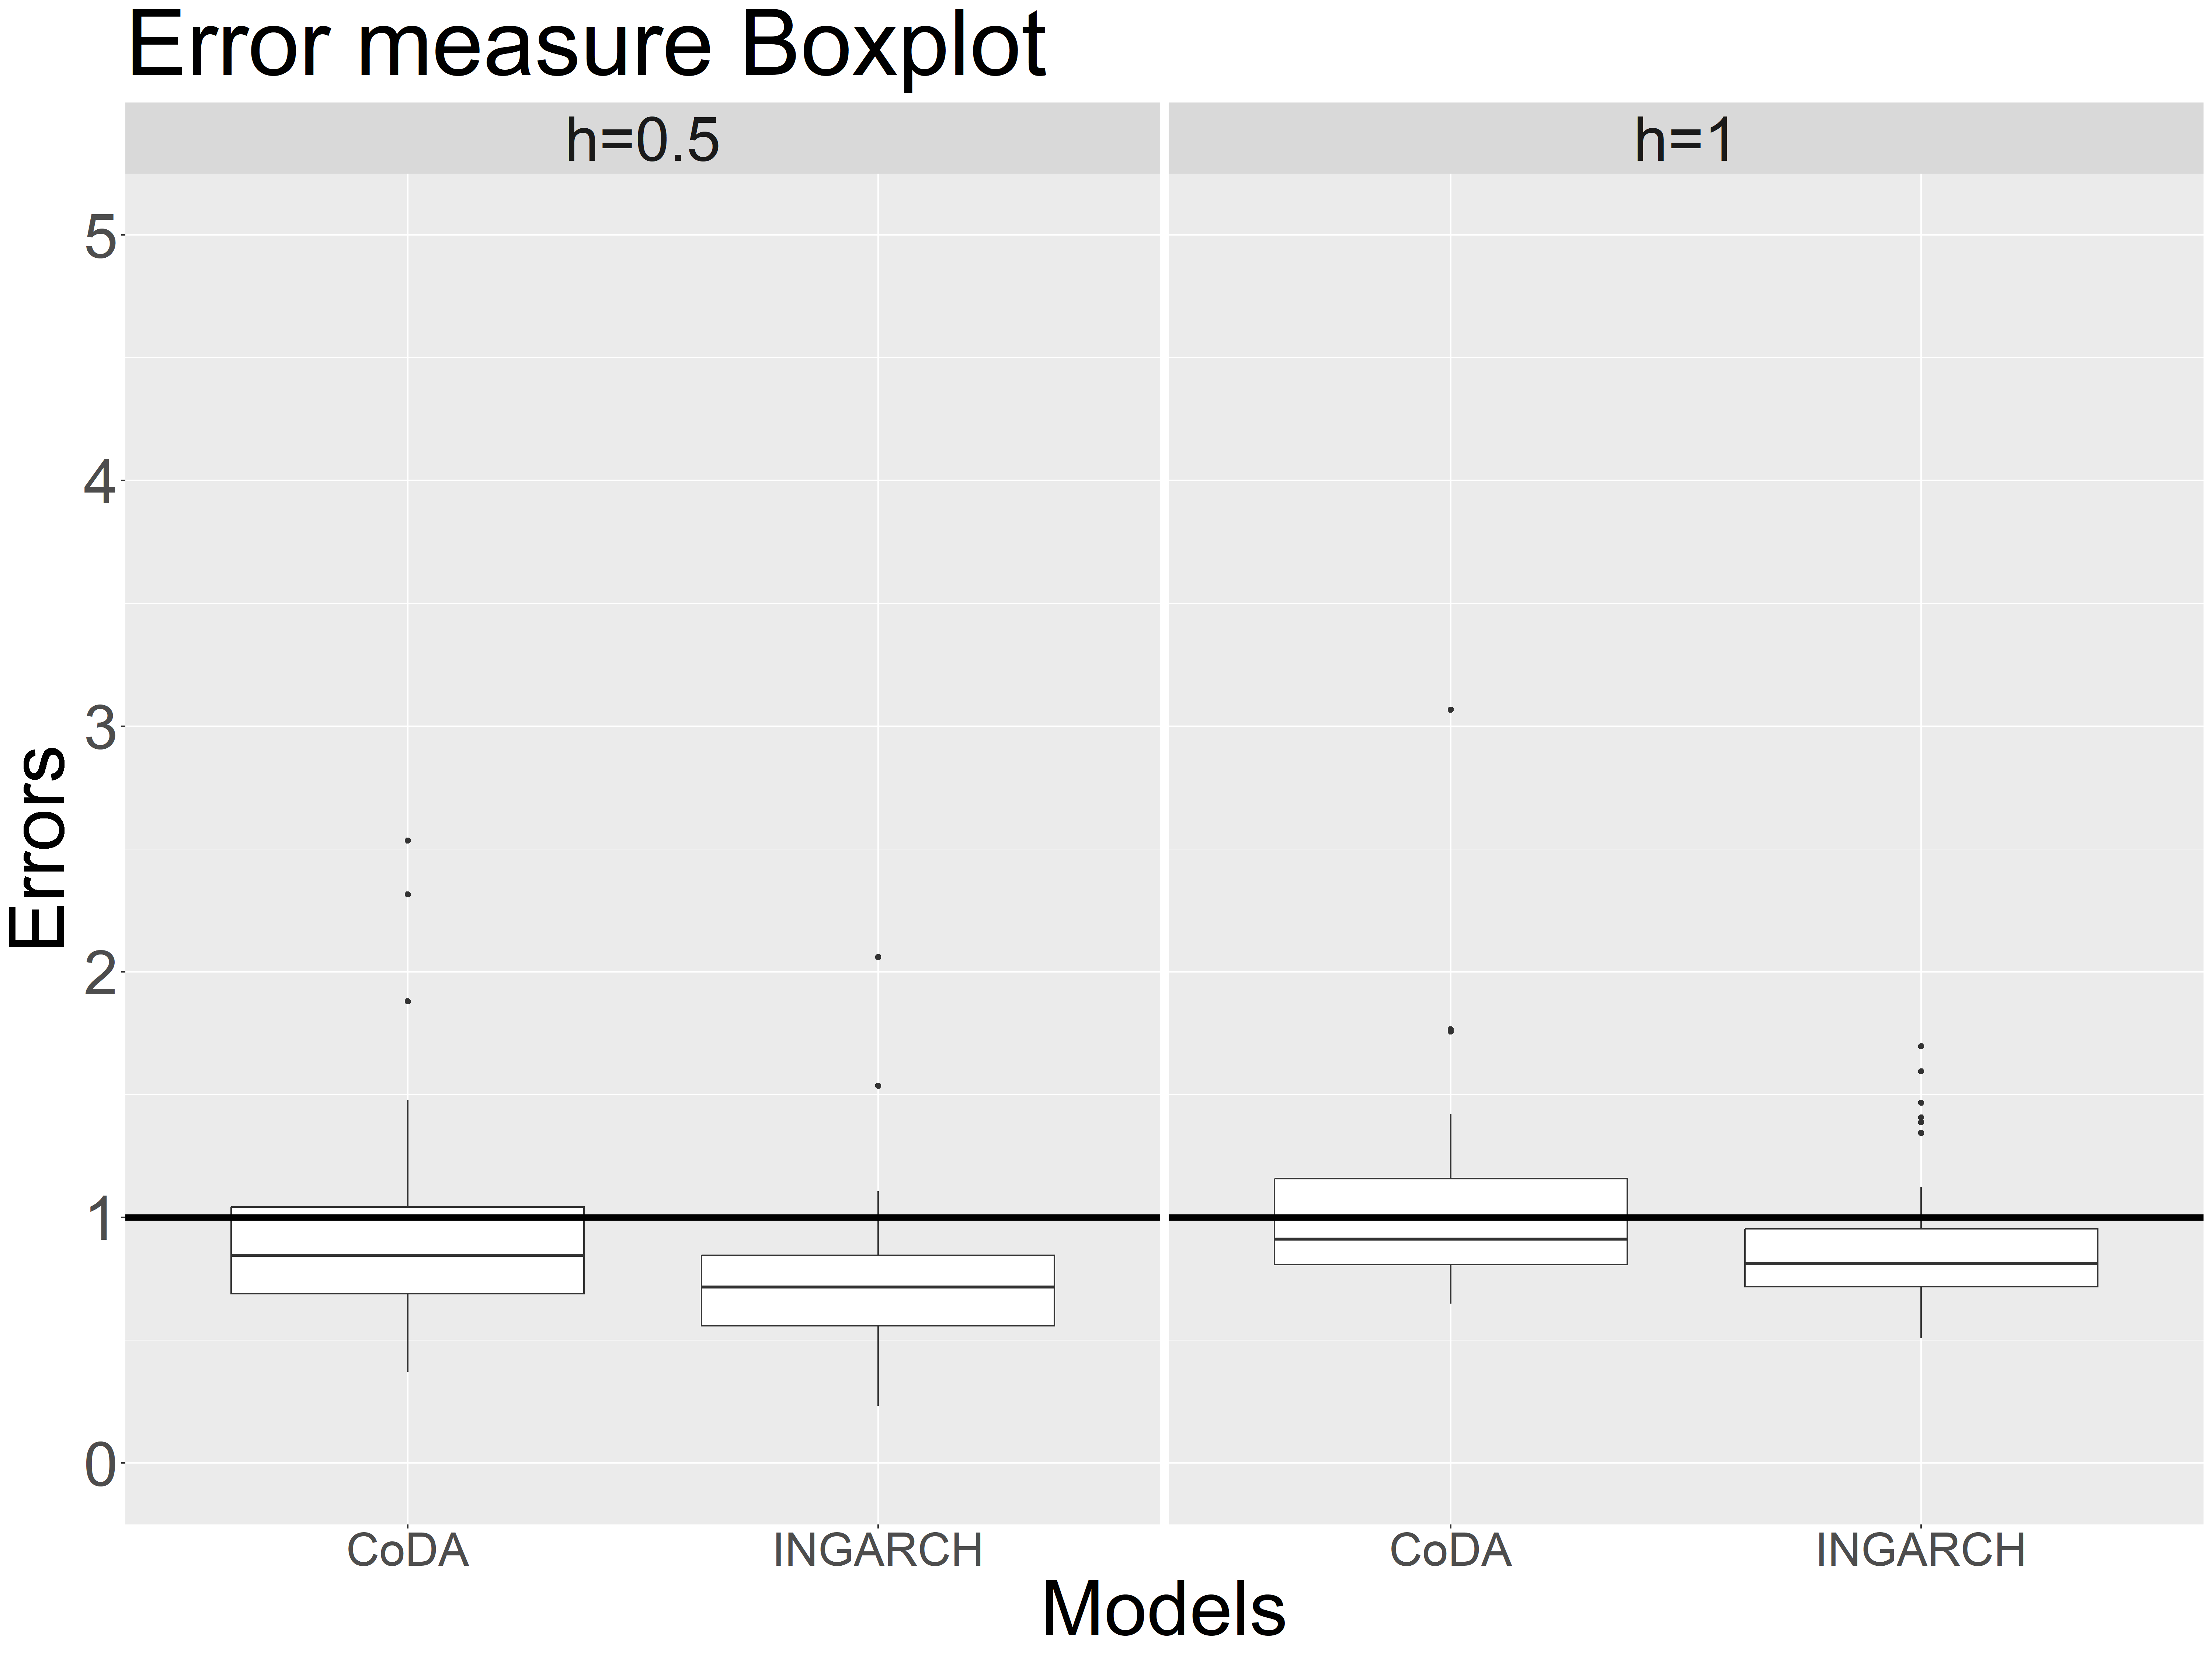
\includegraphics[width=\textwidth]{ErrorMeasureCombined_Box_all__Variation_history.png}
\caption{Boxplot of different $h$}
\label{fig:History Box}
\end{subfigure}
\hfill
\begin{subfigure}[b]{0.45\textwidth}
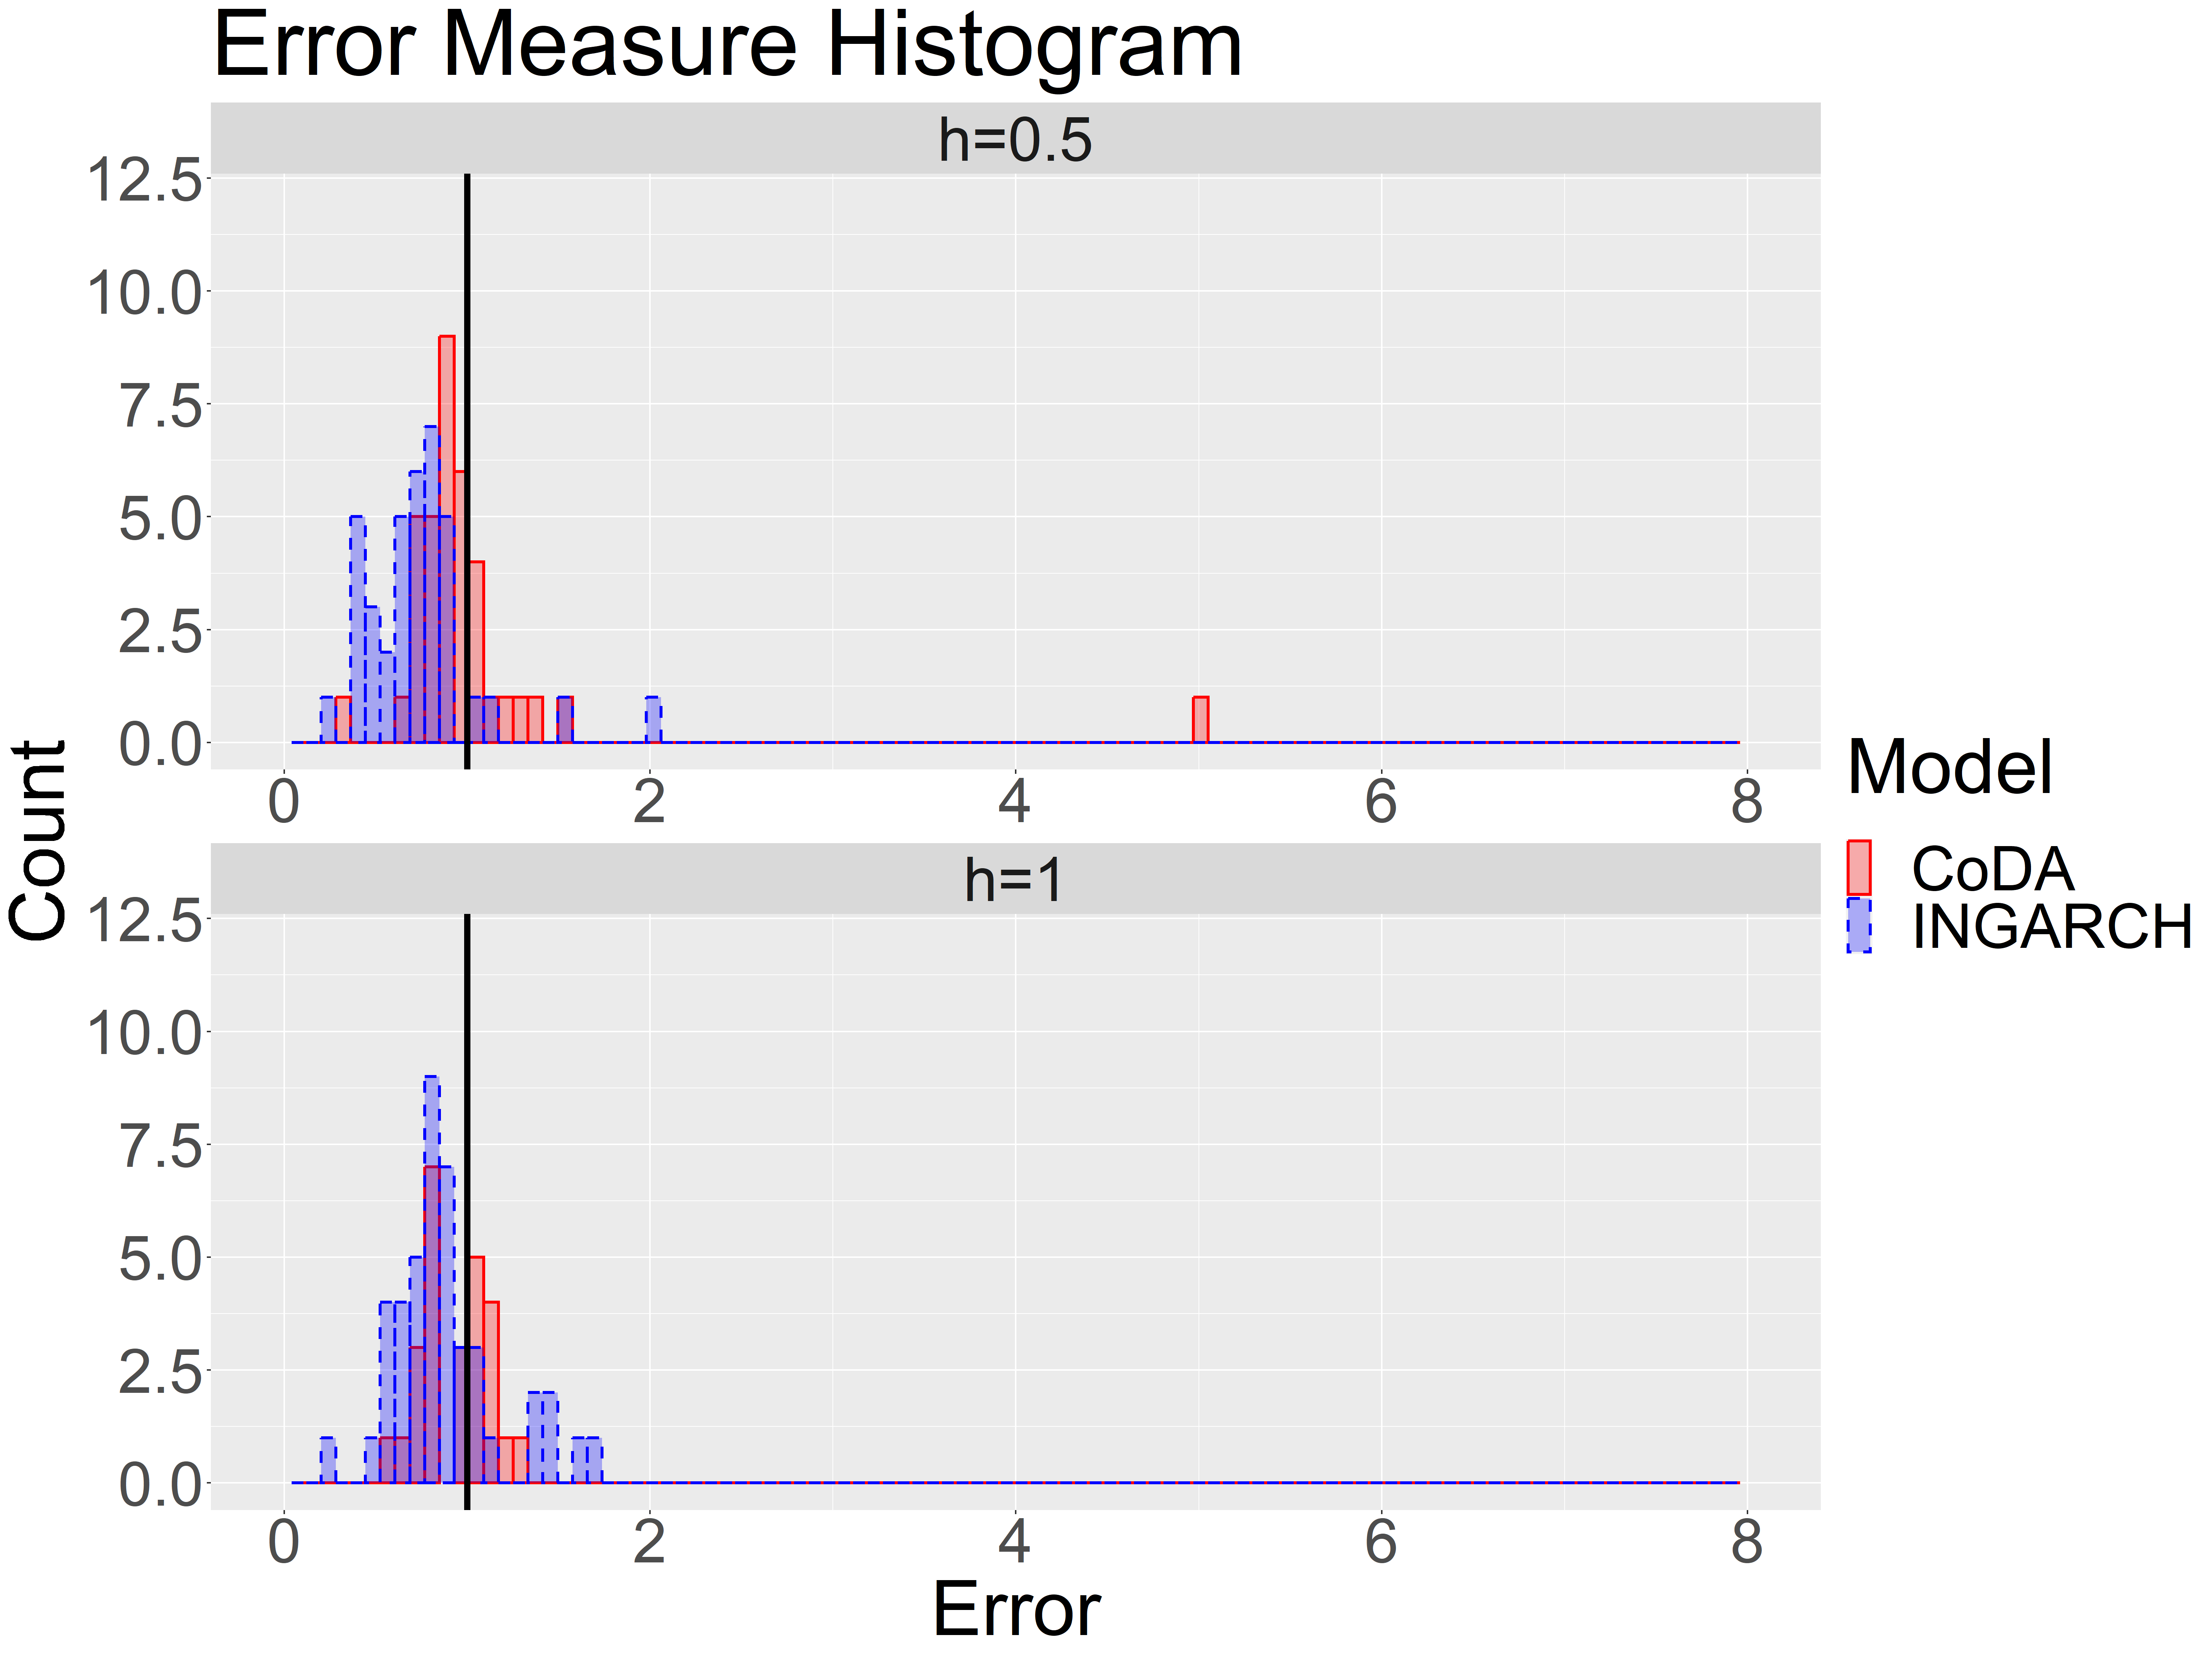
\includegraphics[width=\textwidth]{ErrorMeasureCombined_Histogram_all__Variation_history.png}
\caption{Histogram of different $h$}
\label{fig:History Hist}
\end{subfigure}
\hfill
\begin{subfigure}[b]{0.8\textwidth}
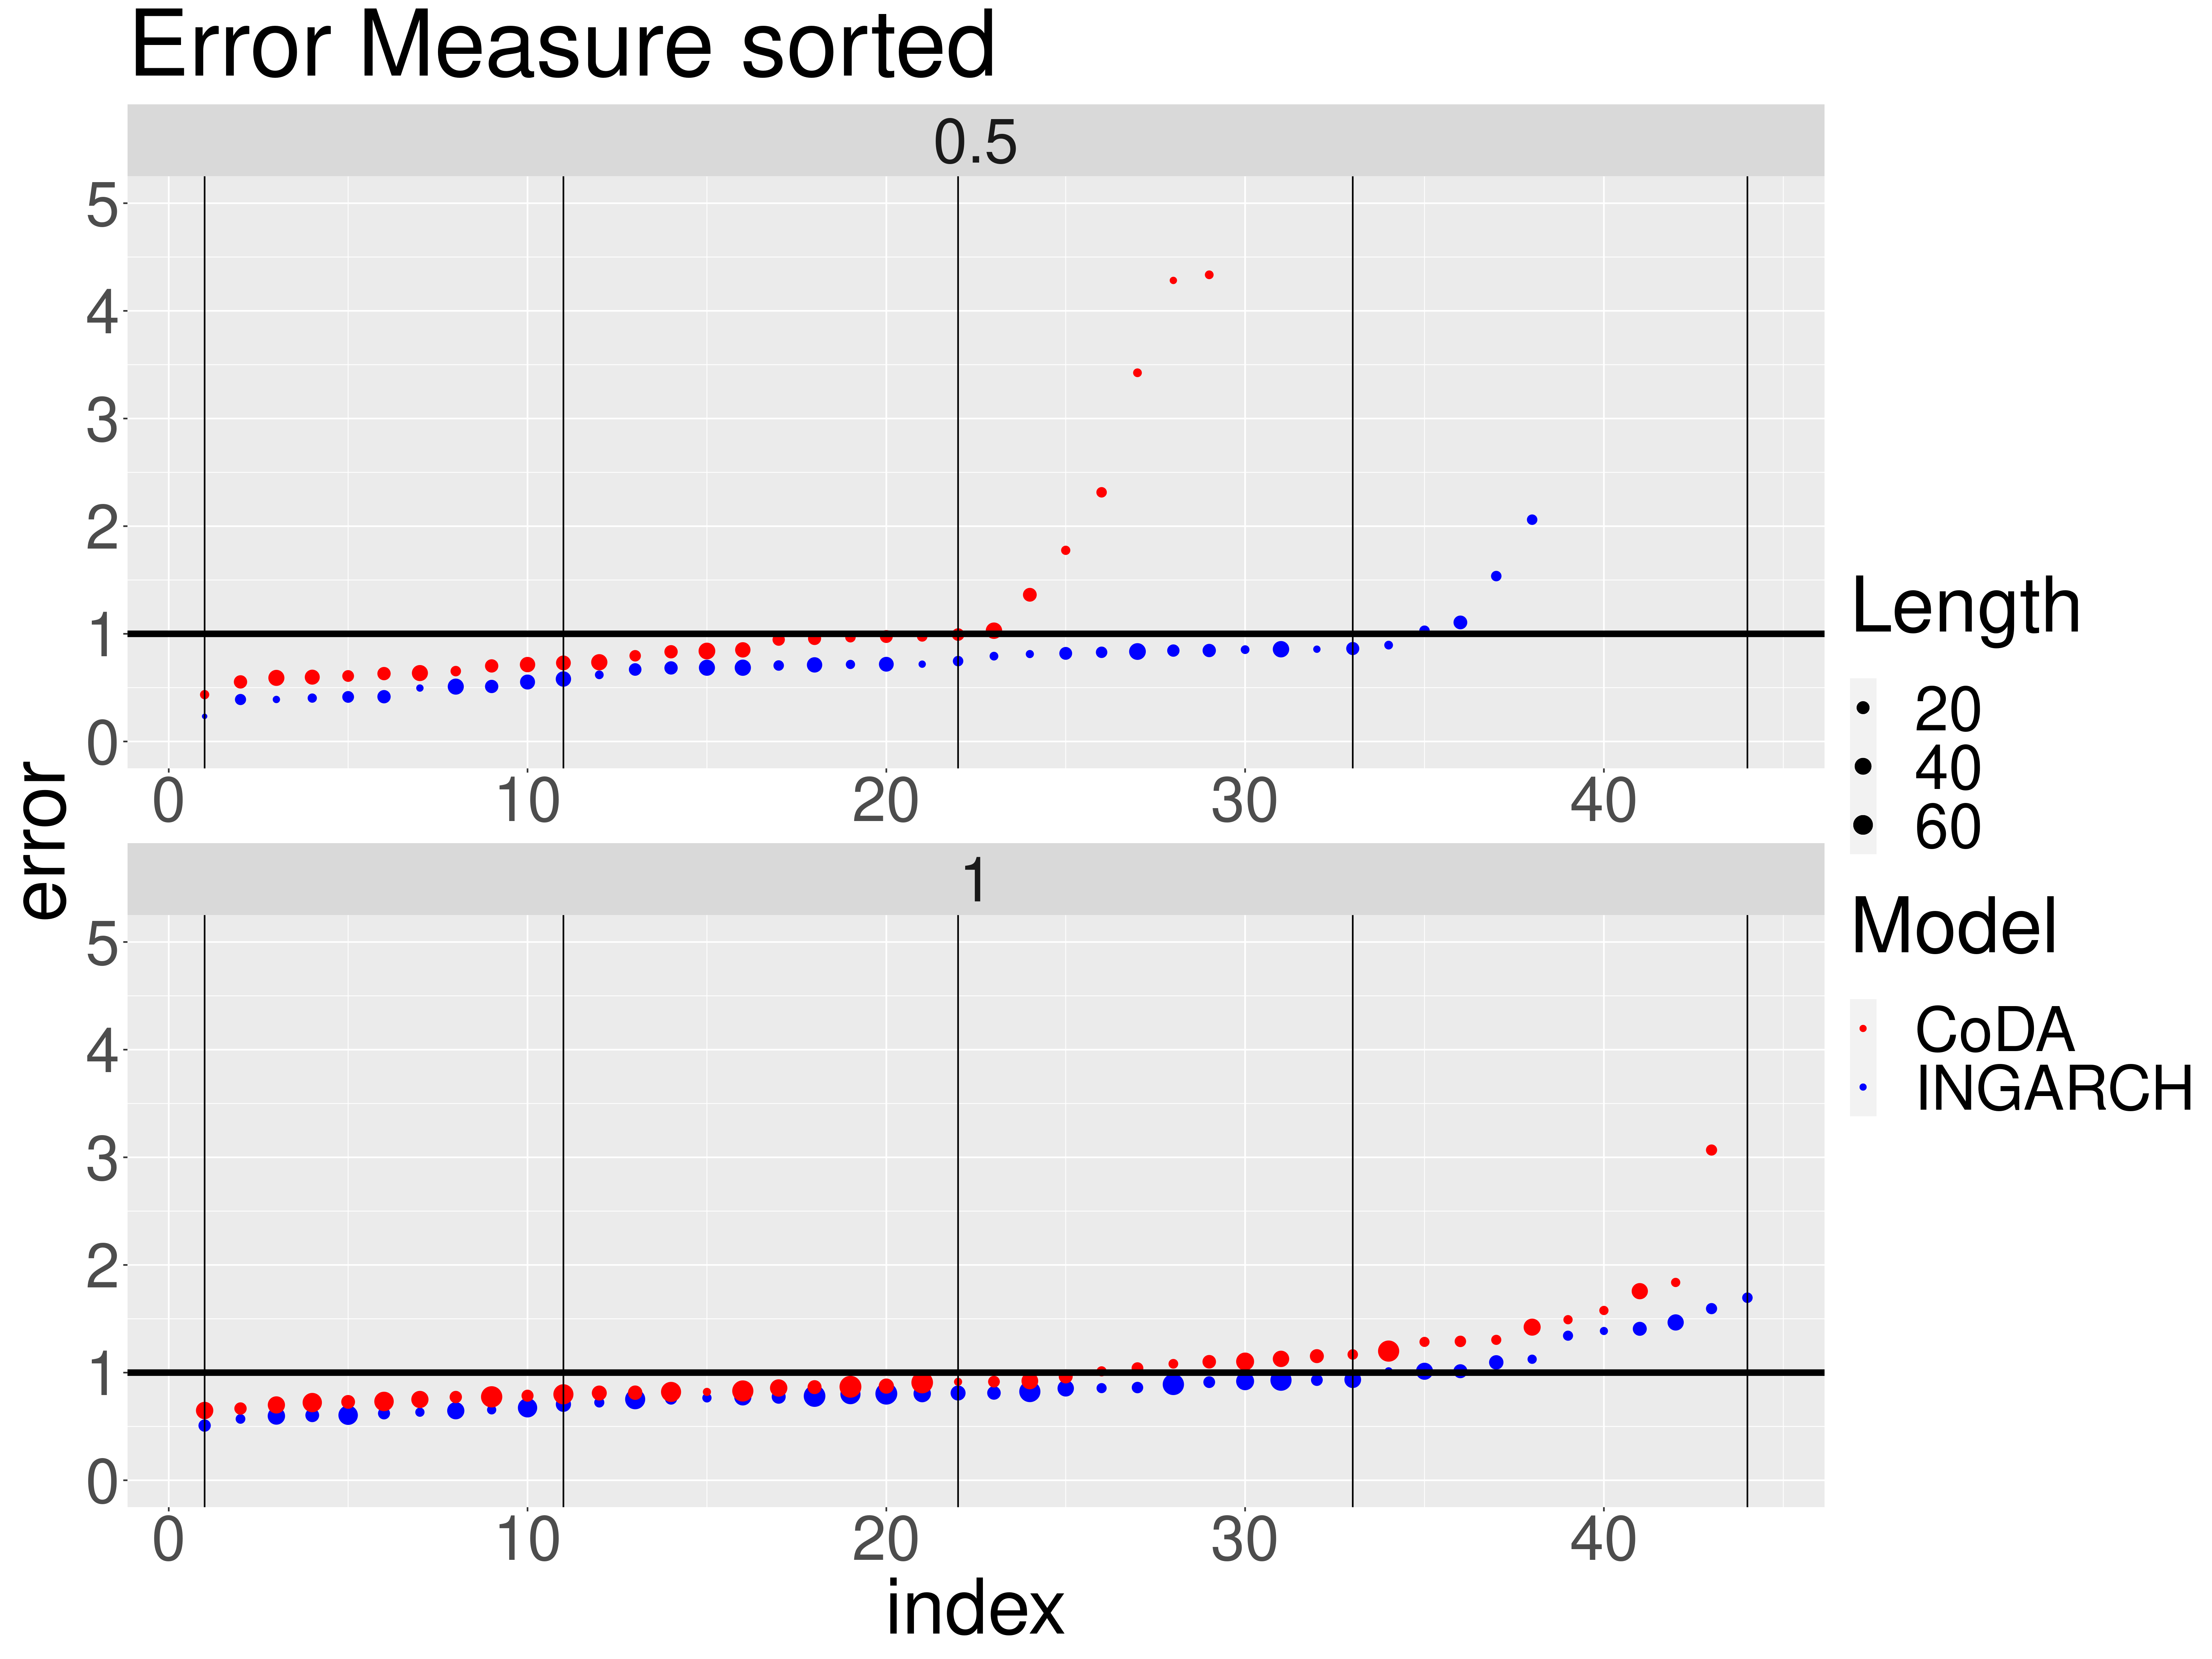
\includegraphics[width=\textwidth]{ErrorMeasureCombined_Quant_all__Variation_history.png}
\caption{Quantiles Plot of different $h$}
\label{fig:History Quant}
\end{subfigure}
\caption{Comparison of different $h$}
\label{fig:History Comp1}
\end{figure}

In figure \ref{fig:History Comp1} we can see that the results for CoDA does not vary too much for the different histories. However, one can see in the quantile plot \ref{fig:History Quant} that we have 8 less values for  $h=0.5$ than for $h=1$. This probably results from the fact, that if we only take half of the history for an already short time series, that we have too little values for estimating. 

For INGARCH, the results are similar as well. For $h=1$ we get slightly higher values for the error measure as seen in \ref{fig:History Box}. But again in \ref{fig:History Quant} we see that we have less values for the shorter history for the same reason as above. 

\subsubsection{Frame}
\label{sec:Frame}

Next, we vary the initial frame length $w_f$. We choose to extend the frame with each new data point. For this we vary the value $w$ in $w_f=w\cdot T$. The results are portrayed in \ref{fig:Frame Comp1}. In general, there is not much difference between the different frames. INGARCH seems to perform better for all three values.
\begin{figure}[htb!]
\centering
\begin{subfigure}[b]{0.45\textwidth}
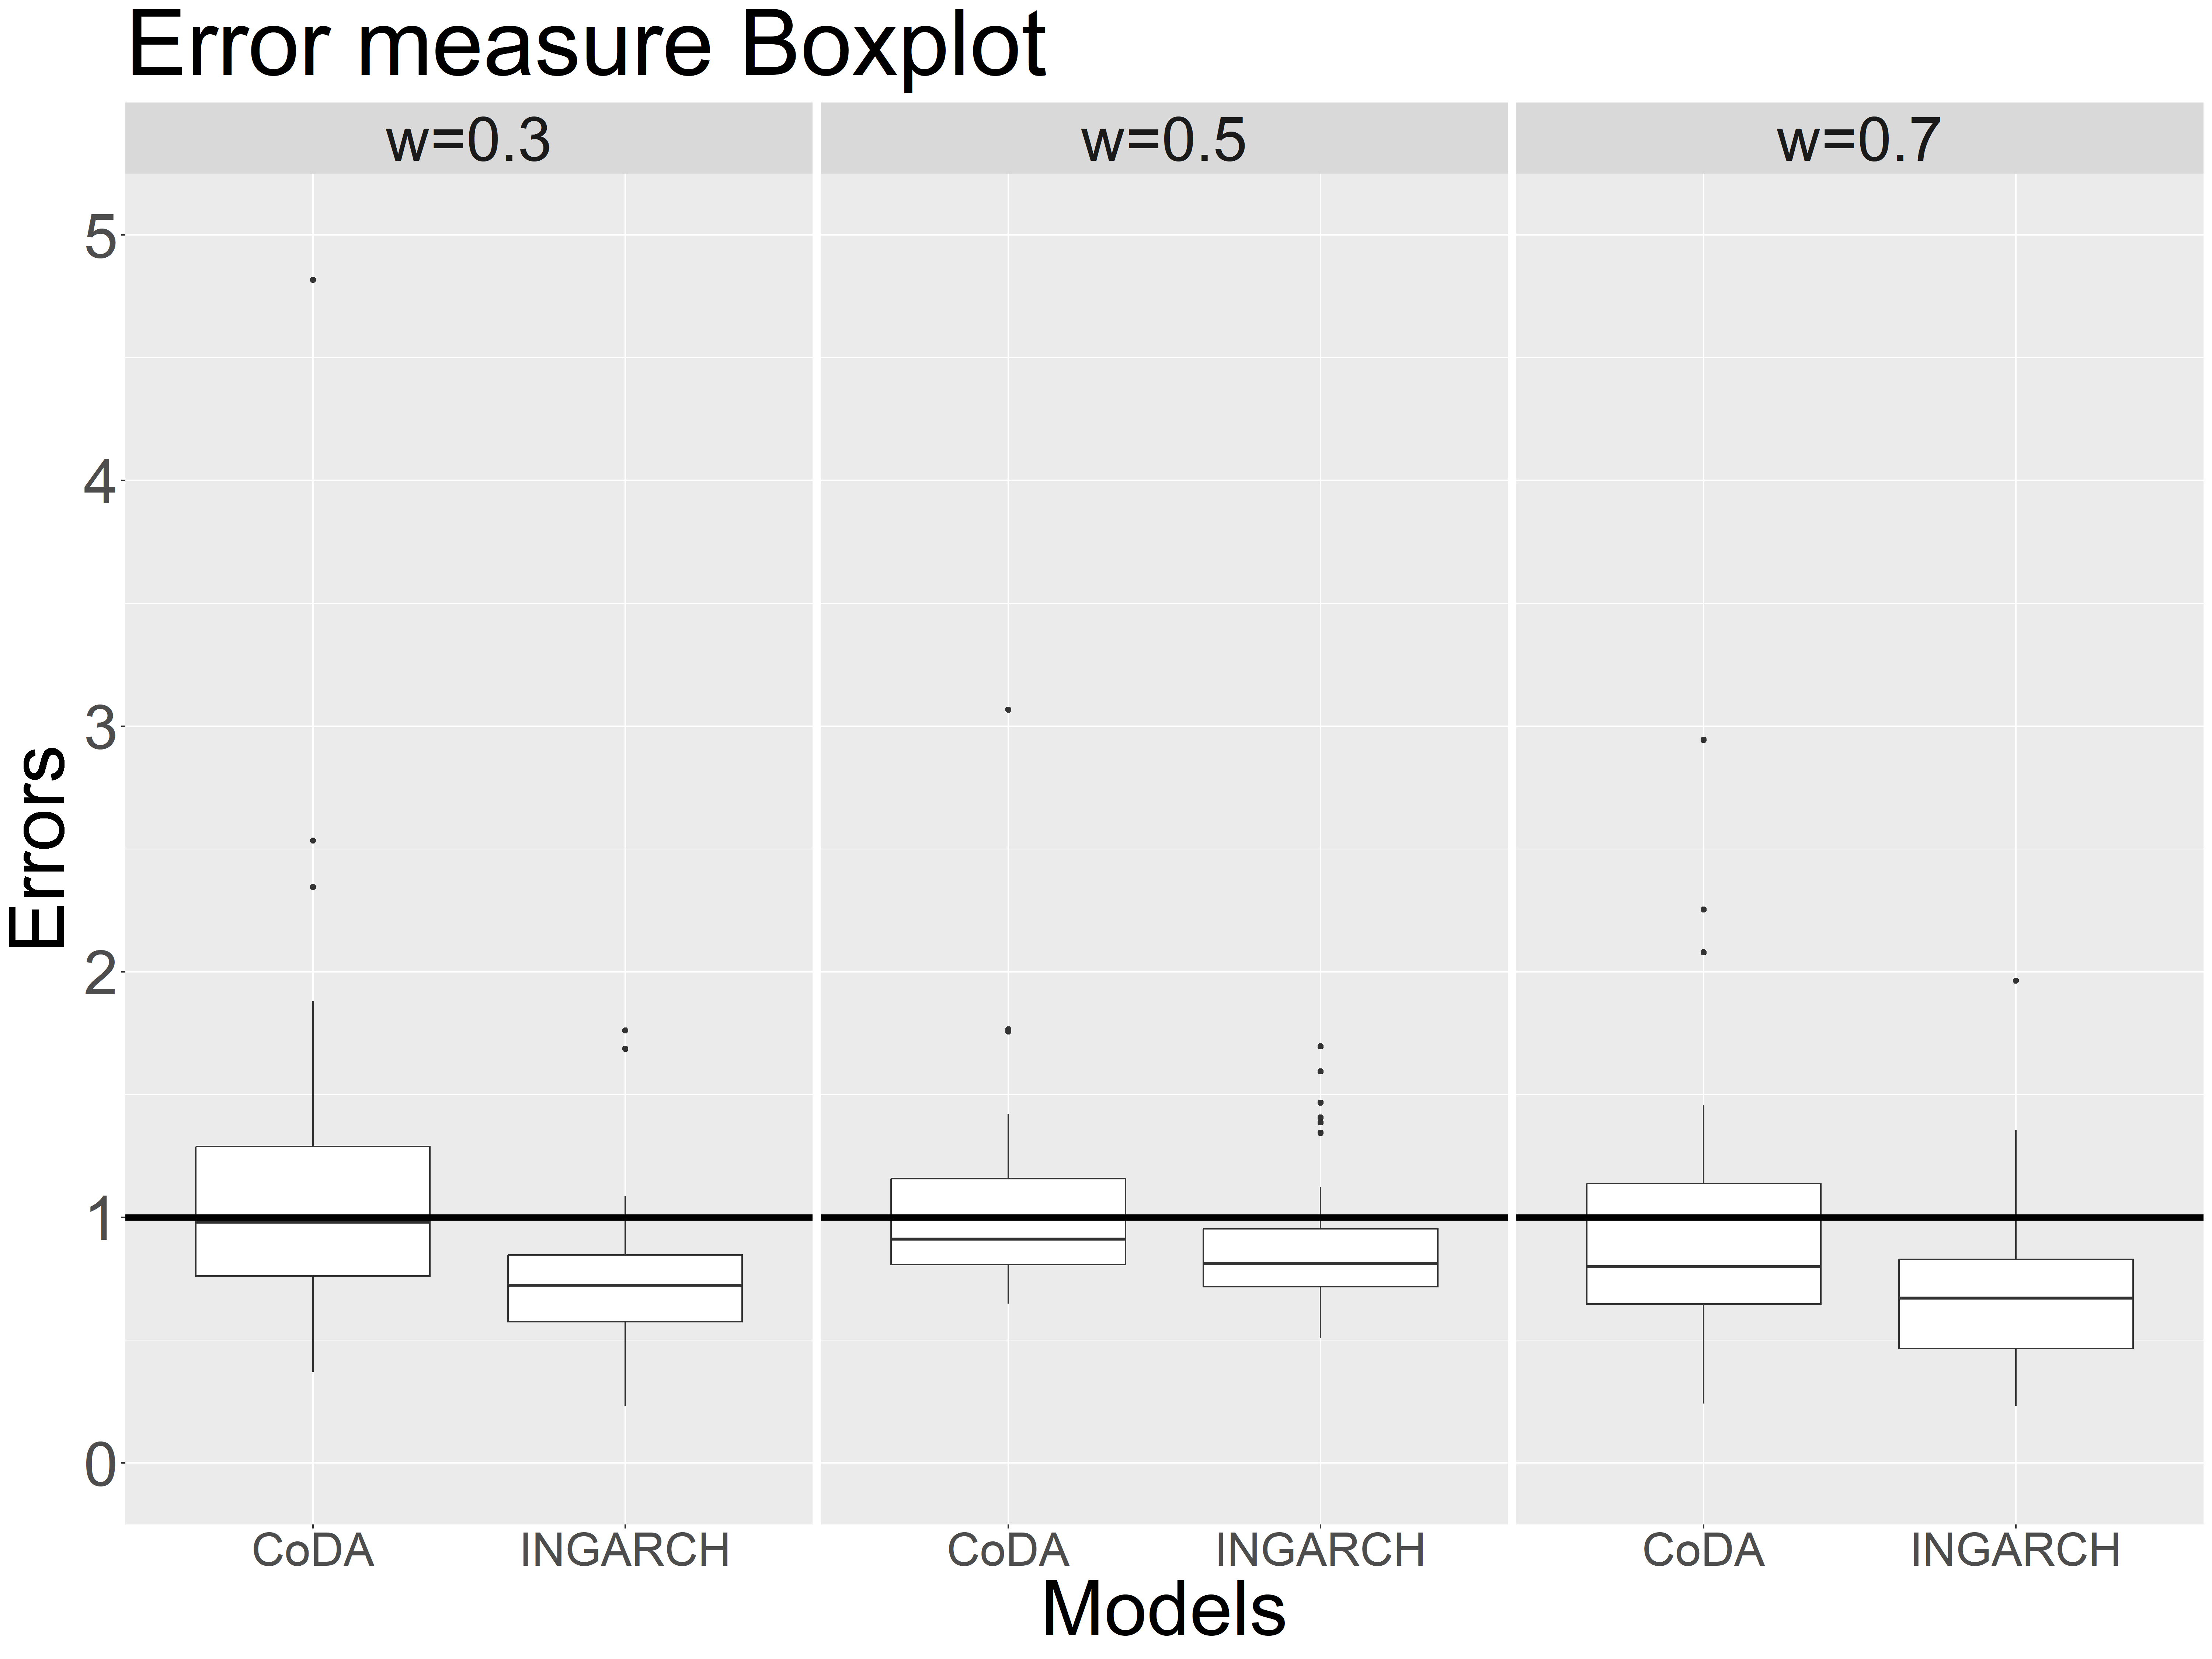
\includegraphics[width=\textwidth]{ErrorMeasureCombined_Box_all__Variation_frame.png}
\caption{Boxplot of different $w$}
\label{fig:Frame Box}
\end{subfigure}
\hfill
\begin{subfigure}[b]{0.45\textwidth}
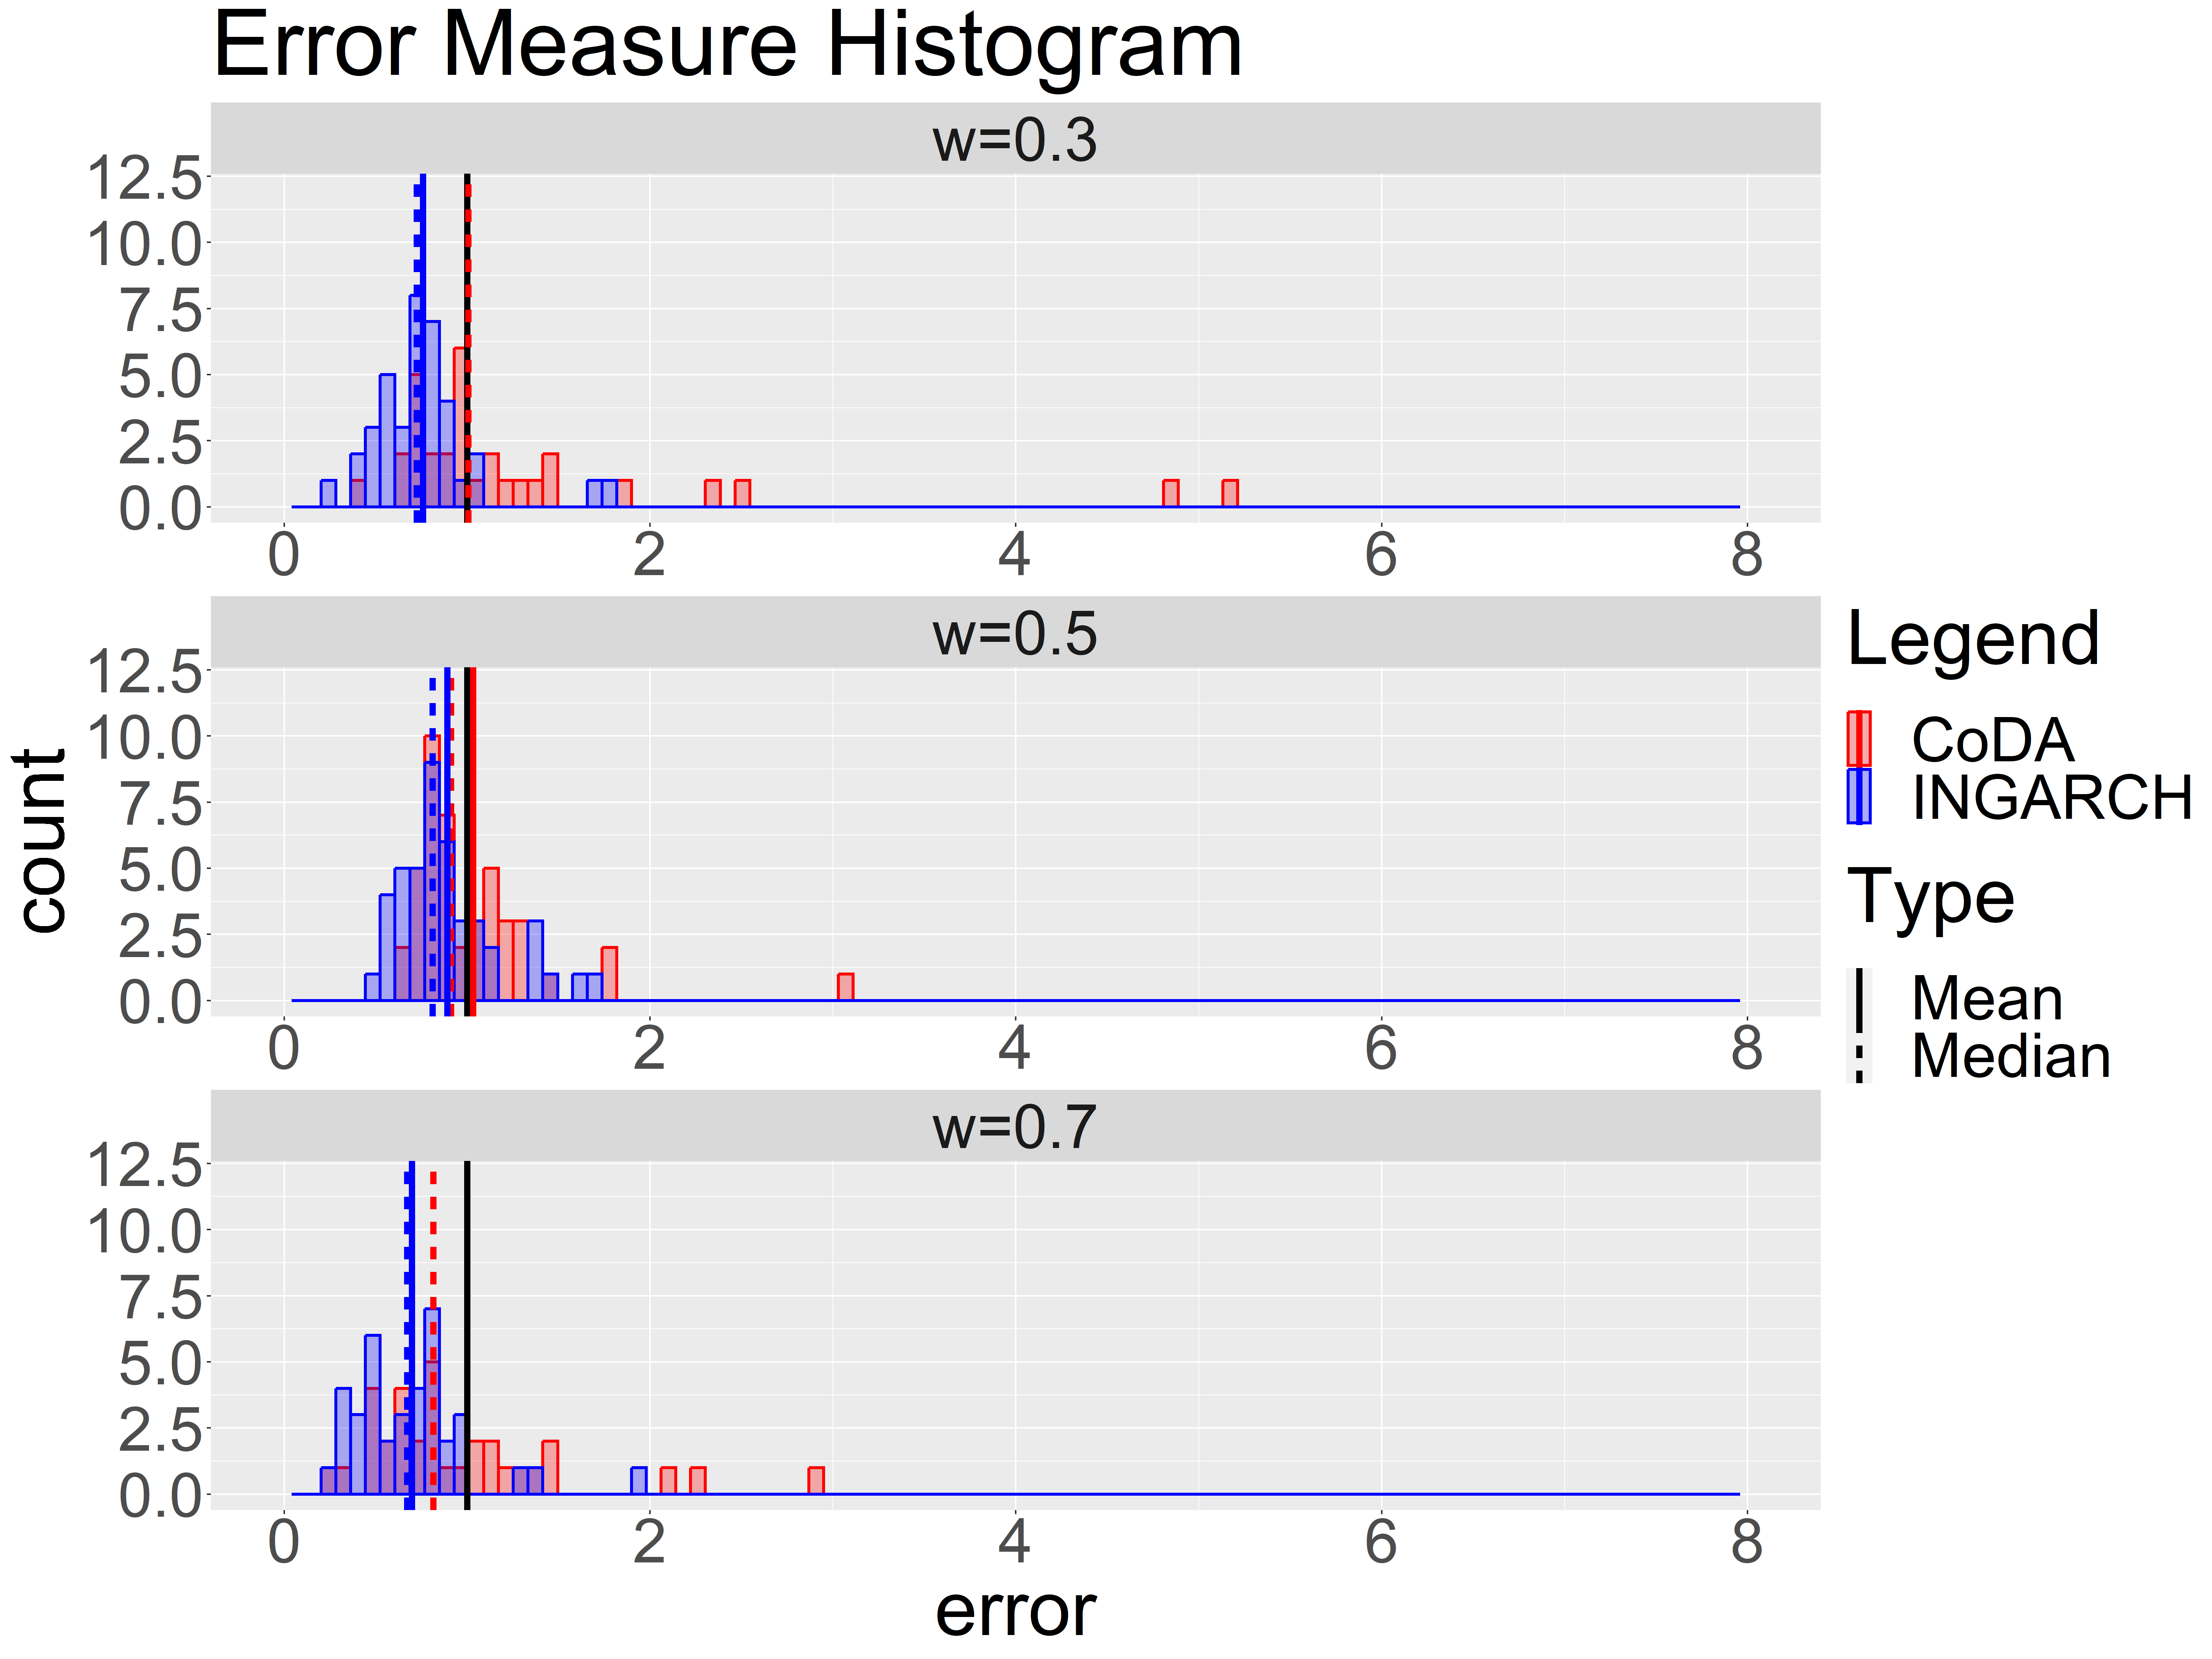
\includegraphics[width=\textwidth]{ErrorMeasureCombined_Histogram_all__Variation_frame.png}
\caption{Histogram of different $w$}
\label{fig:Frame Hist}
\end{subfigure}
\hfill
\begin{subfigure}[b]{0.8\textwidth}
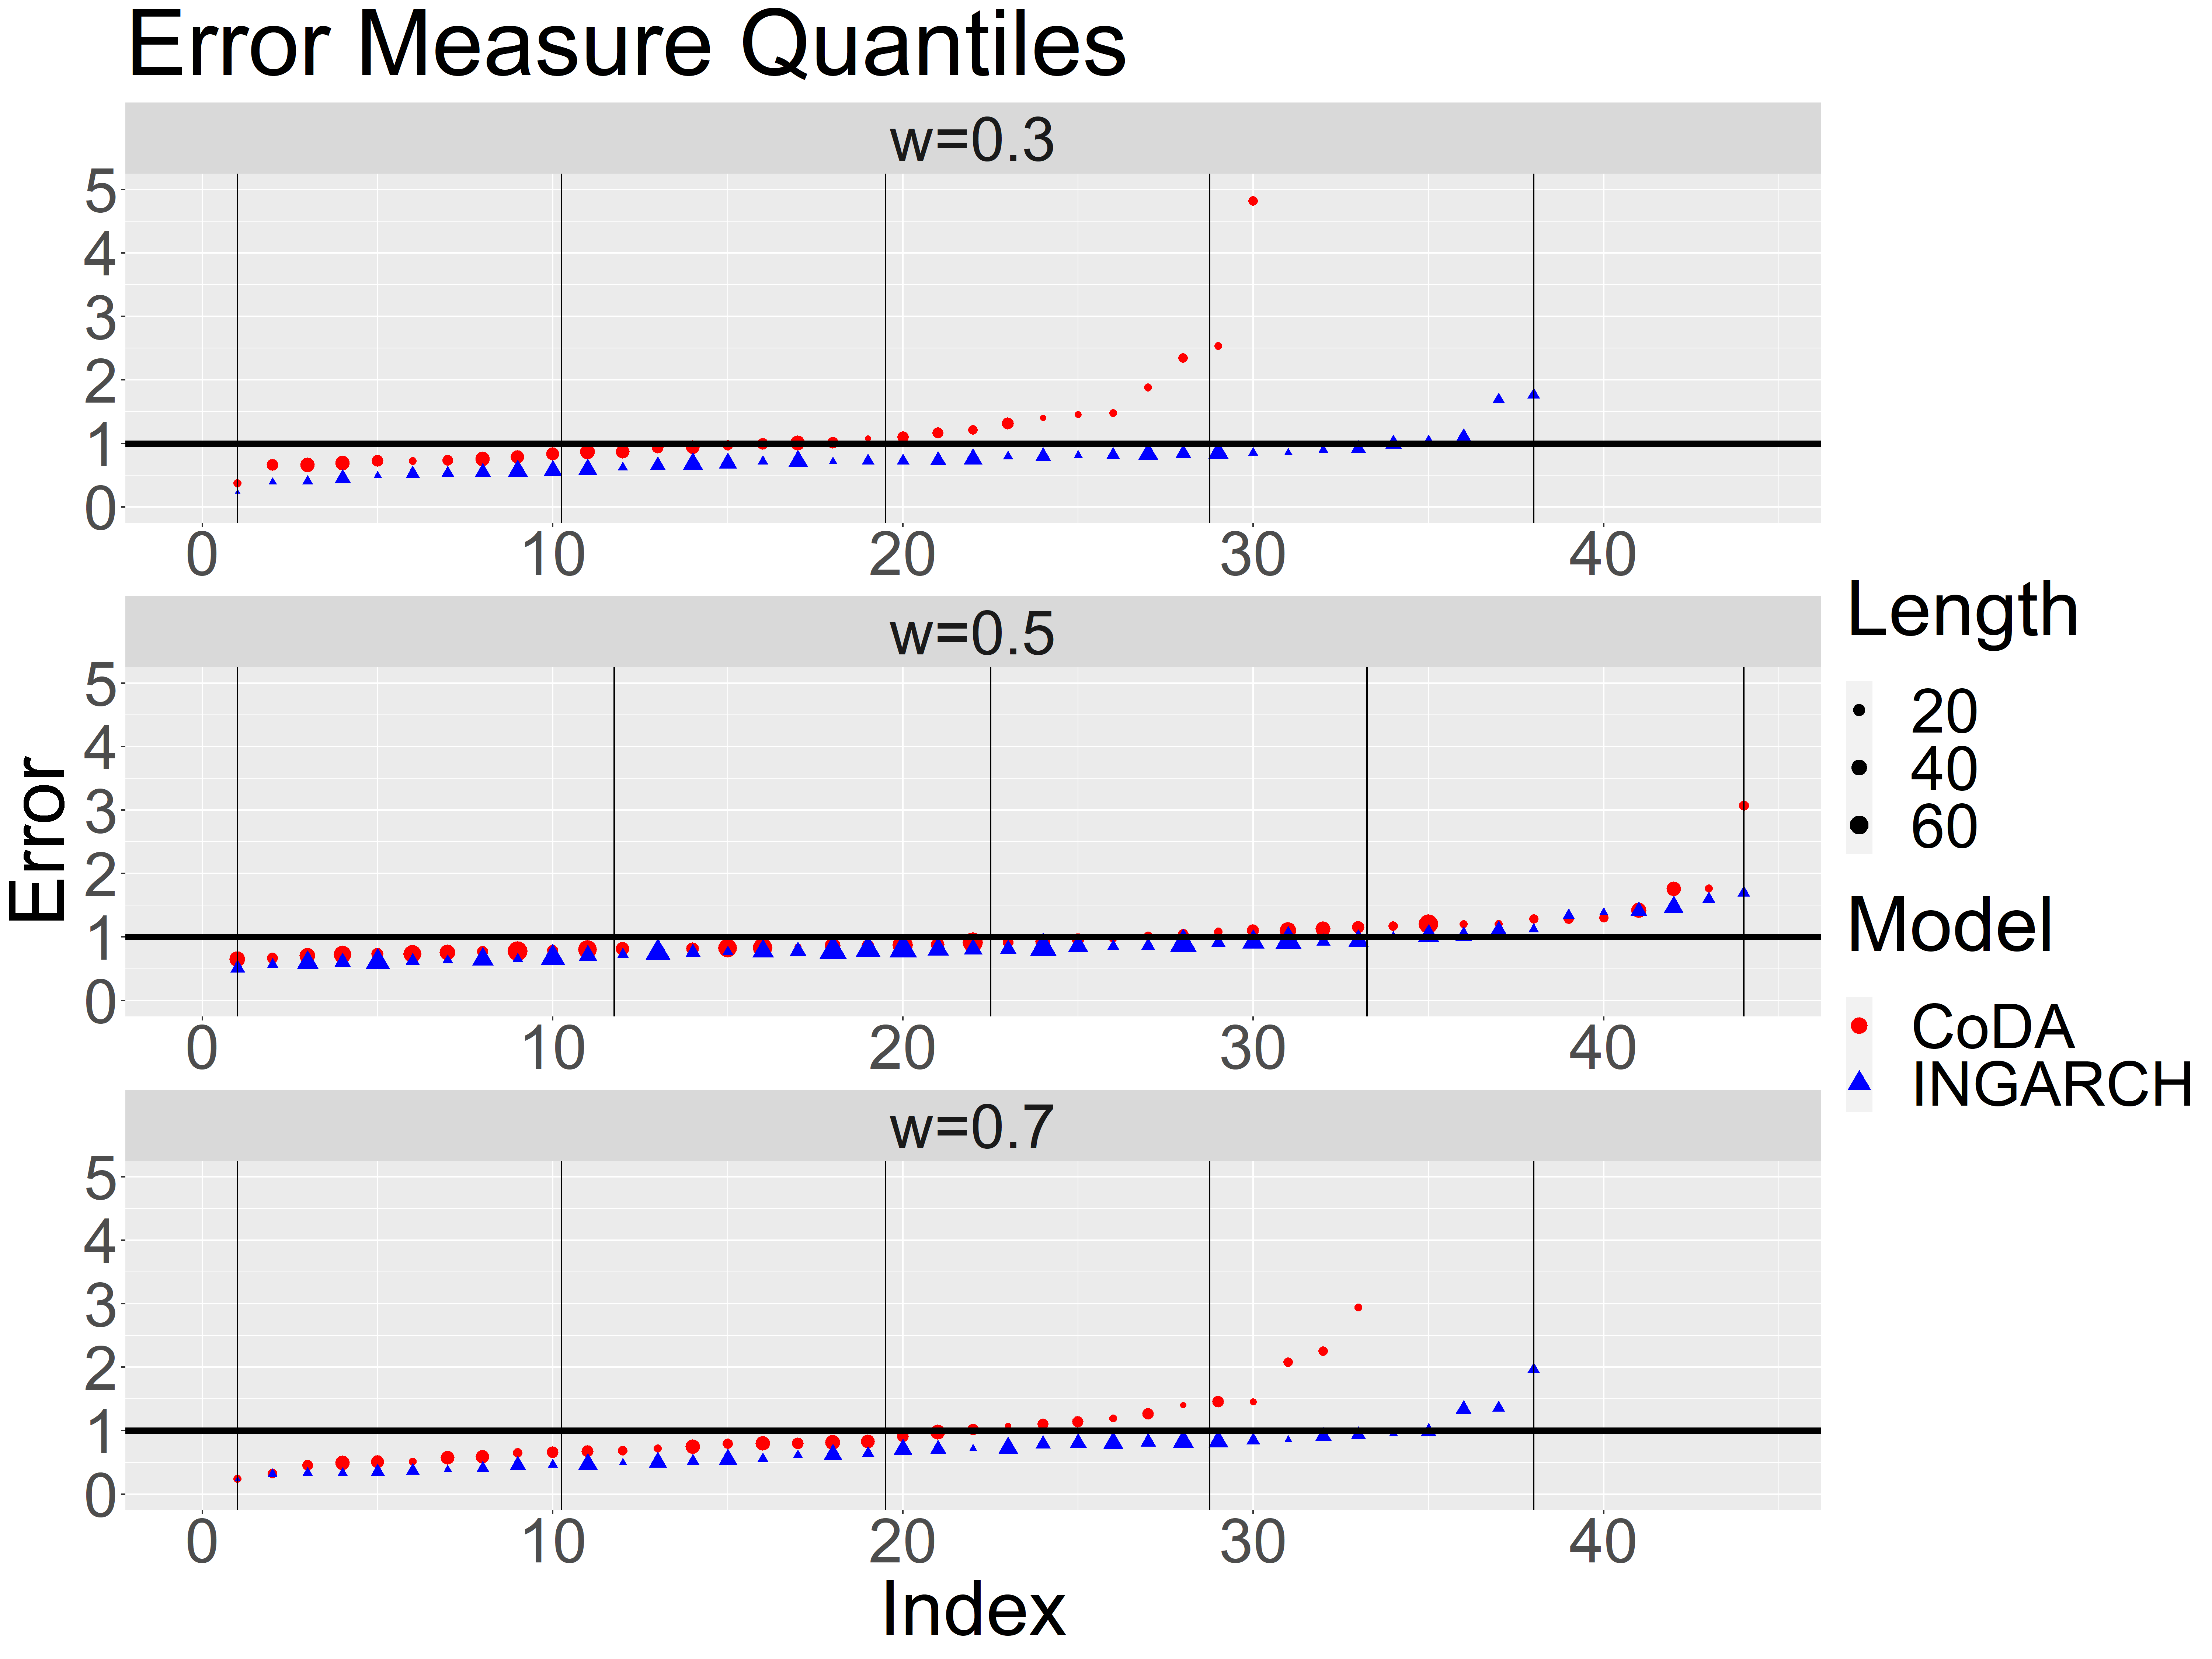
\includegraphics[width=\textwidth]{ErrorMeasureCombined_Quant_all__Variation_frame.png}
\caption{Quantiles of different $w$}
\label{fig:Frame Quant}
\end{subfigure}
\caption{Comparison of different $w$}
\label{fig:Frame Comp1}
\end{figure}


In the boxplot \ref{fig: Frame Box} it looks like INGARCH performs worst for $w=0.5$. However, in the quantile plot \ref{fig:Frame Quant} we can see that for $w=0.3,0.7$ the last errors are not included any more in the plot. This could either be a result of them being to high, or that the model couldn't be fit on those fridges. 

For CoDA there seems not to be much difference. The best results are obtained with $w=0.3$, but the differences are only marginal. 


\subsubsection{Window Shape}
\label{sec:Window Shape}

We also vary the shape of the window. As explained in \ref{sec: Model Specification} we either use a fixed amount of points and add and remove points as time goes on, or we continuously add points to the window. The results are in figures \ref{fig:window methods Comp1}. We can see that there are no big differences between the methods. For both, CoDA and INGARCH, there are no notable difference. 

\begin{figure}[htb!]
\centering
\begin{subfigure}[b]{0.45\textwidth}
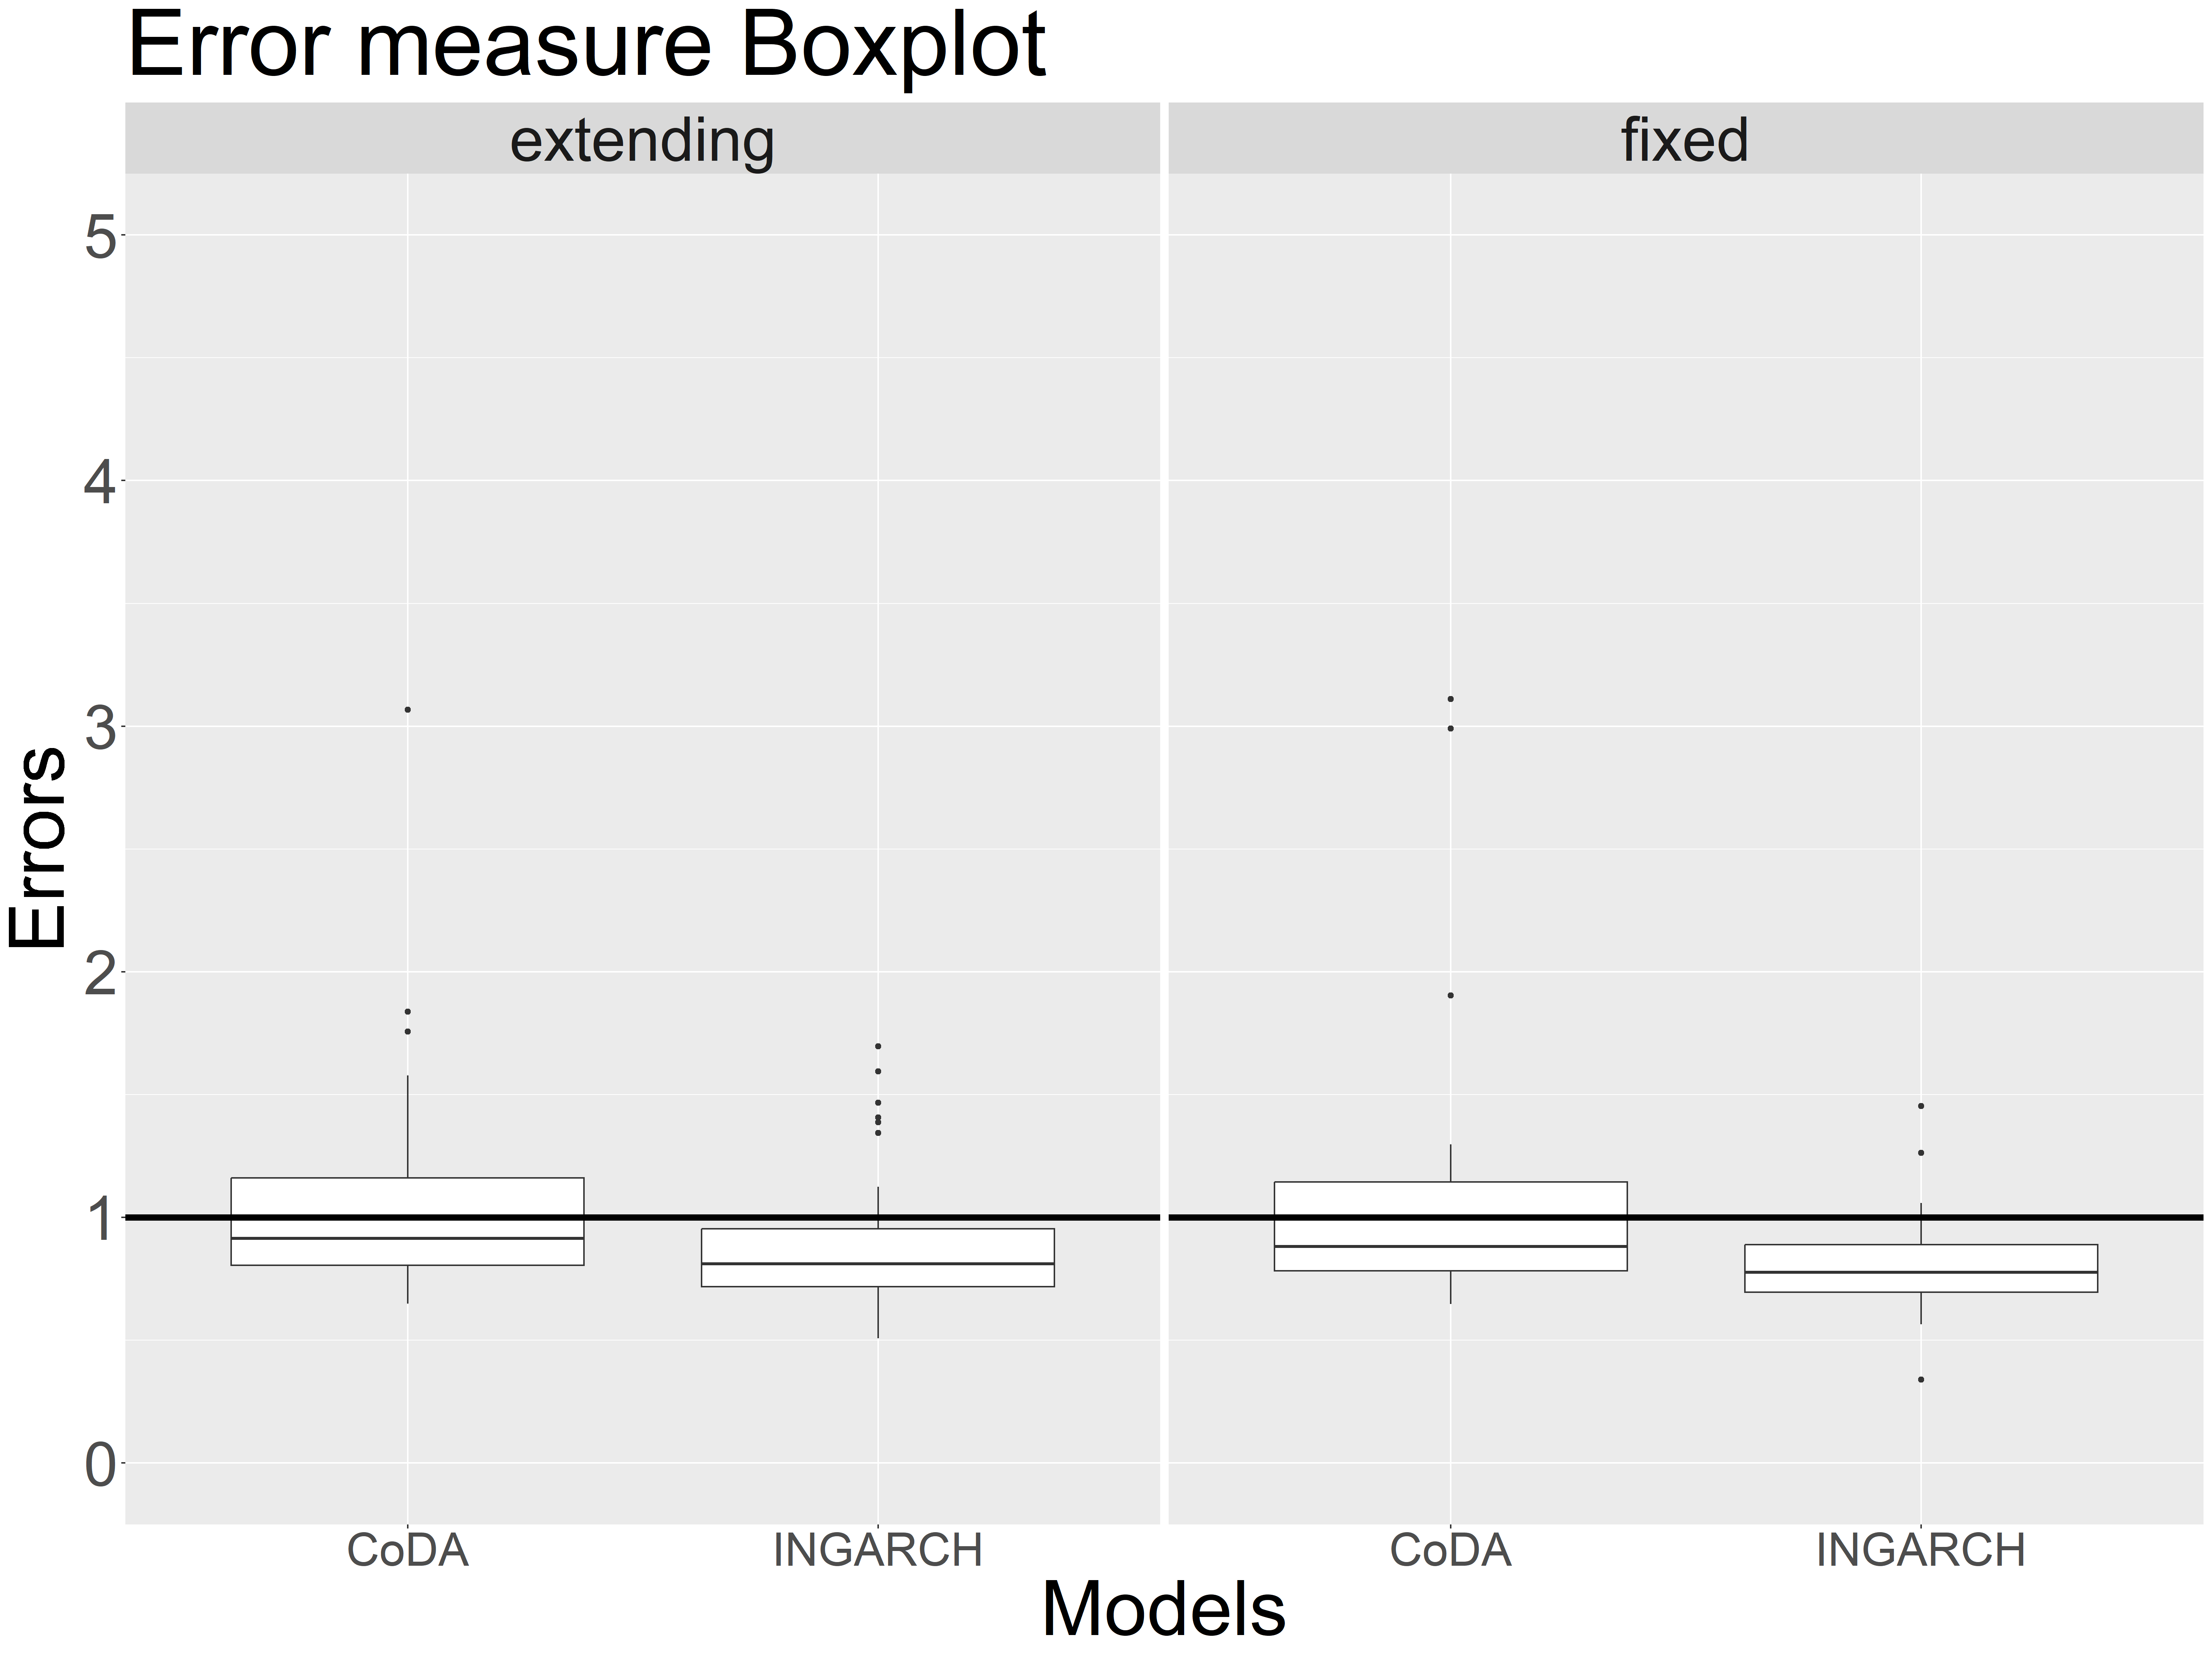
\includegraphics[width=\textwidth]{ErrorMeasureCombined_Box_all__Variation_windowMethod.png}
\caption{Boxplot for different window shapes}
\label{fig:window methods Box}
\end{subfigure}
\hfill
\begin{subfigure}[b]{0.45\textwidth}
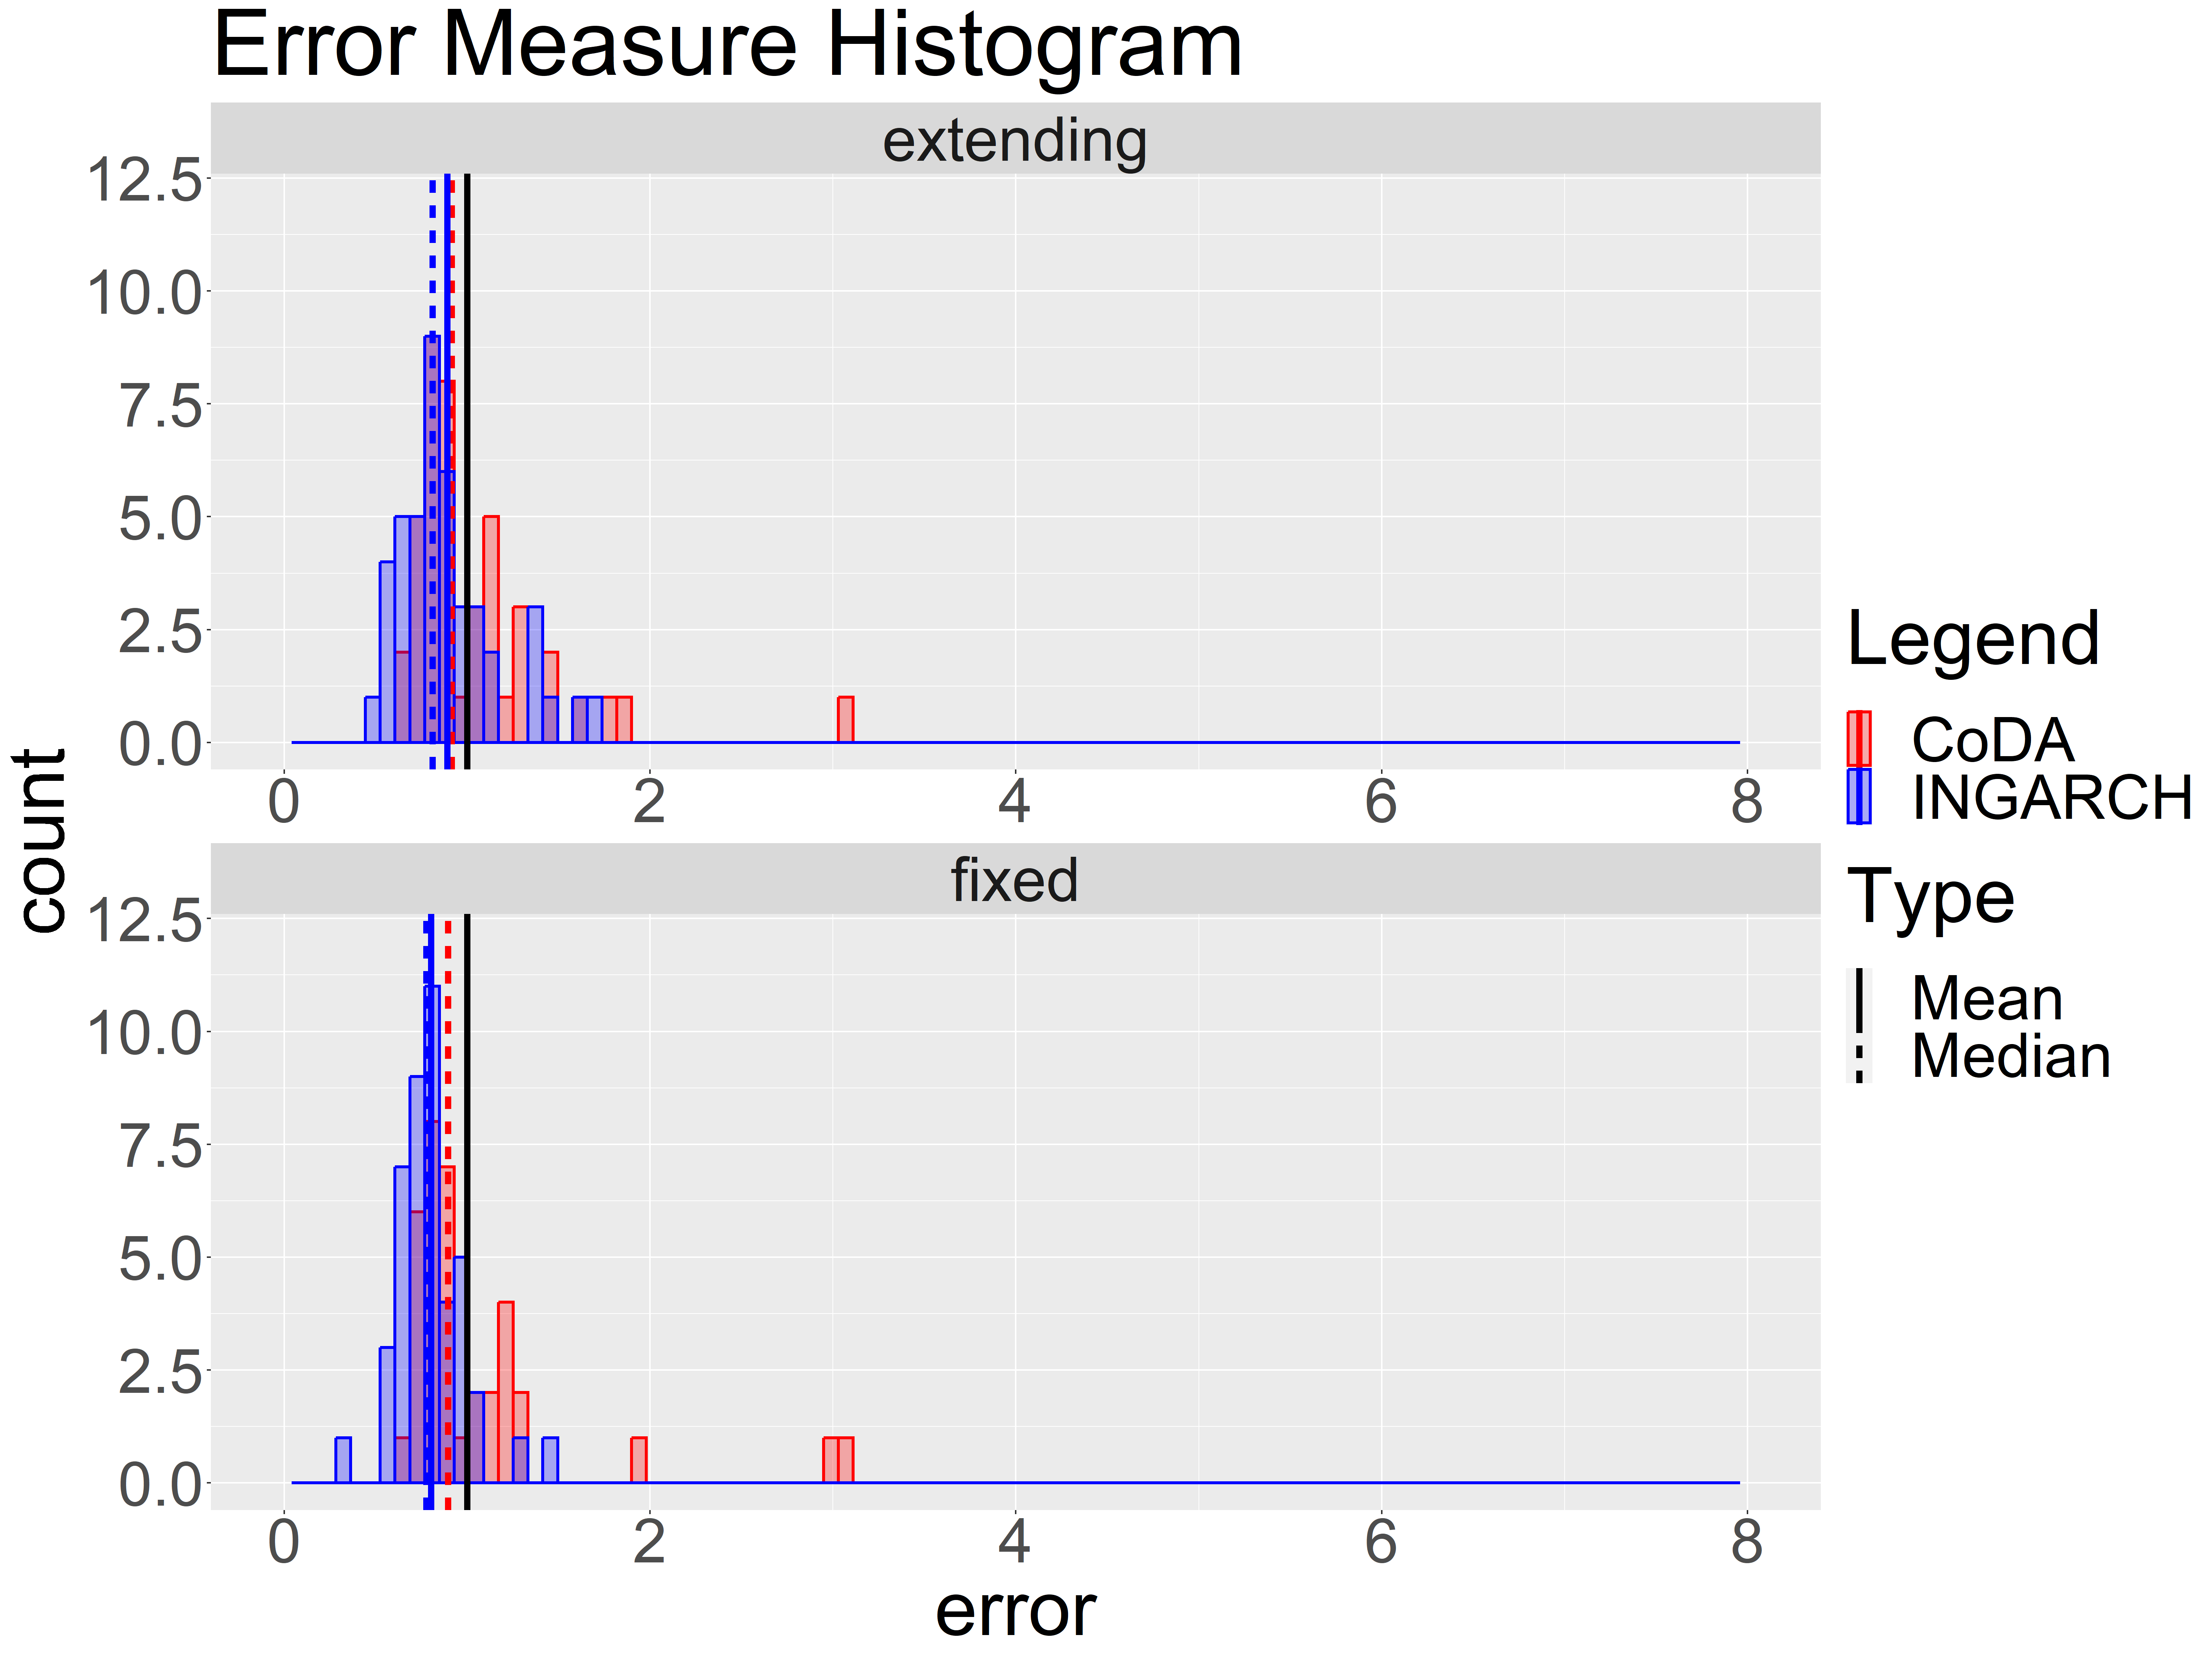
\includegraphics[width=\textwidth]{ErrorMeasureCombined_Histogram_all__Variation_windowMethod.png}
\caption{Histogram for different window shapes}
\label{fig:window methods Hist}
\end{subfigure}
\hfill
\begin{subfigure}[b]{0.8\textwidth}
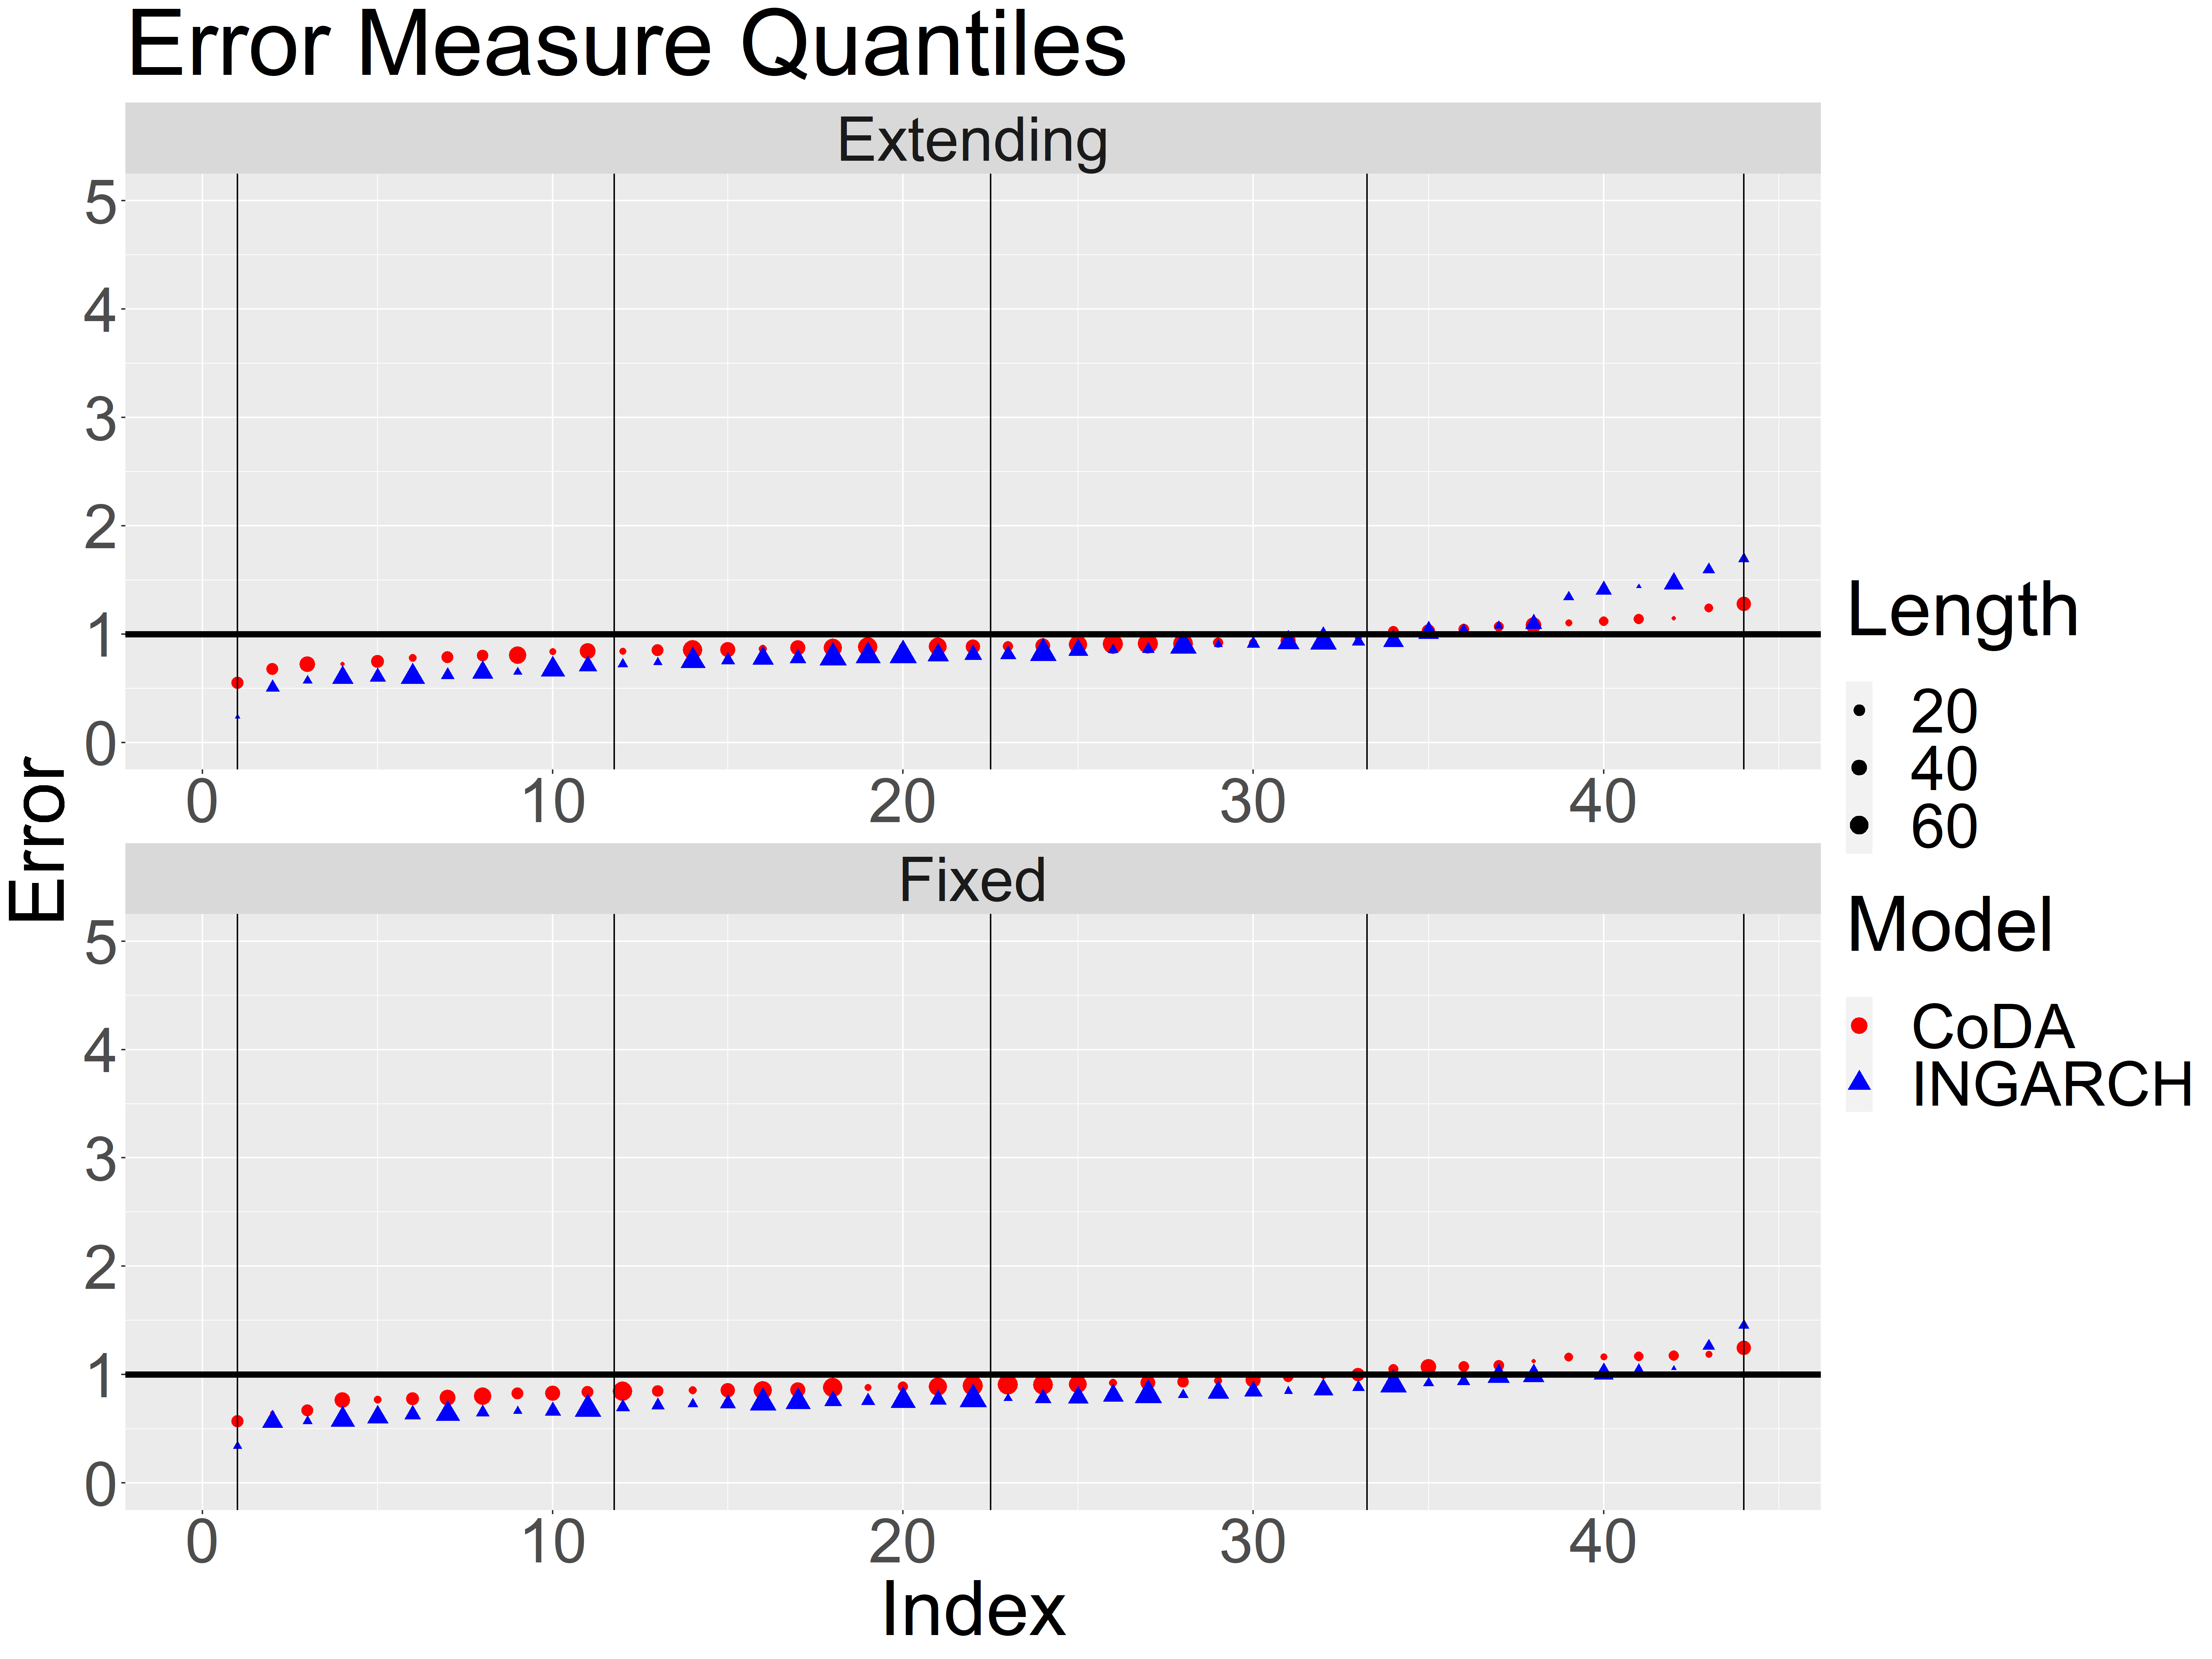
\includegraphics[width=\textwidth]{ErrorMeasureCombined_Quant_all__Variation_windowMethod.png}
\caption{Quantiles for different window shapes}
\label{fig:window methods Quant}
\end{subfigure}
\caption{Comparison of different window shapes}
\label{fig:window methods Comp1}
\end{figure}


\subsection{INGARCH Specifications Results}
\label{sec: Ingarch Specifications Results}

Next we will investigate the INGARCH specific options. As before we use the standard settings for the INGARCH(1,1) model and always vary one parameter. 

\subsubsection{Distribution}
\label{sec:Distribution}

As mentioned in \ref{sec: Ingarch Specifications} we can replace the Poisson distribution with a Negative Binomial Distribution in \ref{eq:Ingarch Distribution}. The results are shown in \ref{fig:distributions Comp1}. 

\begin{figure}[htb!]
\centering
\begin{subfigure}[b]{0.45\textwidth}
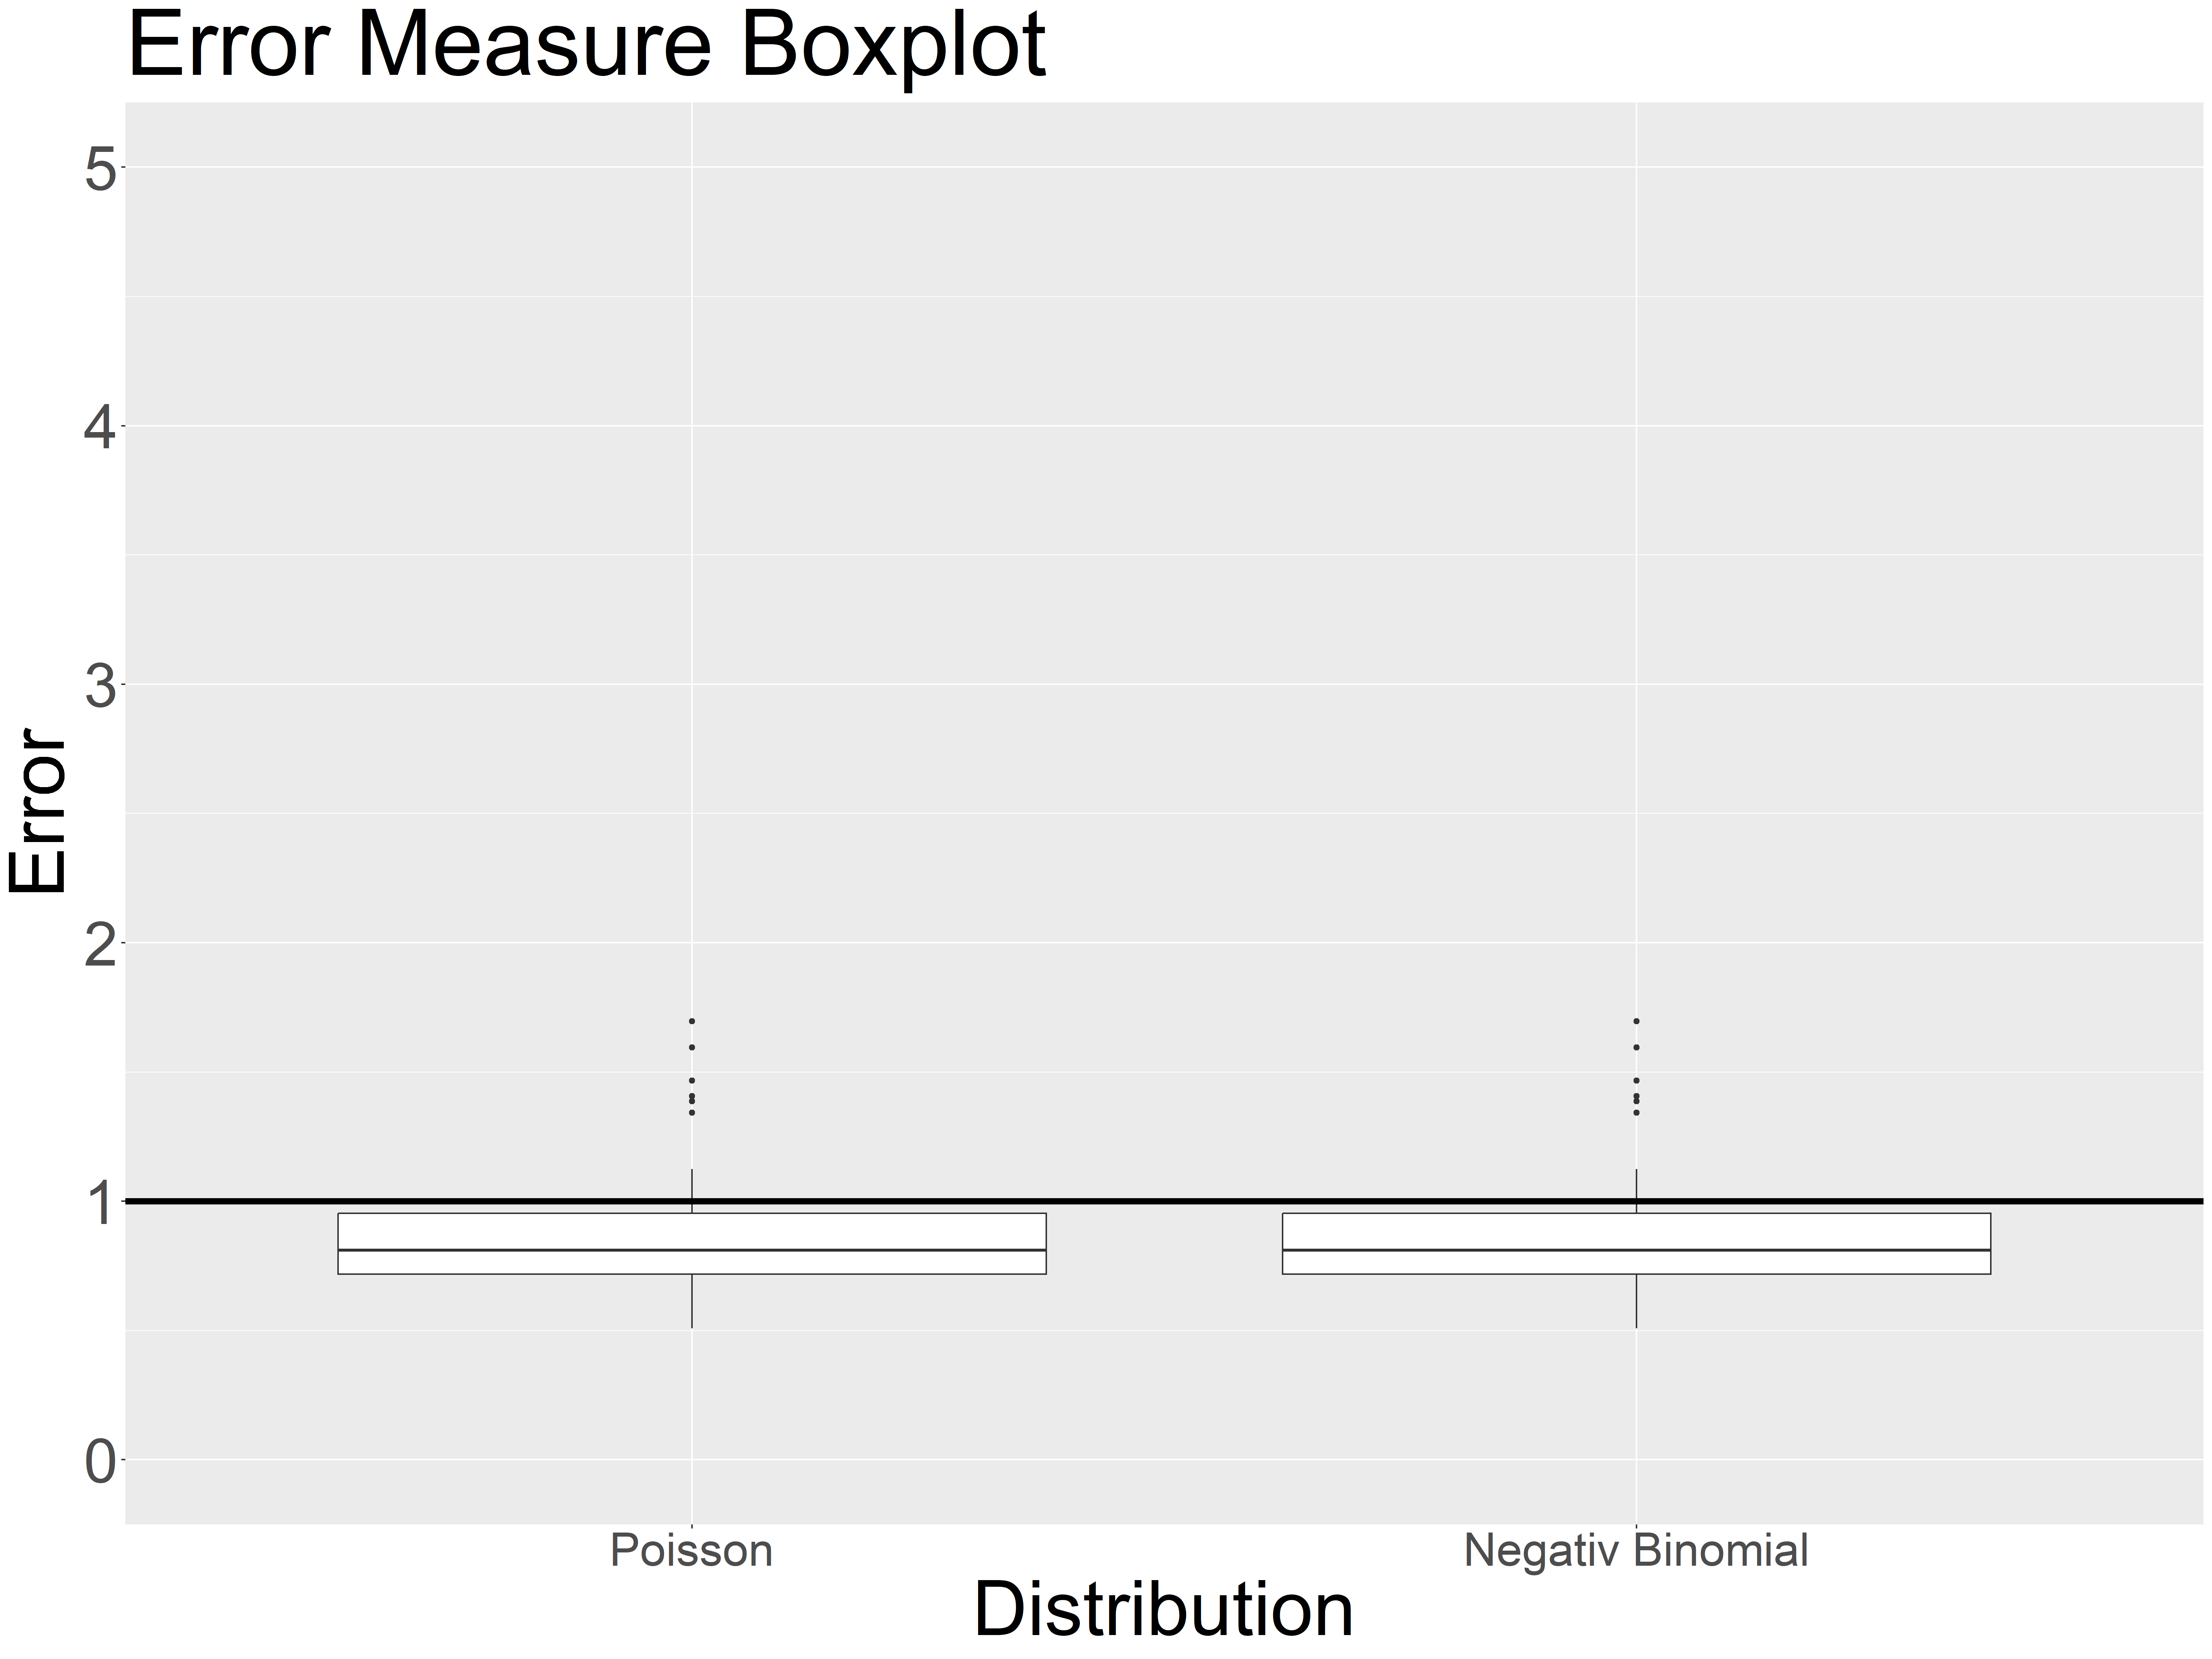
\includegraphics[width=\textwidth]{ErrorMeasureINGARCH_Box_all__Variation_distribution.png}
\caption{Boxplot for different distributions}
\label{fig:distributions Box}
\end{subfigure}
\hfill
\begin{subfigure}[b]{0.45\textwidth}
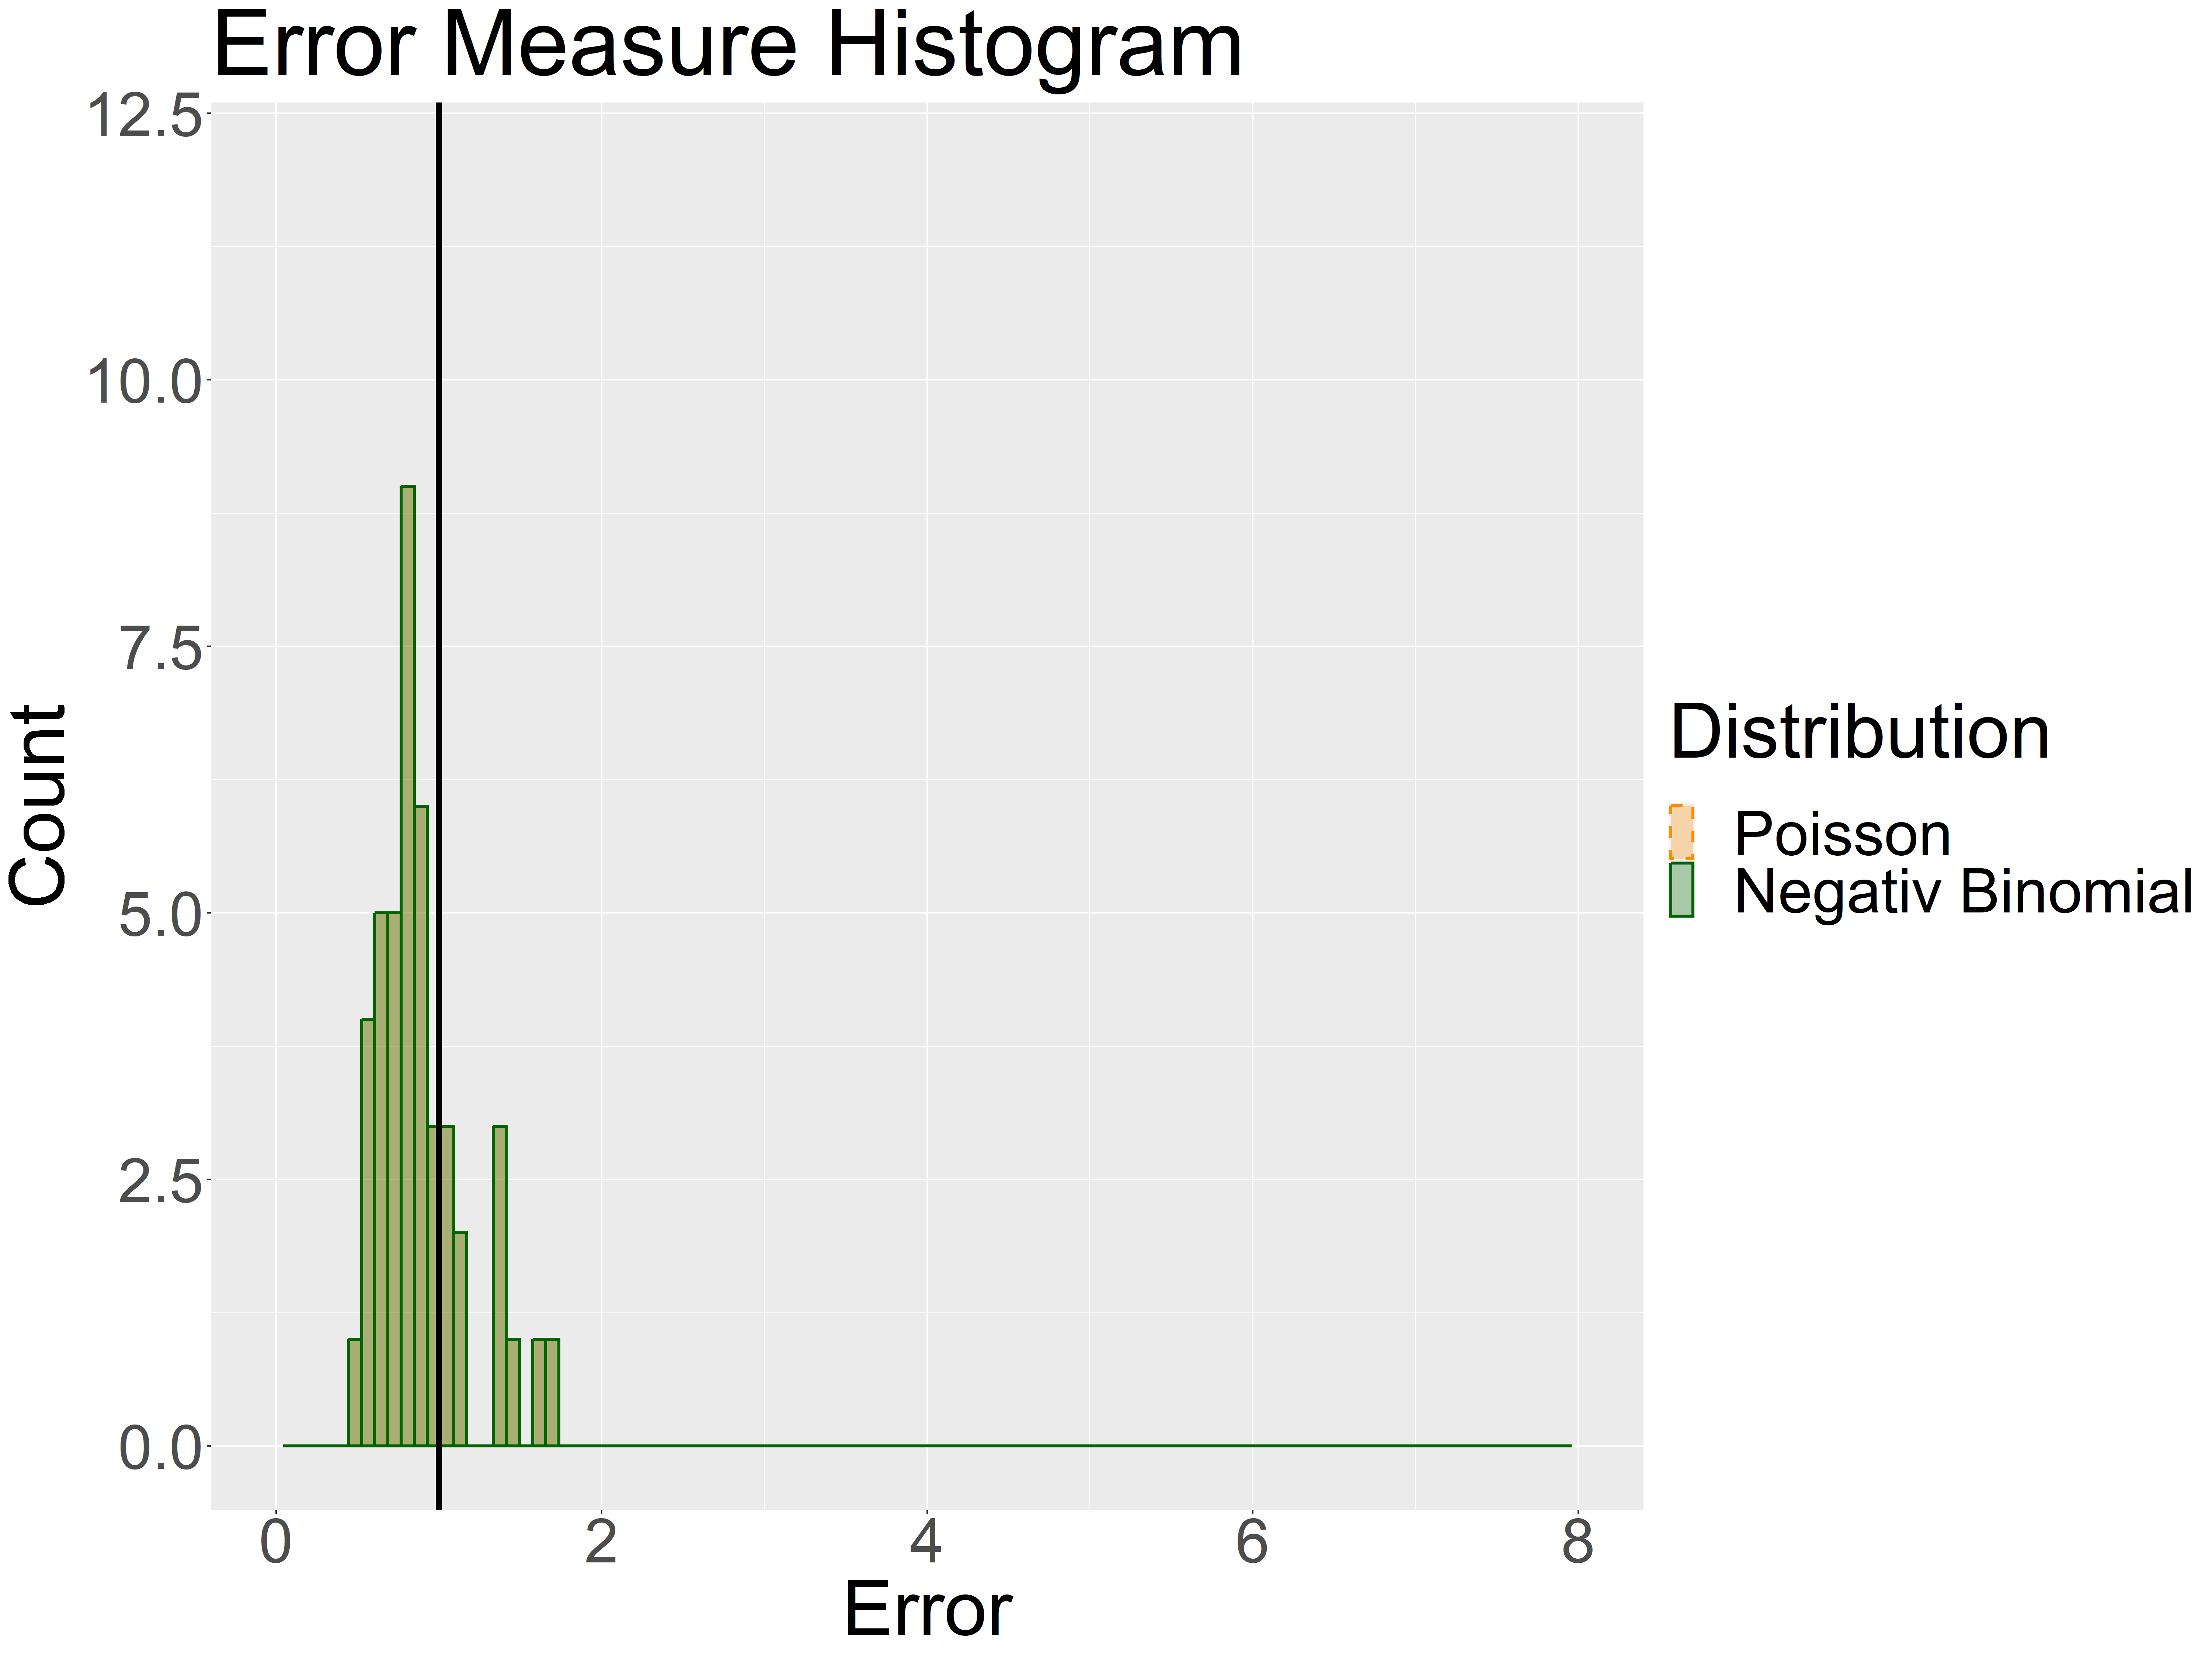
\includegraphics[width=\textwidth]{ErrorMeasureINGARCH_Histogram_all__Variation_distribution.png}
\caption{Histogram for different distributions}
\label{fig:distributions Hist}
\end{subfigure}
\hfill
%\begin{subfigure}[b]{0.8\textwidth}
%\includegraphics[width=\textwidth]{ErrorMeasureINGARCH_Quant_all__Variation_windowMethod.png}
%\caption{Quantiles for different distributions}
%\label{fig:window methods Quant}
%\end{subfigure}
\caption{Comparison of different distributions}
\label{fig:distributions Comp1}
\end{figure}

As we can see, we get the exactly the same results for both distributions. However, as mentioned in \ref{sec: Estimation of the Ingarch Model}, we round the predicted conditional mean to the next integer. Hence we could get slightly different results for the different distributions. Nevertheless, the difference is still negligible. %Since the Poisson Distribution is a limiting case of the Negative Binomial Distribution when $\phi \longrightarrow \infty$ in \ref{eq:Ingarch negbinom Distribution}, \cite{Liboschik:2016}. 


\subsubsection{Number of Past Means and Observations}
\label{sec: Number of Past Means and Observations}

The order in the INGARCH(p,q) model is another parameter which can be chosen. For simplicities sake we only compare our INGARCH(1,1) with an INGARCH(1,2) and INGARCH(2,1) model. However, further models could be tried out and compared. One could even optimise over the optimal order. 

In figure \ref{fig:past means Comp1} we compare the INGARCH(1,1) model (red) with the INGARCH(1,2) model (blue). We can see that the performance is very similar. Hence we prefer the smaller model. 
\begin{figure}[htb!]
\centering
\begin{subfigure}[b]{0.45\textwidth}
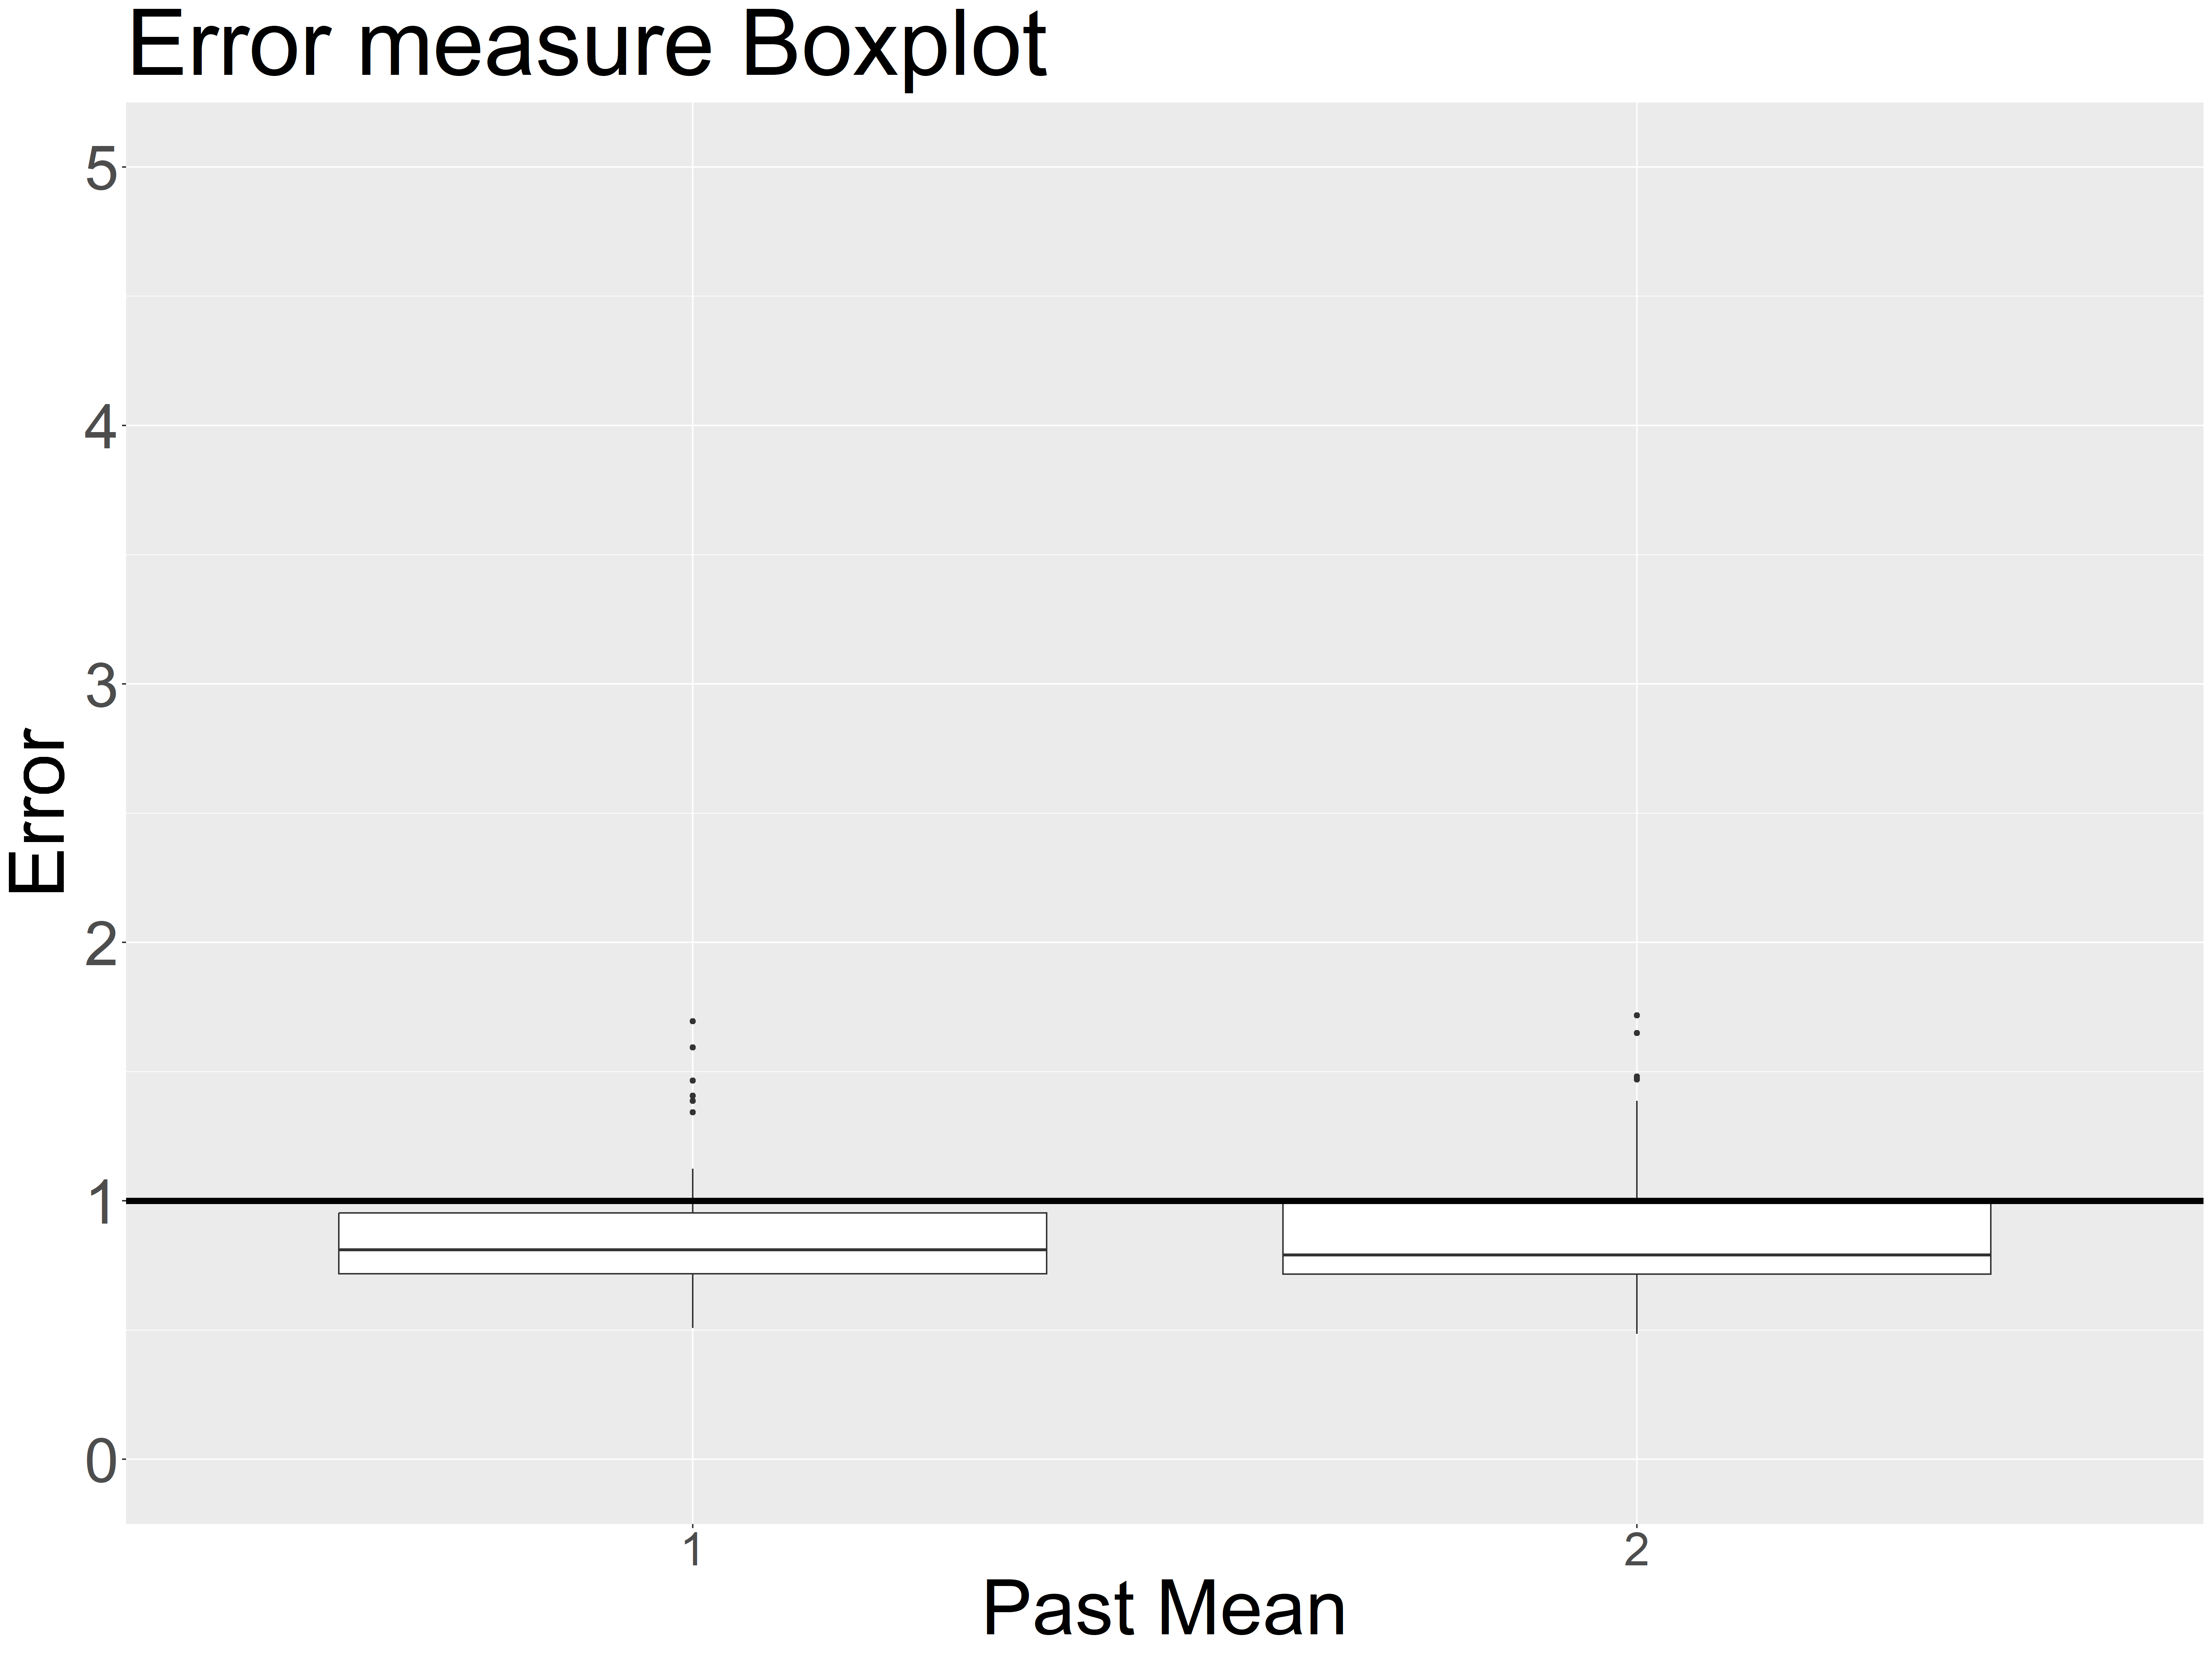
\includegraphics[width=\textwidth]{ErrorMeasureINGARCH_Box_all__Variation_pastMean.png}
\caption{Boxplot for a different number of past means}
\label{fig:past means Box}
\end{subfigure}
\hfill
\begin{subfigure}[b]{0.45\textwidth}
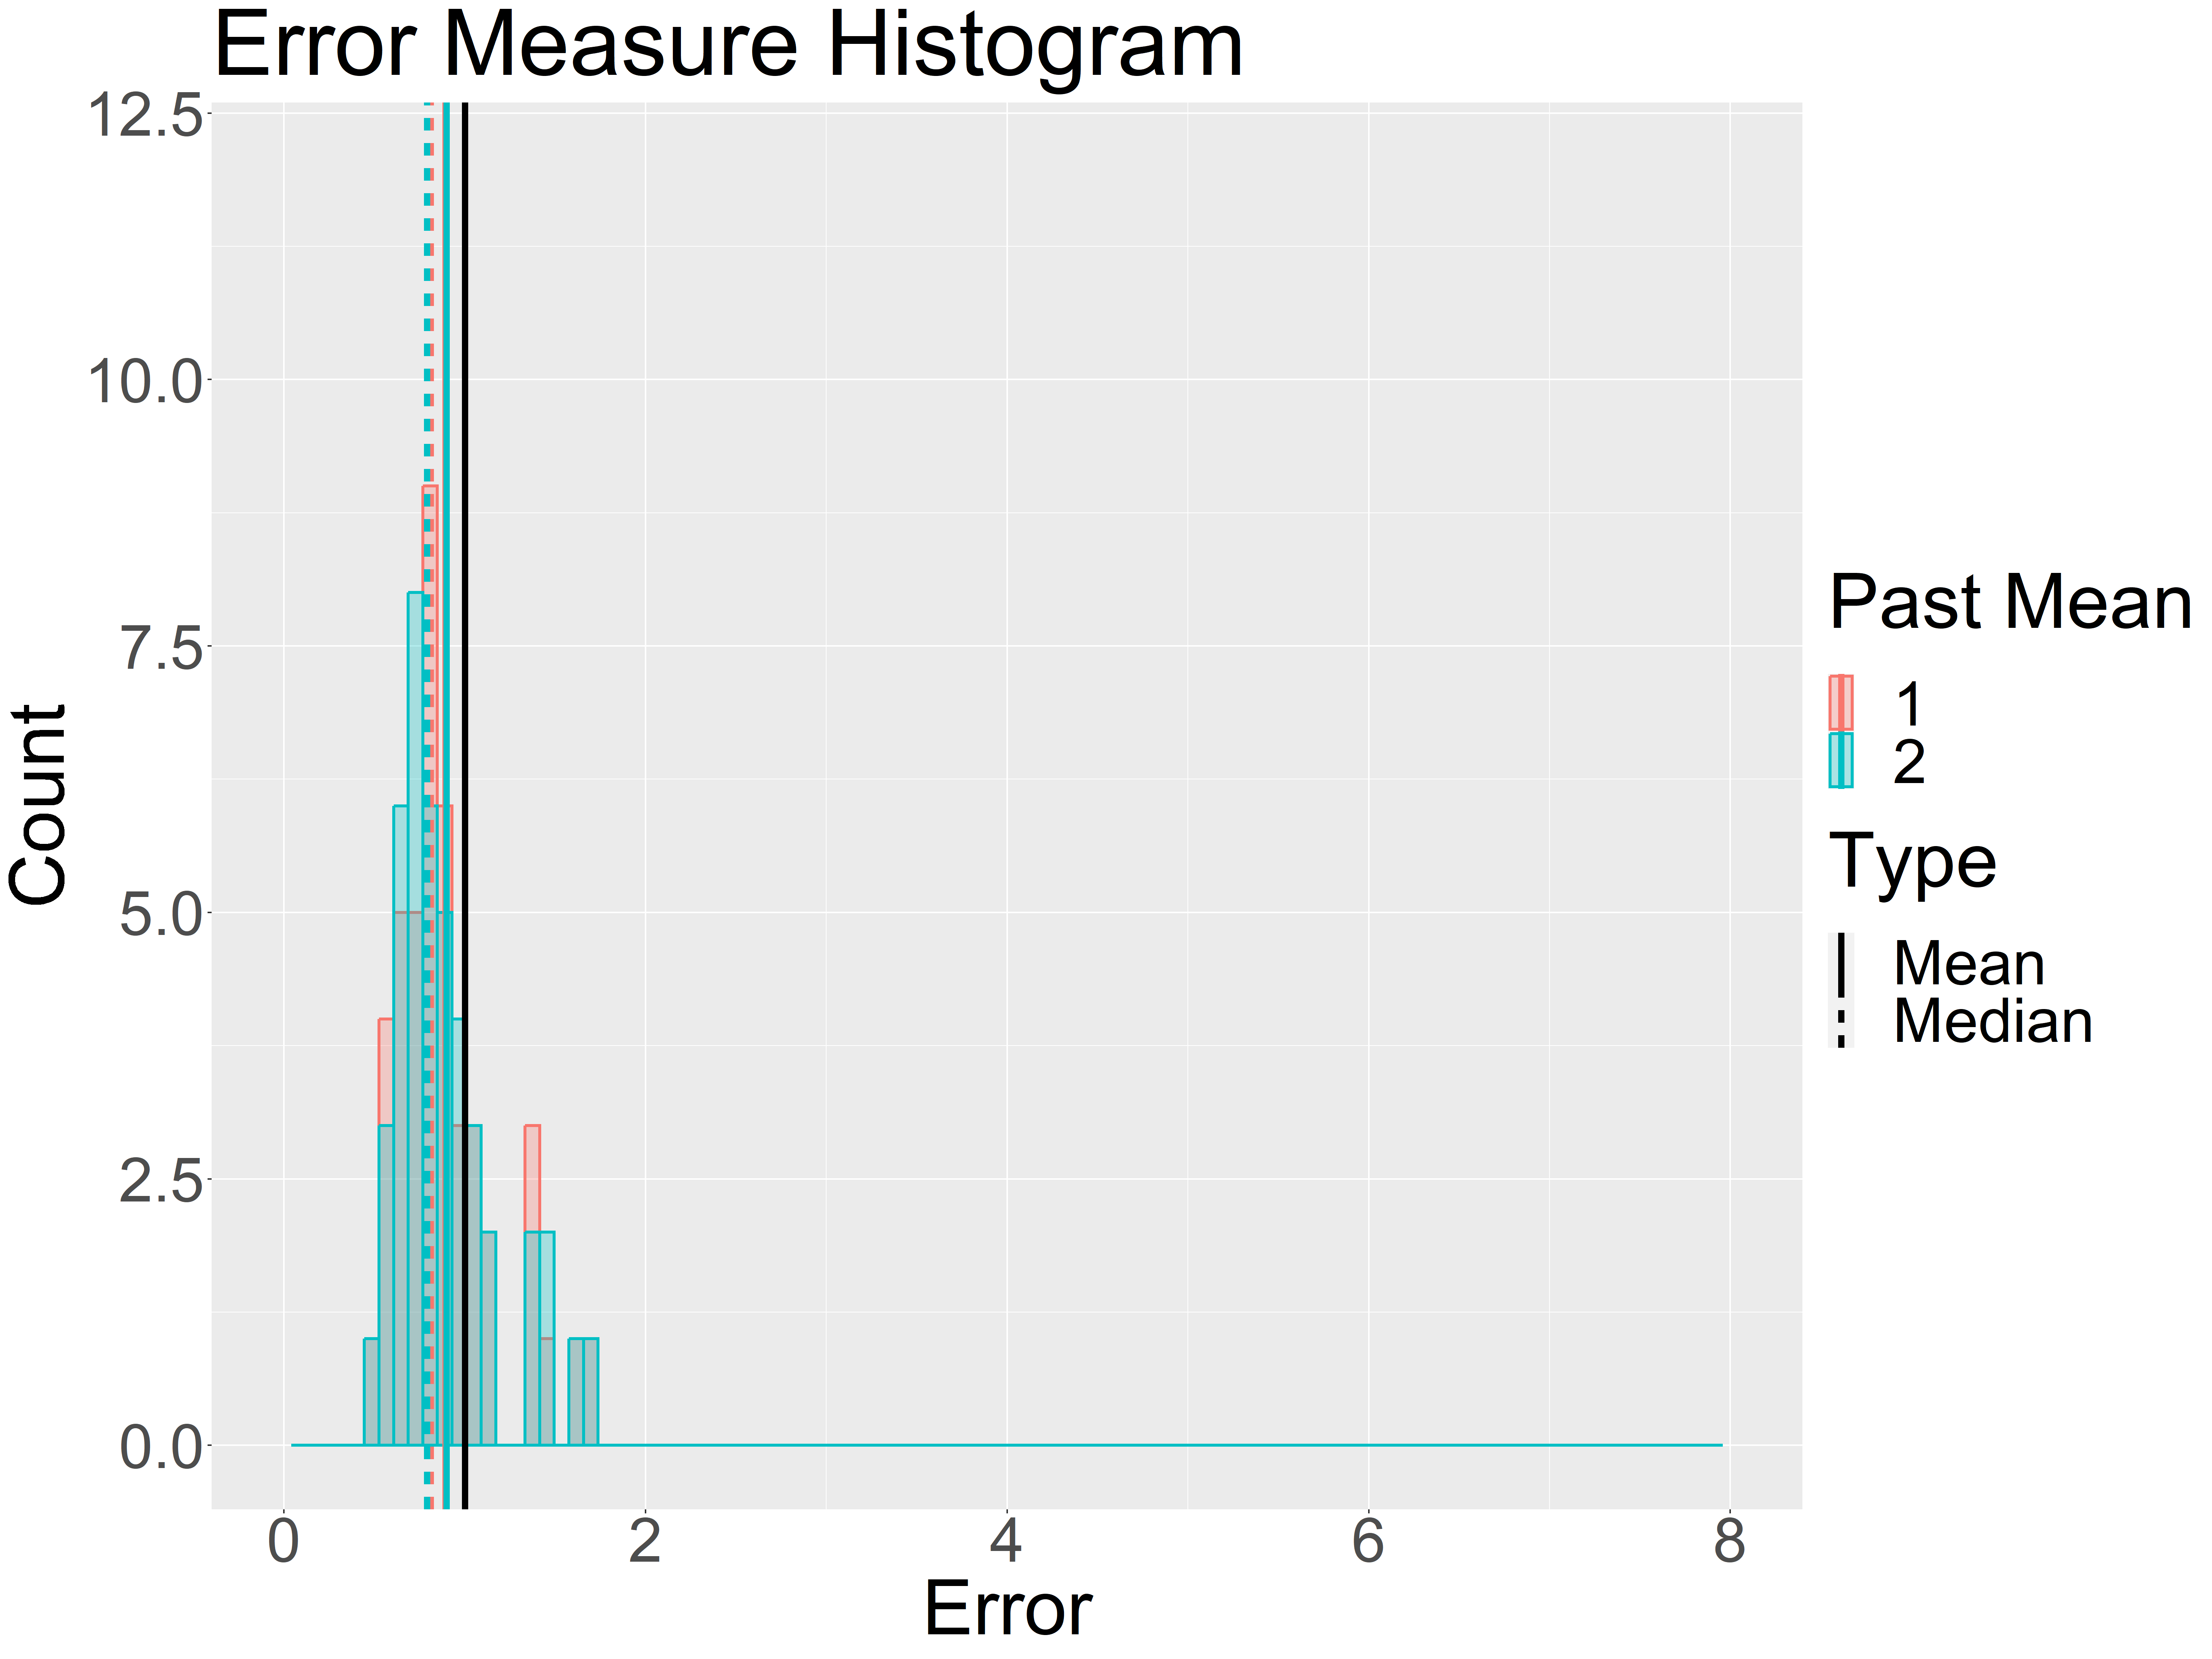
\includegraphics[width=\textwidth]{ErrorMeasureINGARCH_Histogram_all__Variation_pastMean.png}
\caption{Histogram for a different number of past means}
\label{fig:past means Hist}
\end{subfigure}
\hfill
\begin{subfigure}[b]{0.8\textwidth}
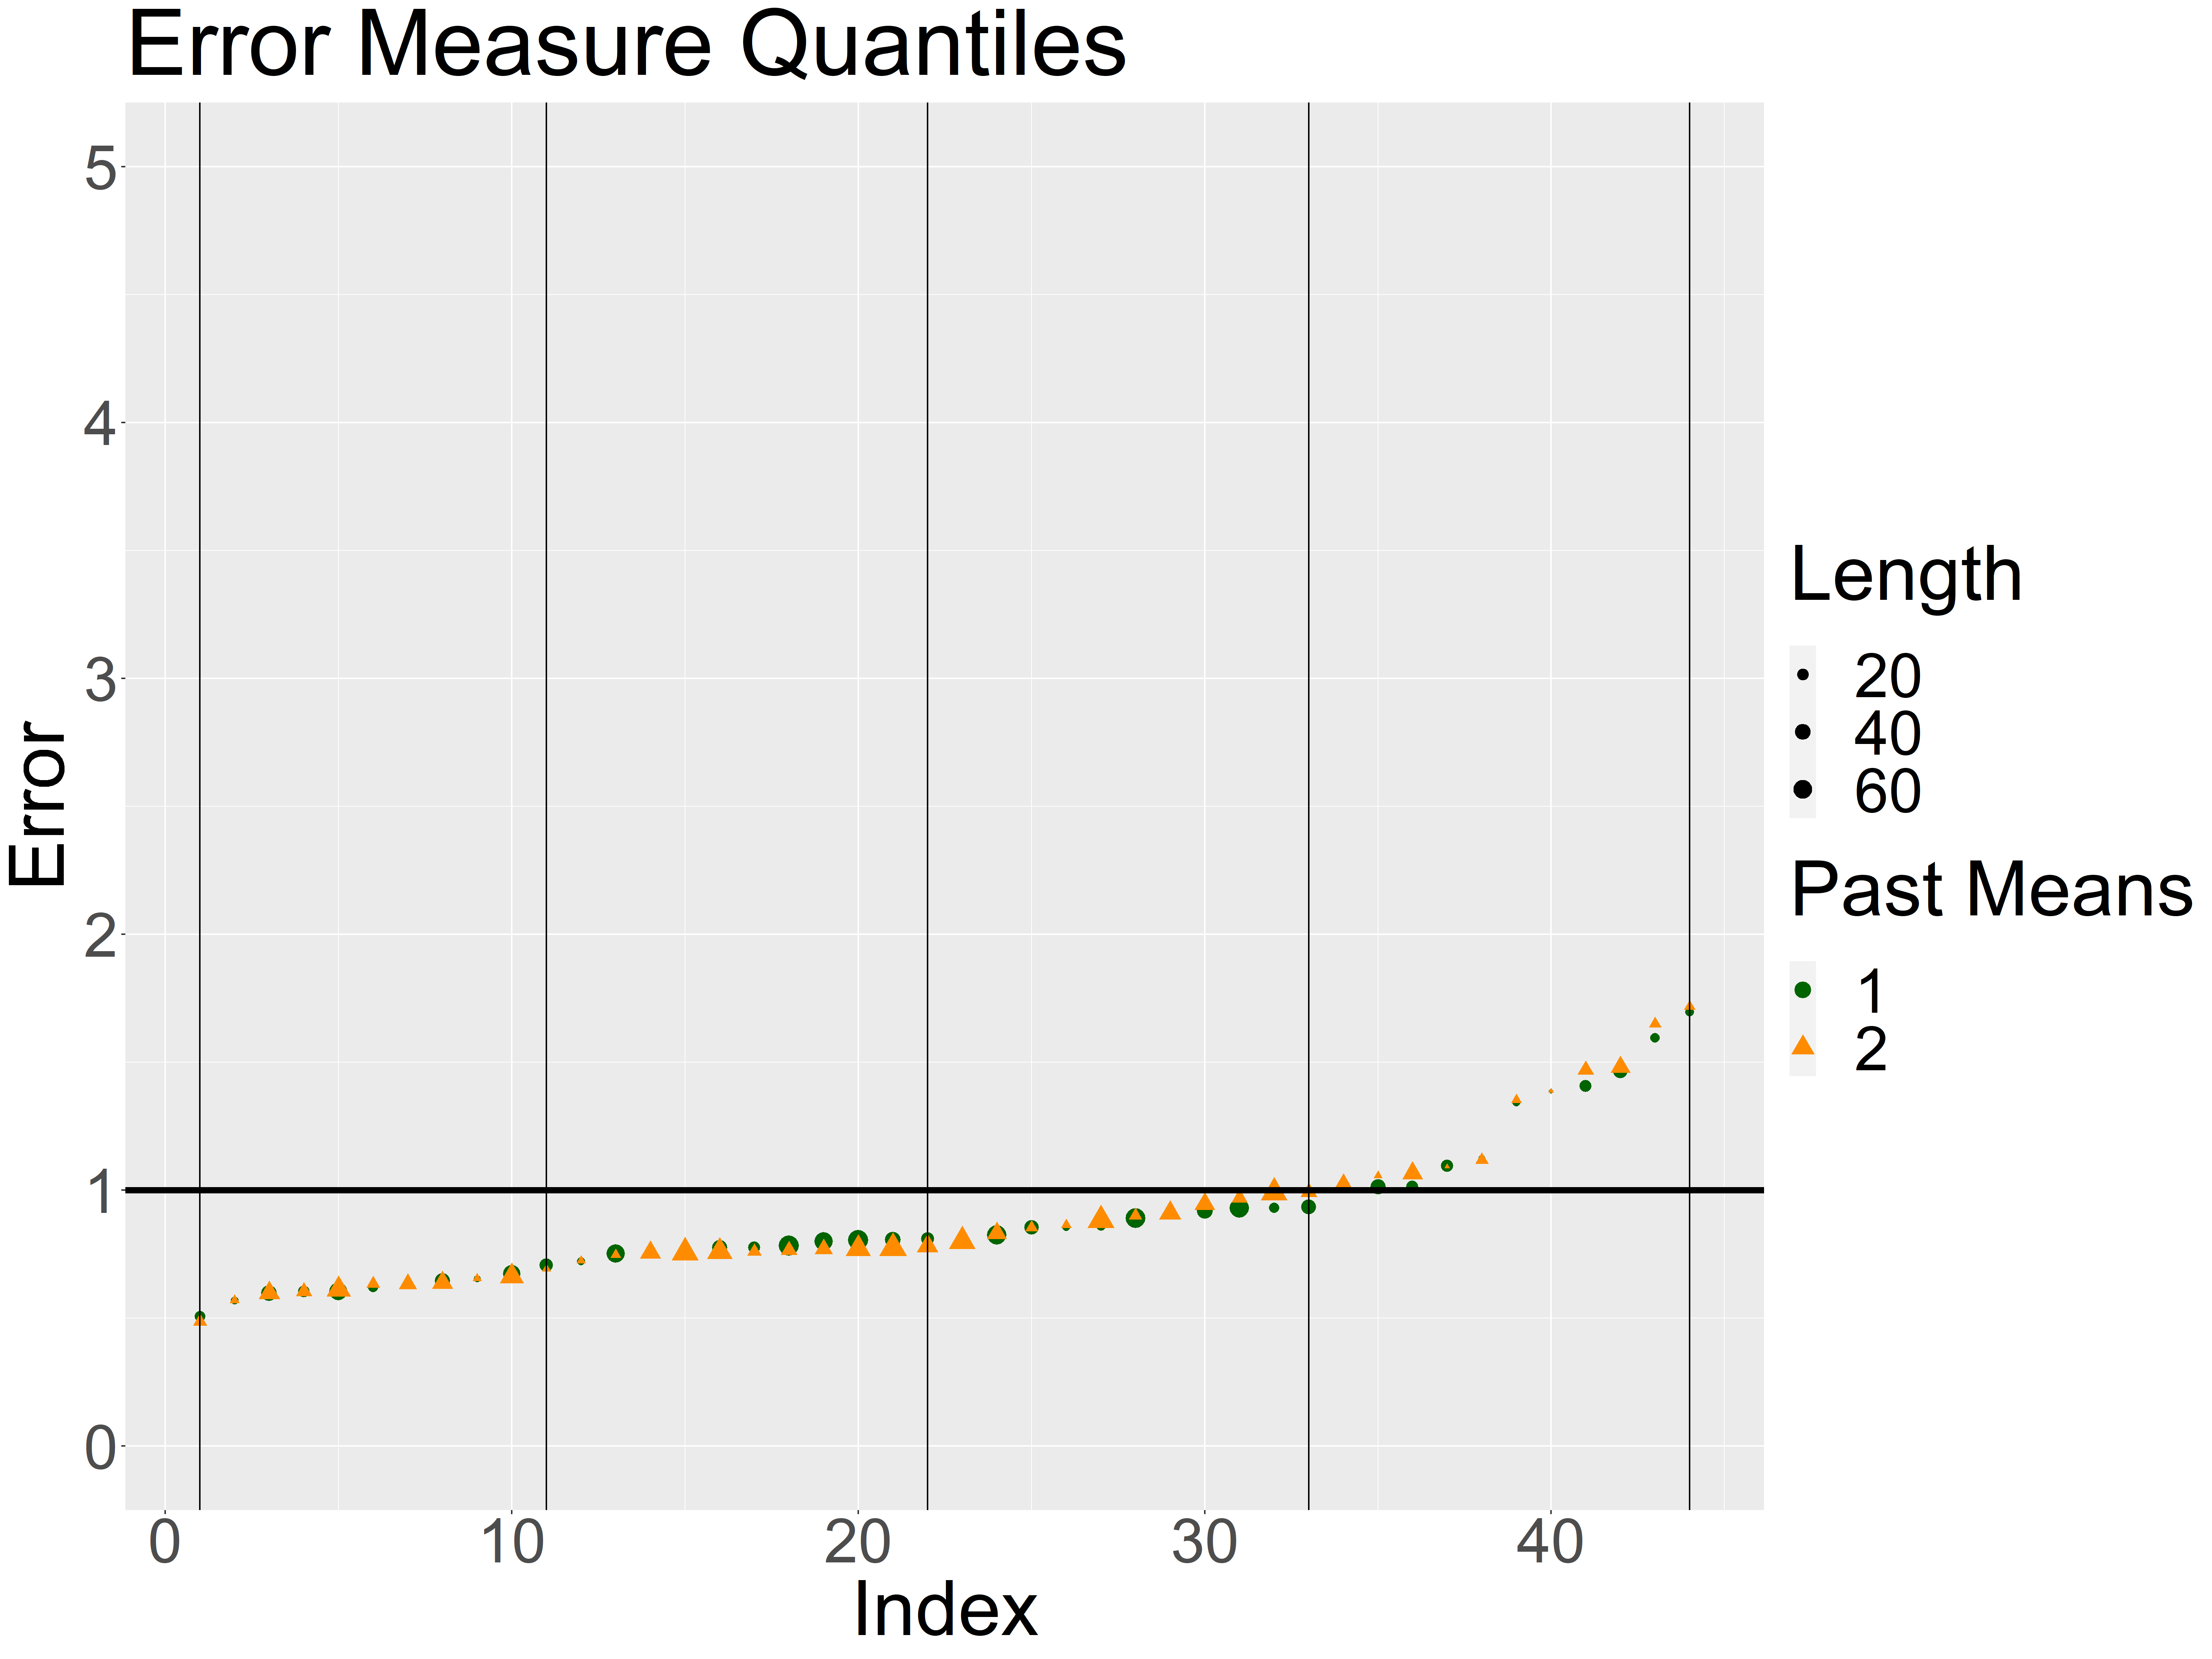
\includegraphics[width=\textwidth]{ErrorMeasureINGARCH_Quant_all__Variation_pastMean.png}
\caption{Quantiles for a different number of past means}
\label{fig:past means Quant}
\end{subfigure}
\caption{Comparison of a different number of past means}
\label{fig:past means Comp1}
\end{figure}


In figure \ref{fig:past obs Comp1} we compare the INGARCH(1,1) (red) model with the INGARCH(2,1) (blue) model. Again the performance is very similar in general. 

\begin{figure}[htb!]
\centering
\begin{subfigure}[b]{0.45\textwidth}
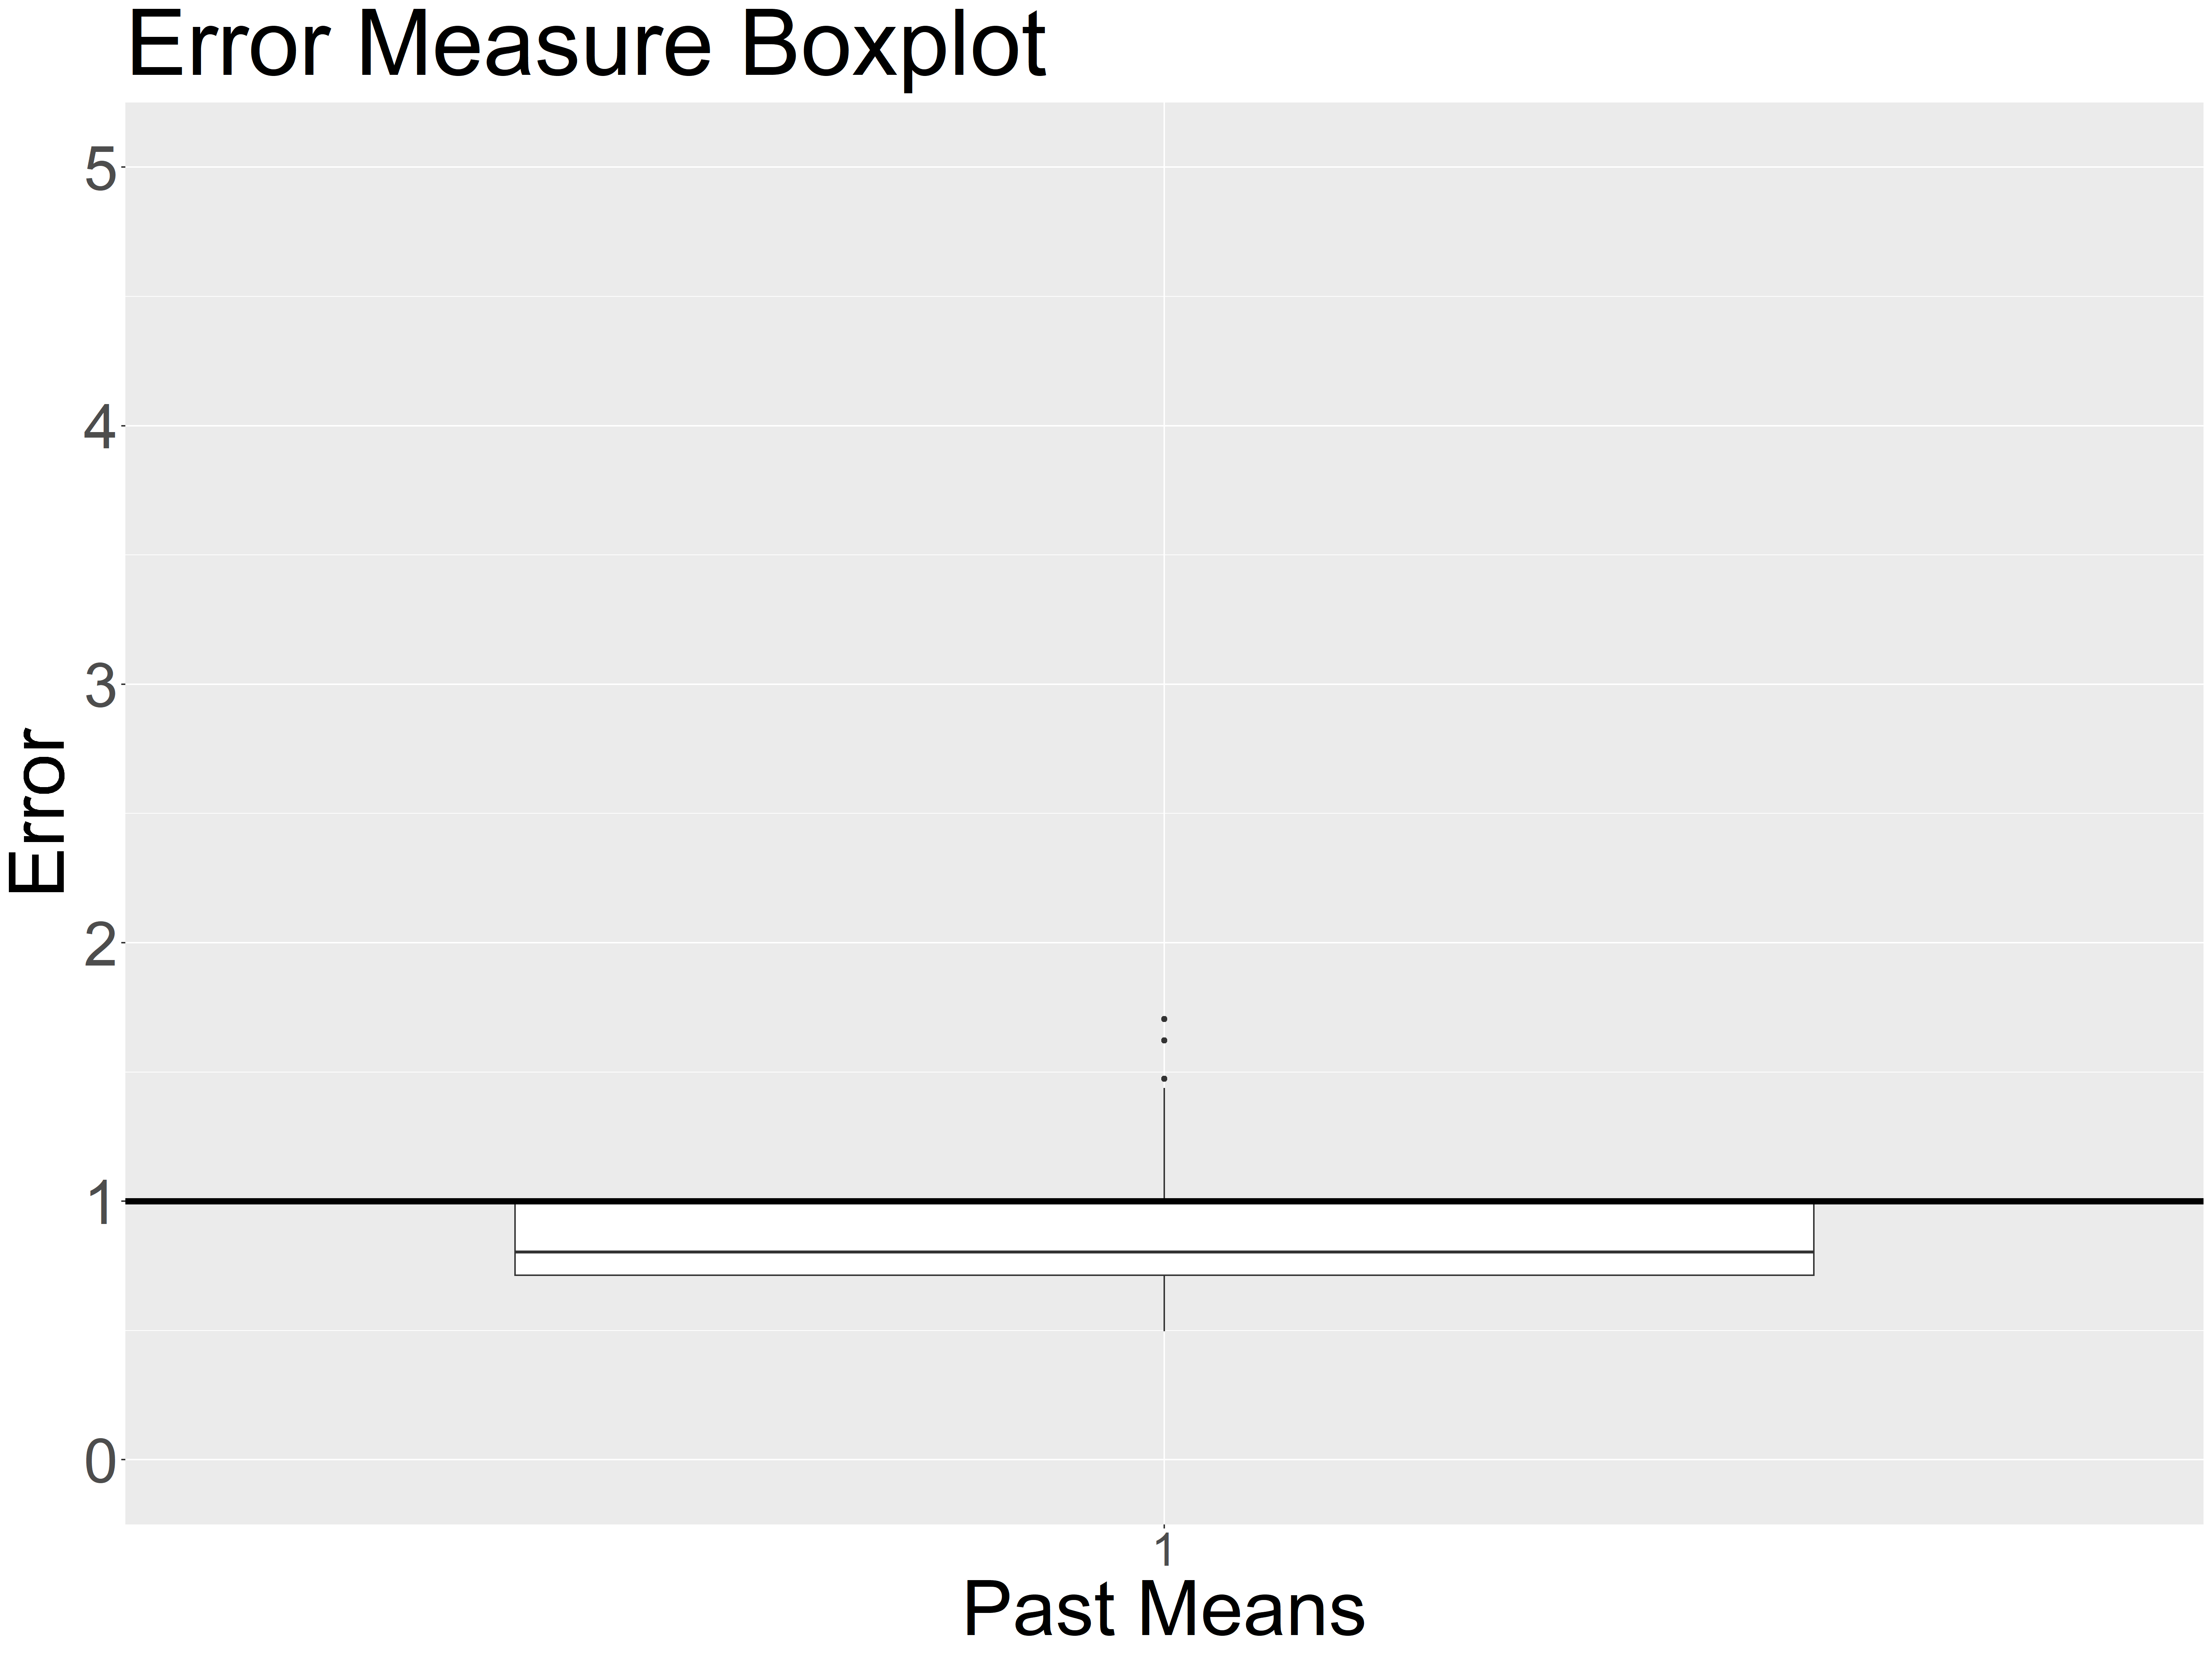
\includegraphics[width=\textwidth]{ErrorMeasureINGARCH_Box_all__Variation_pastOb.png}
\caption{Boxplot for a different number of past observations}
\label{fig:past obs Box}
\end{subfigure}
\hfill
\begin{subfigure}[b]{0.45\textwidth}
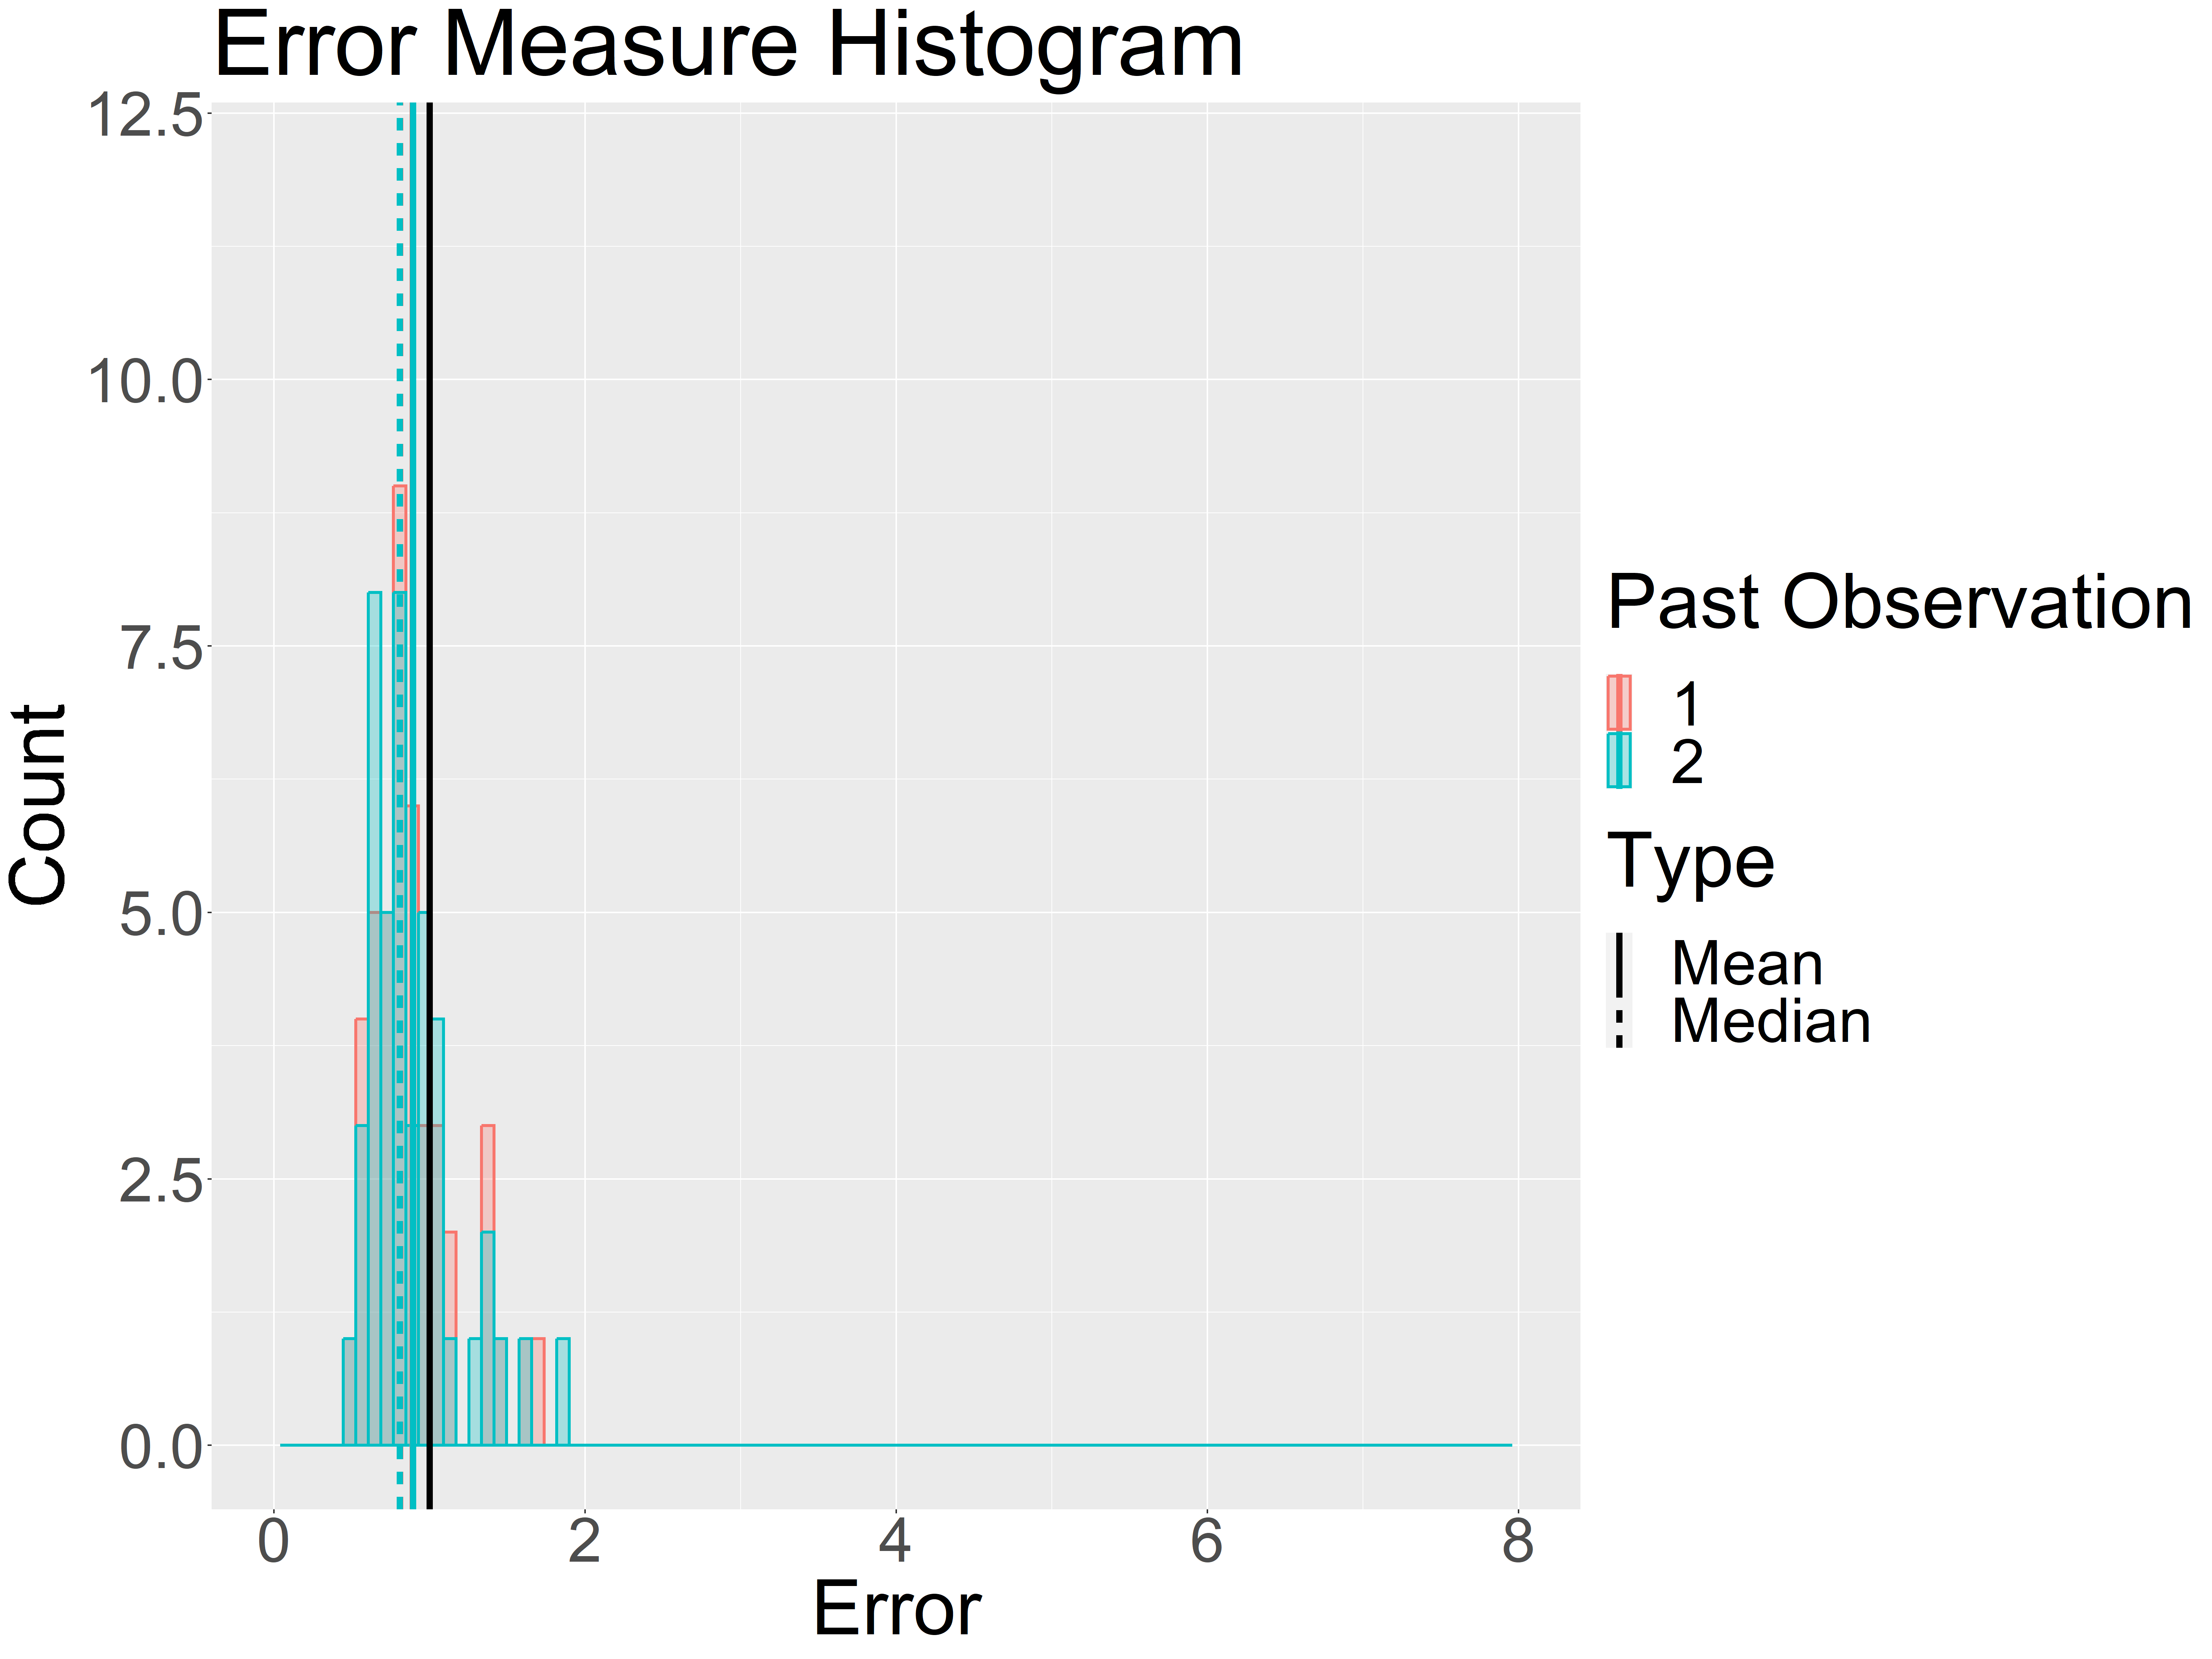
\includegraphics[width=\textwidth]{ErrorMeasureINGARCH_Histogram_all__Variation_pastOb.png}
\caption{Histogram for a different number of past observations}
\label{fig:past obs Hist}
\end{subfigure}
\hfill
\begin{subfigure}[b]{0.8\textwidth}
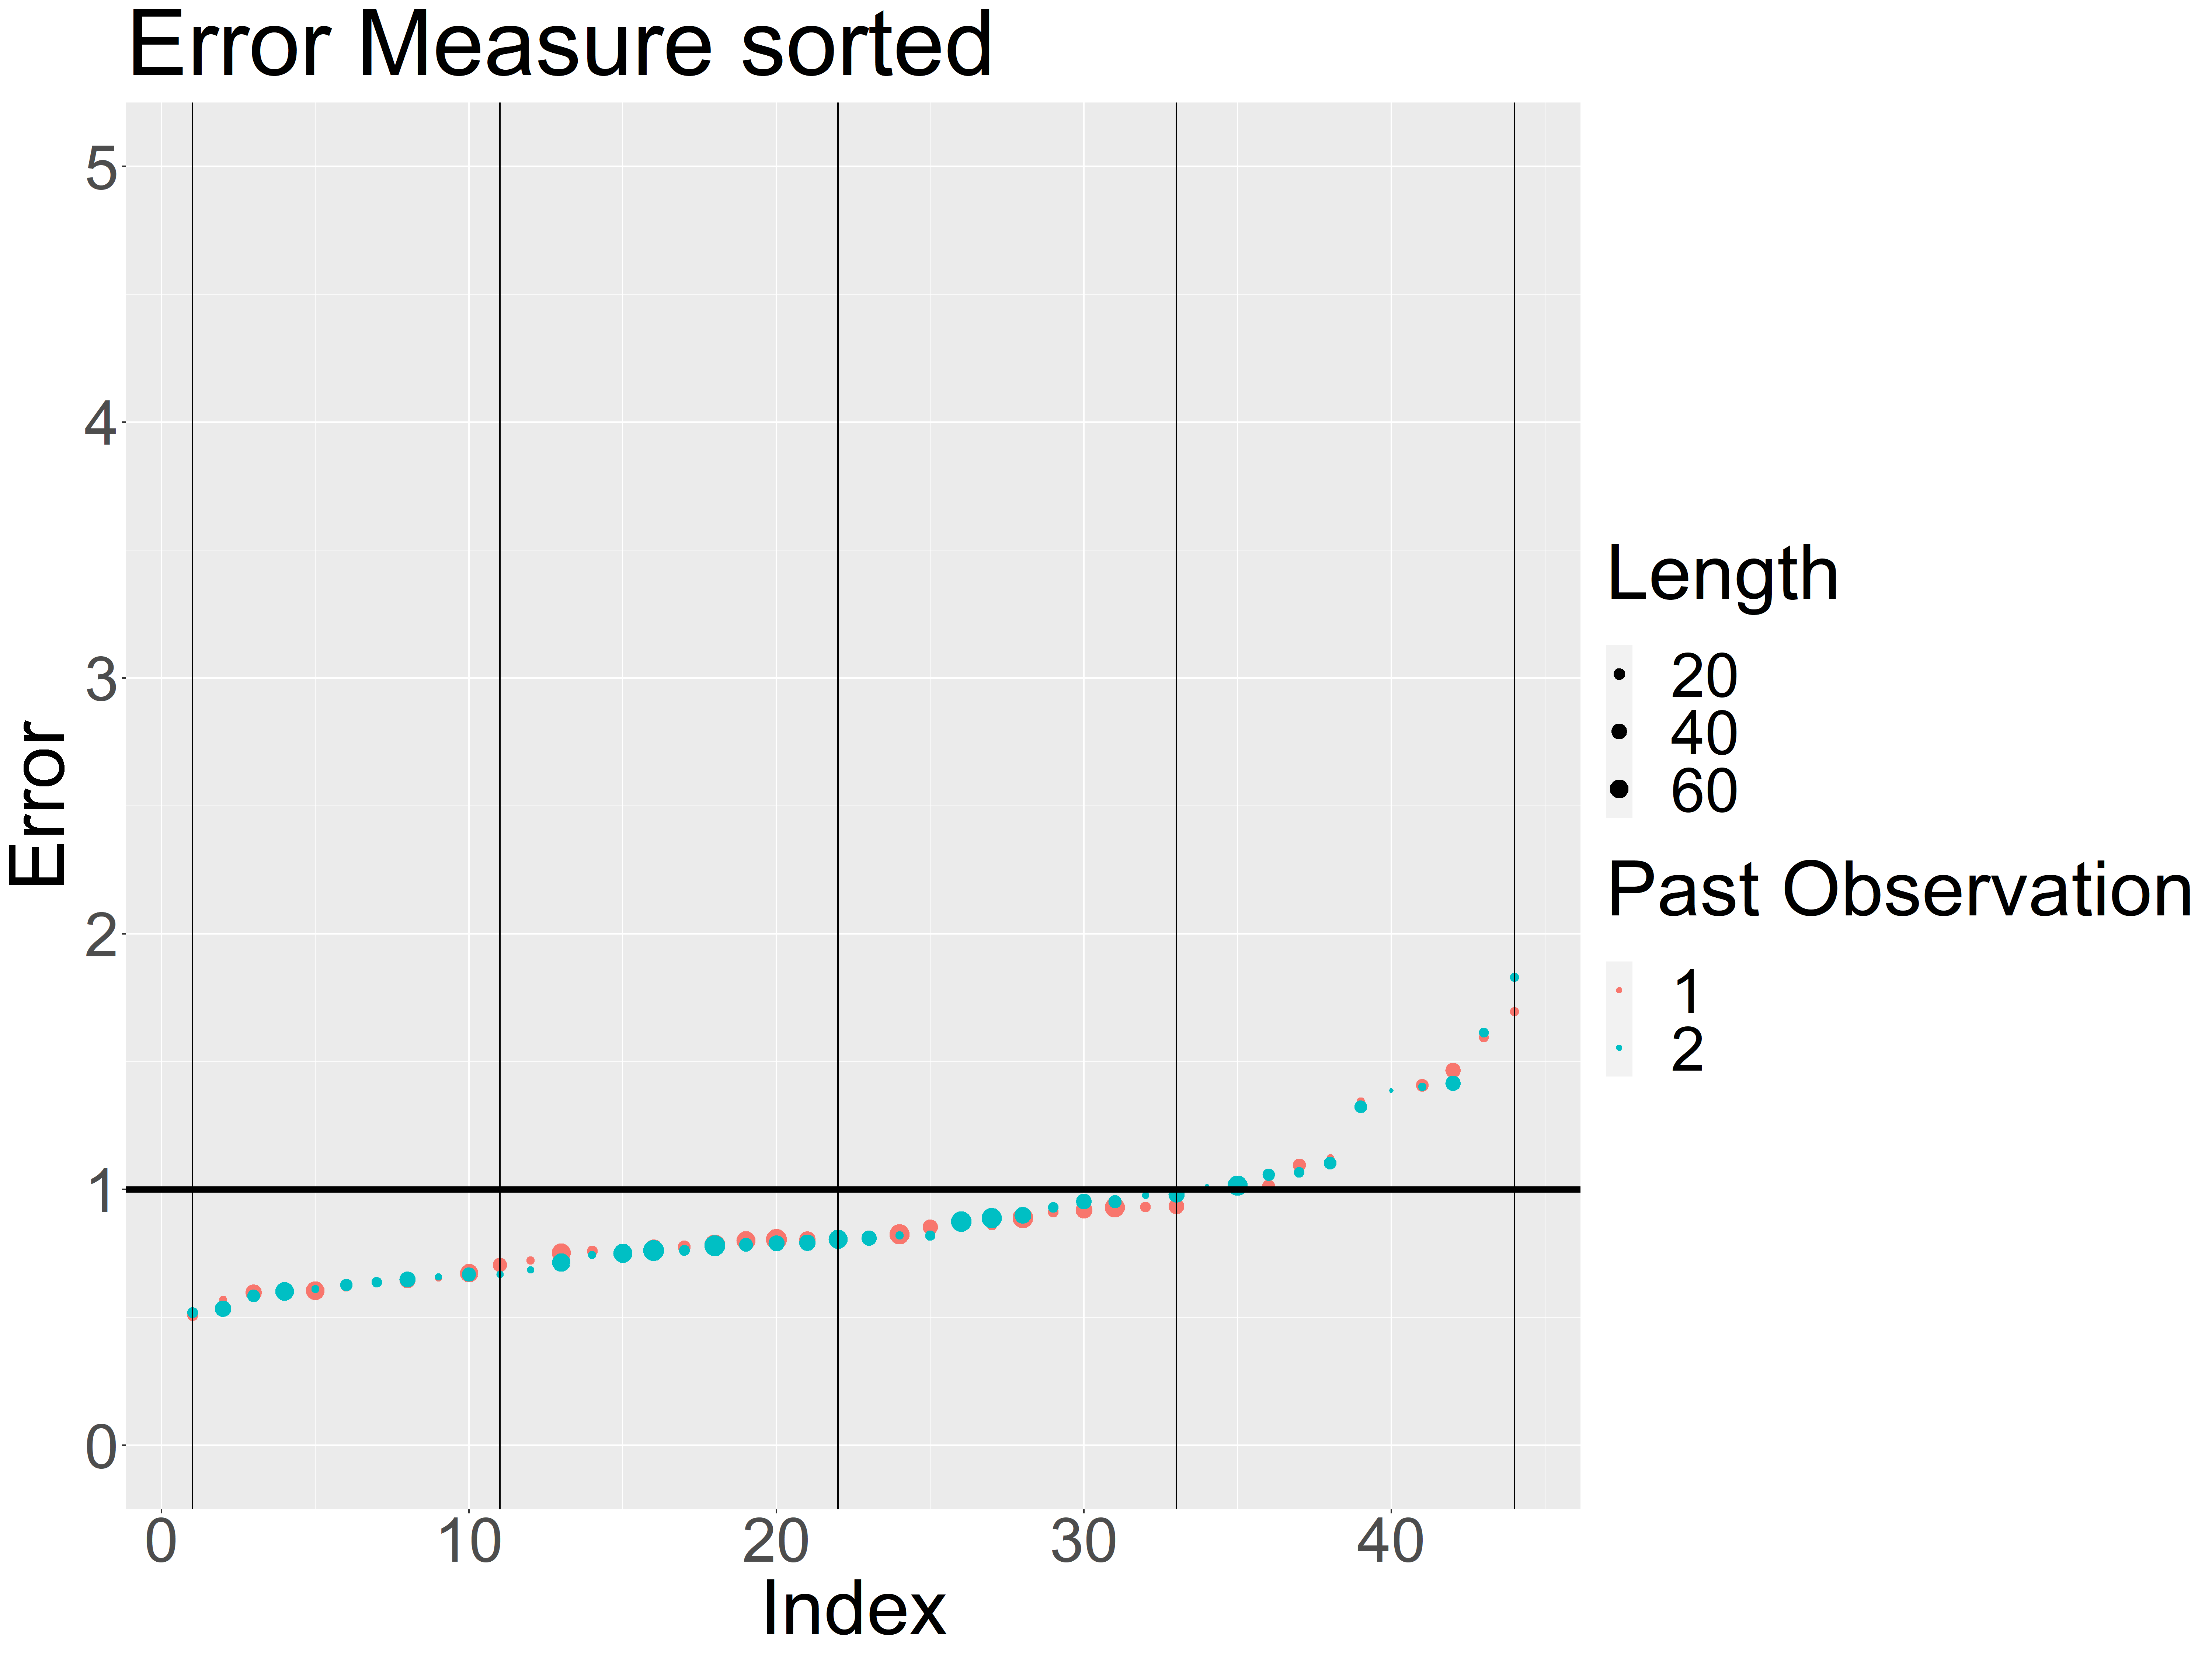
\includegraphics[width=\textwidth]{ErrorMeasureINGARCH_Quant_all__Variation_pastOb.png}
\caption{Quantiles for a different number of past observations}
\label{fig:past obs Quant}
\end{subfigure}
\caption{Comparison of a different number of past observations}
\label{fig:past obs Comp1}
\end{figure}

As we saw, there is not much difference between the INGARCH(1,1), INGARCH(2,1) and INGARCH(1,2) model. One could compare the AIC or some other measure for the different models and base their choice on that. However, this is not further explored here and hence the INGARCH(1,1) model is taken because it is the smallest.

\subsection{CoDA Specifications Results}
\label{sec: CoDA Specifications Results}

Lastly we will compare different CoDA Specifications as mentioned in \ref{sec: Coda Specifications}. Like above we choose one standard model for comparison and always only change one setting. For CoDA our standard model uses extending windows, the full history $h=1$, an initial window length of $w=0.5$, add the simple replacement strategy, no $\Tsp$-spaces and the one-vs-all method. 

\subsection{Zero Handling}
\label{sec: Zero Handling}

First we compare the different options of handling zeros as explained in \ref{sec: Coda Specifications}. The results are shown in figure \ref{fig:Coda zero handling Comp1}. It seems that the simple replacement strategy with $\delta_j = 0.5$, $\forall j$ results in marginally better performance.

\begin{figure}[htb!]
\centering
\begin{subfigure}[b]{0.45\textwidth}
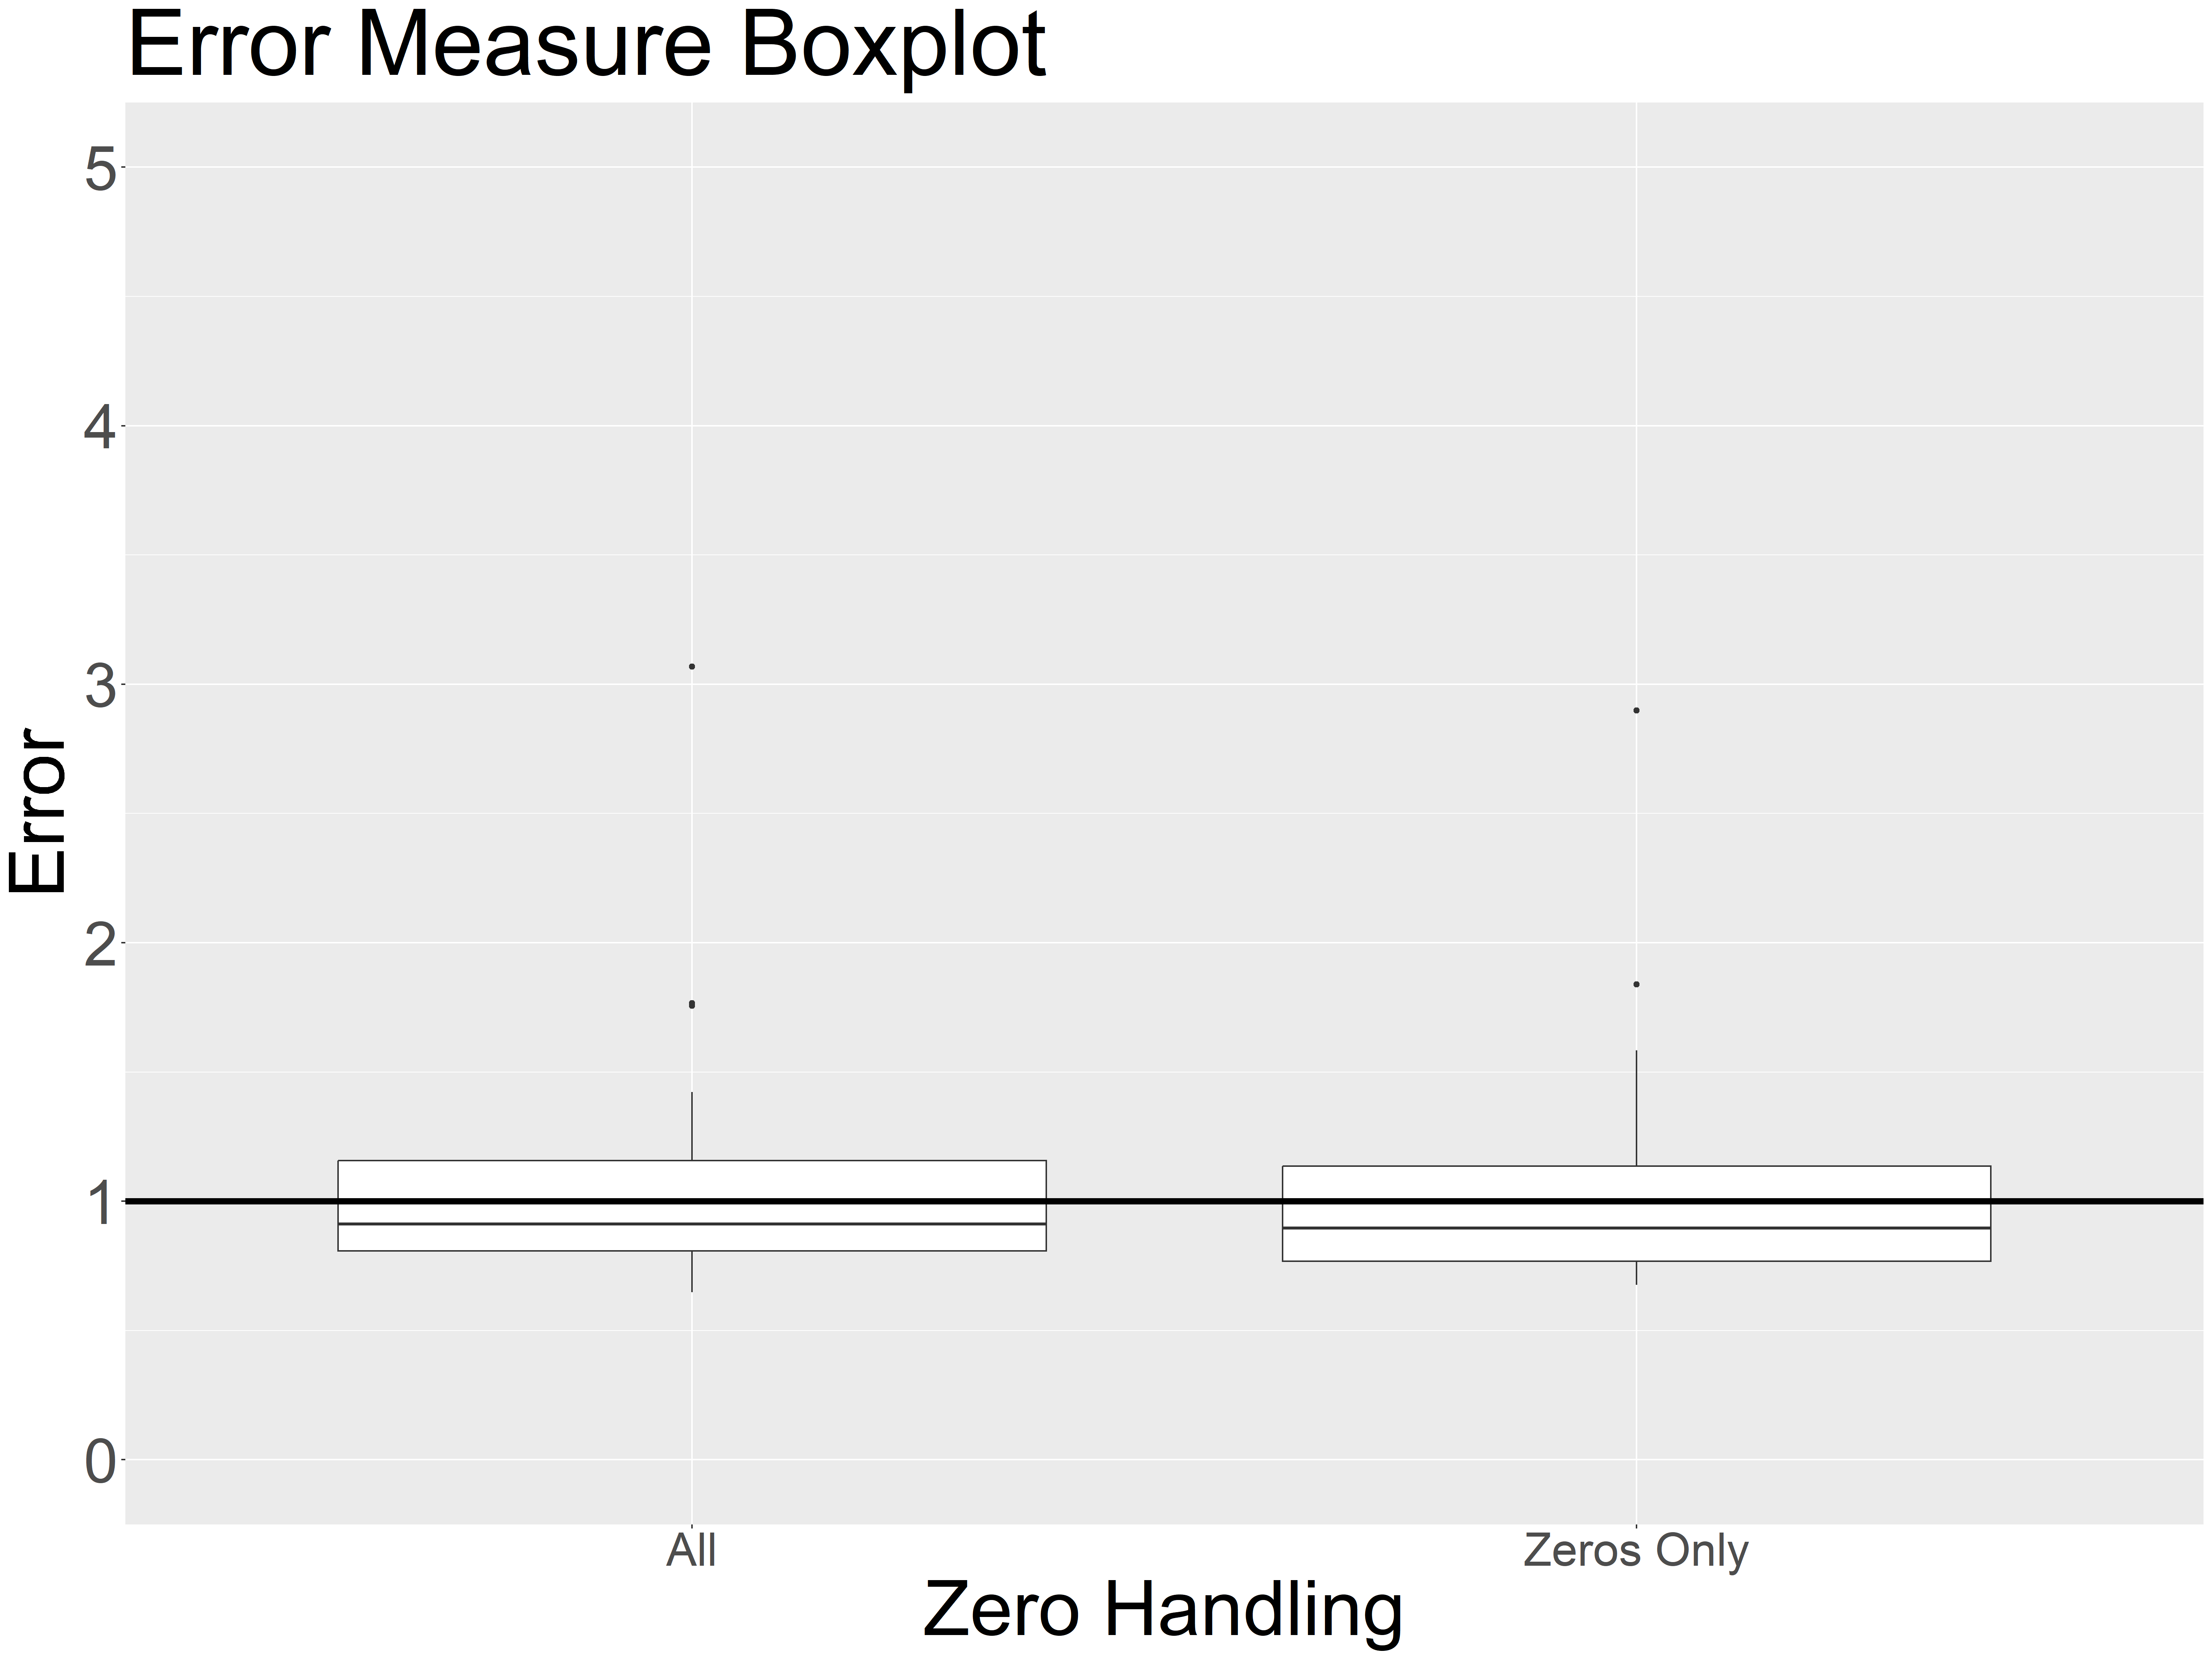
\includegraphics[width=\textwidth]{ErrorMeasureCoDA_Box_all__Variation_zeroHandling.png}
\caption{Boxplot for a different methods of zero handling}
\label{fig:Coda zero handling Box}
\end{subfigure}
\hfill
\begin{subfigure}[b]{0.45\textwidth}
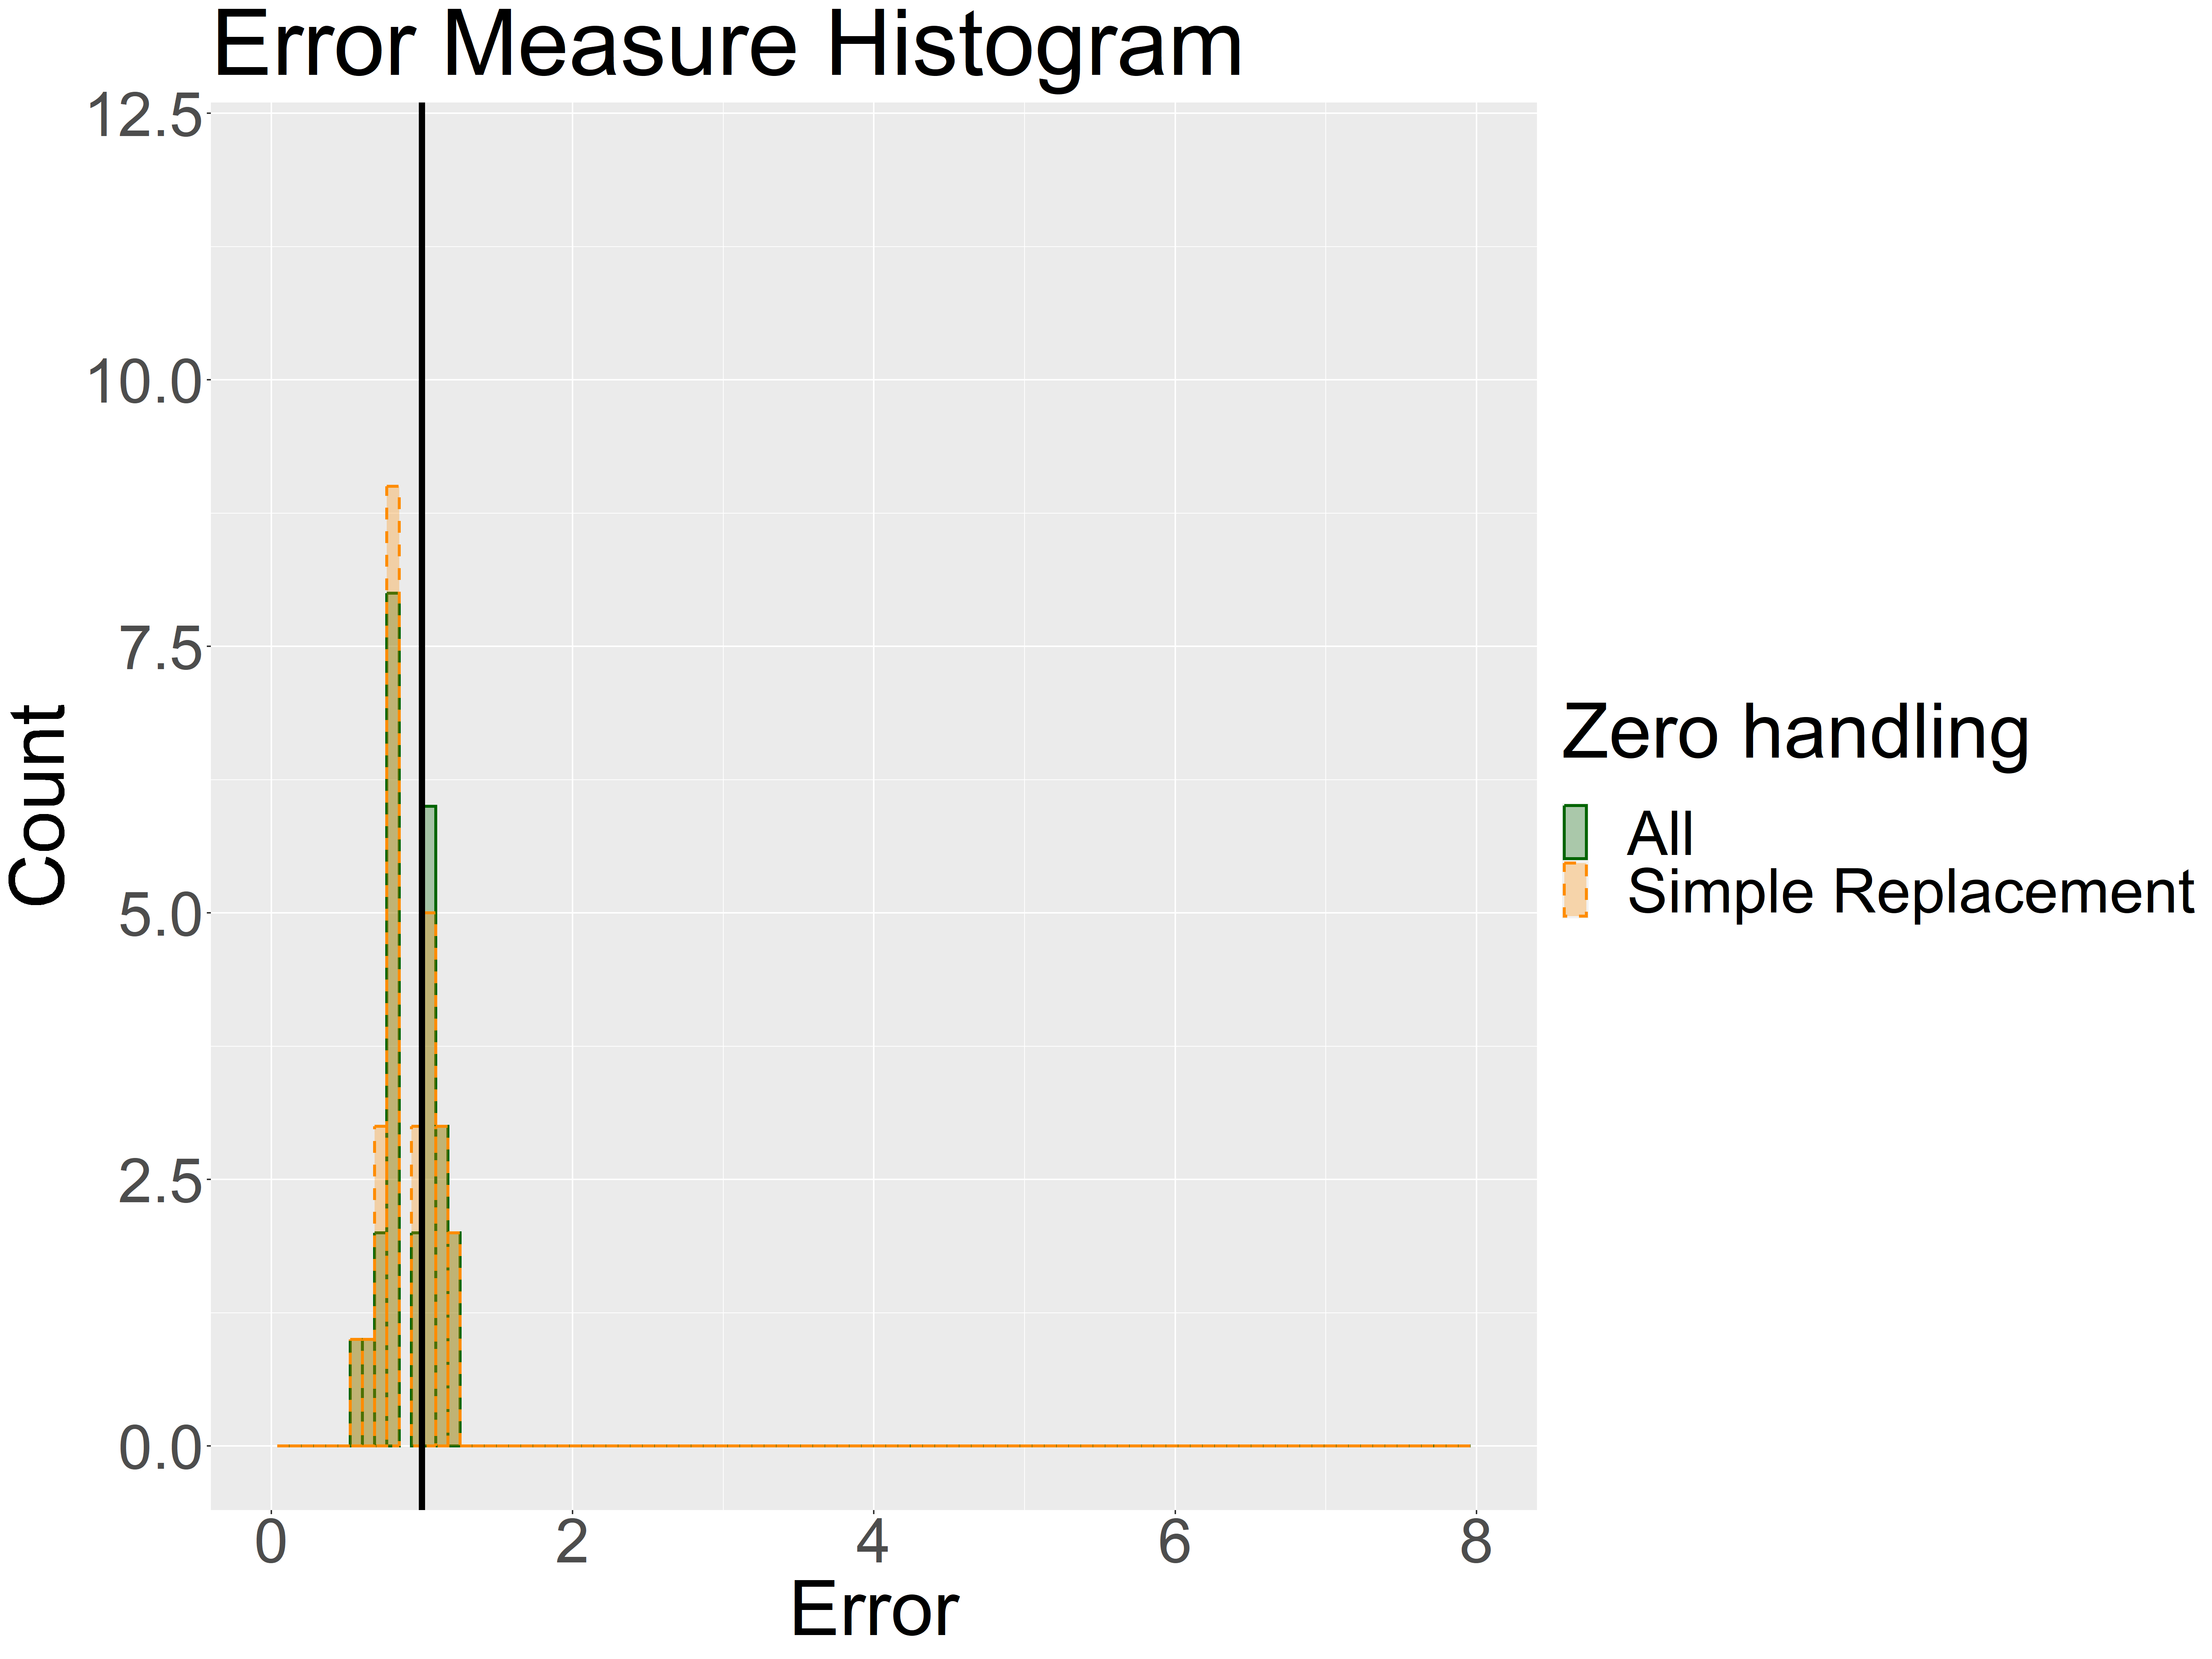
\includegraphics[width=\textwidth]{ErrorMeasureCoDA_Histogram_all__Variation_zeroHandling.png}
\caption{Histogram for a different methods of zero handling}
\label{fig:Coda zero handling Hist}
\end{subfigure}
\hfill
\begin{subfigure}[b]{0.8\textwidth}
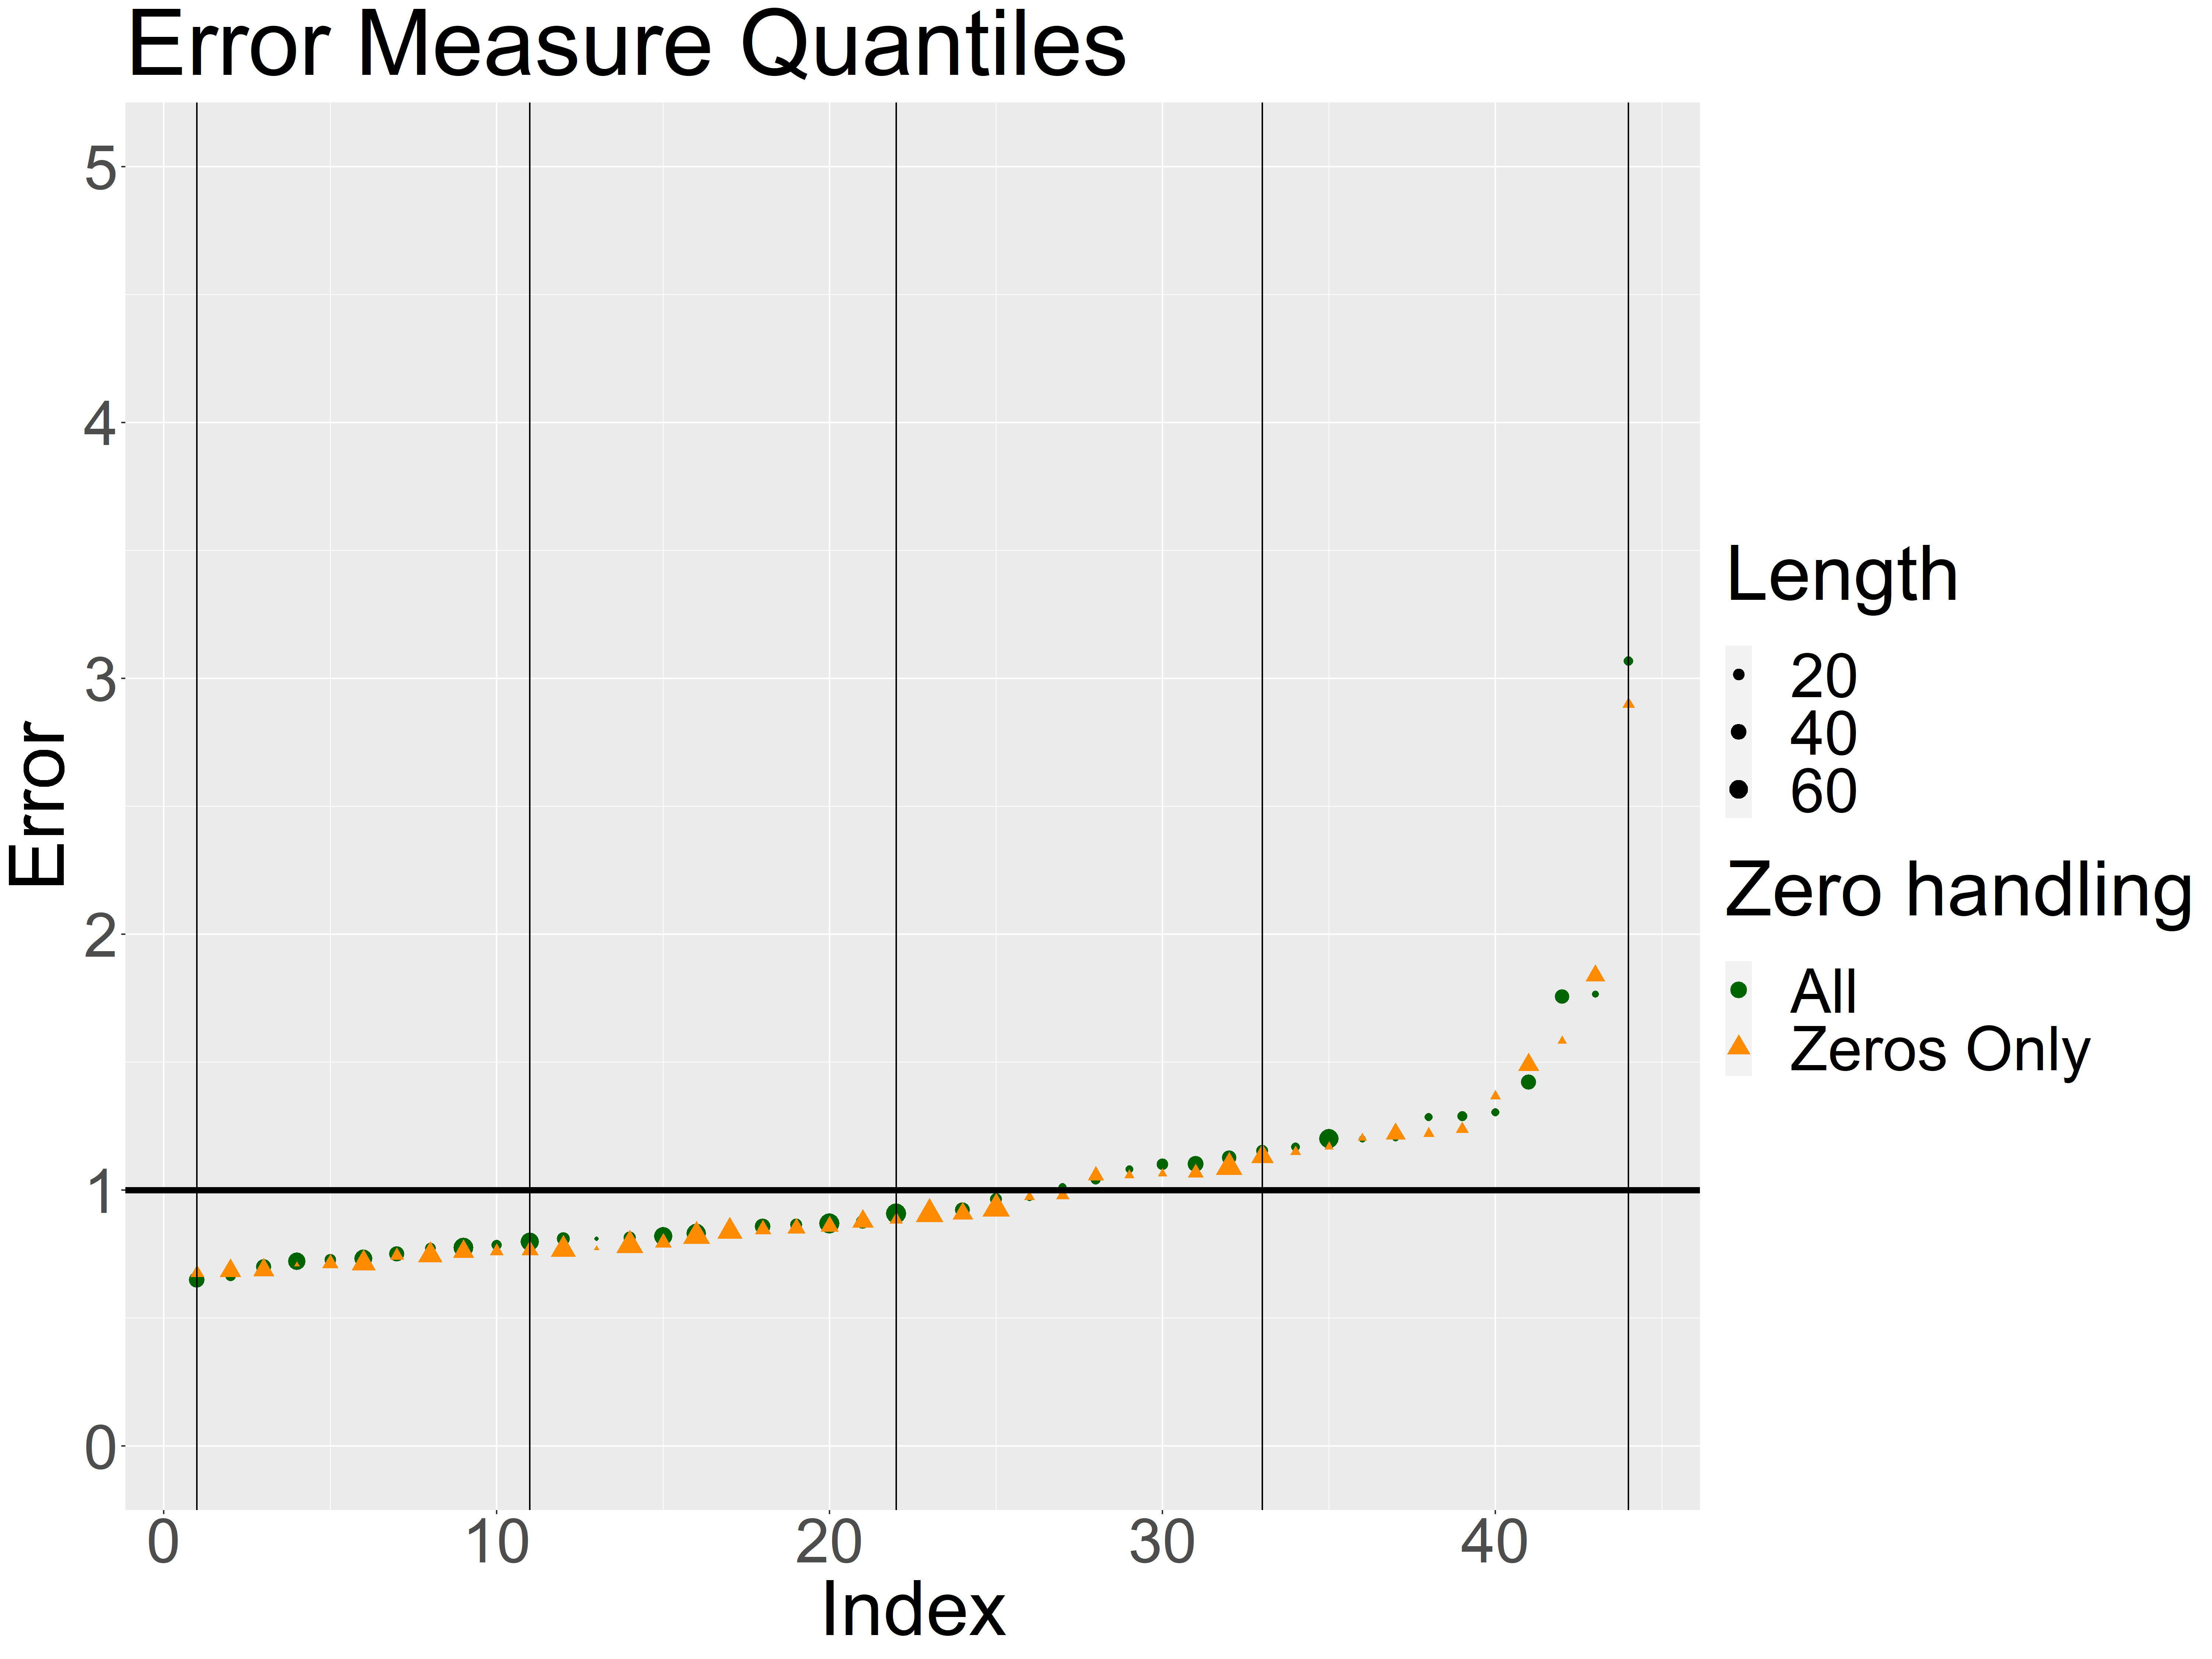
\includegraphics[width=\textwidth]{ErrorMeasureCoDA_Quant_all__Variation_zeroHandling.png}
\caption{Quantiles for a different methods of zero handling}
\label{fig:Coda zero handling Quant}
\end{subfigure}
\caption{Comparison of different zero handling methods}
\label{fig:Coda zero handling Comp1}
\end{figure}


\subsection{$\Tsp$-spaces}
\label{sec: Tspaces results}

Next we compare CoDA for $\Tsp-$Spaces. The results are shown in \ref{fig:Coda T-Spaces Comp1}. It seems that using no $\Tsp-$Spaces result in slightly better results. Especially for shorter time series using no $\Tsp-$Spaces returns better results. This can be seen in figure \ref{fig:Coda T-Spaces Quant}

\begin{figure}[htb!]
\centering
\begin{subfigure}[b]{0.45\textwidth}
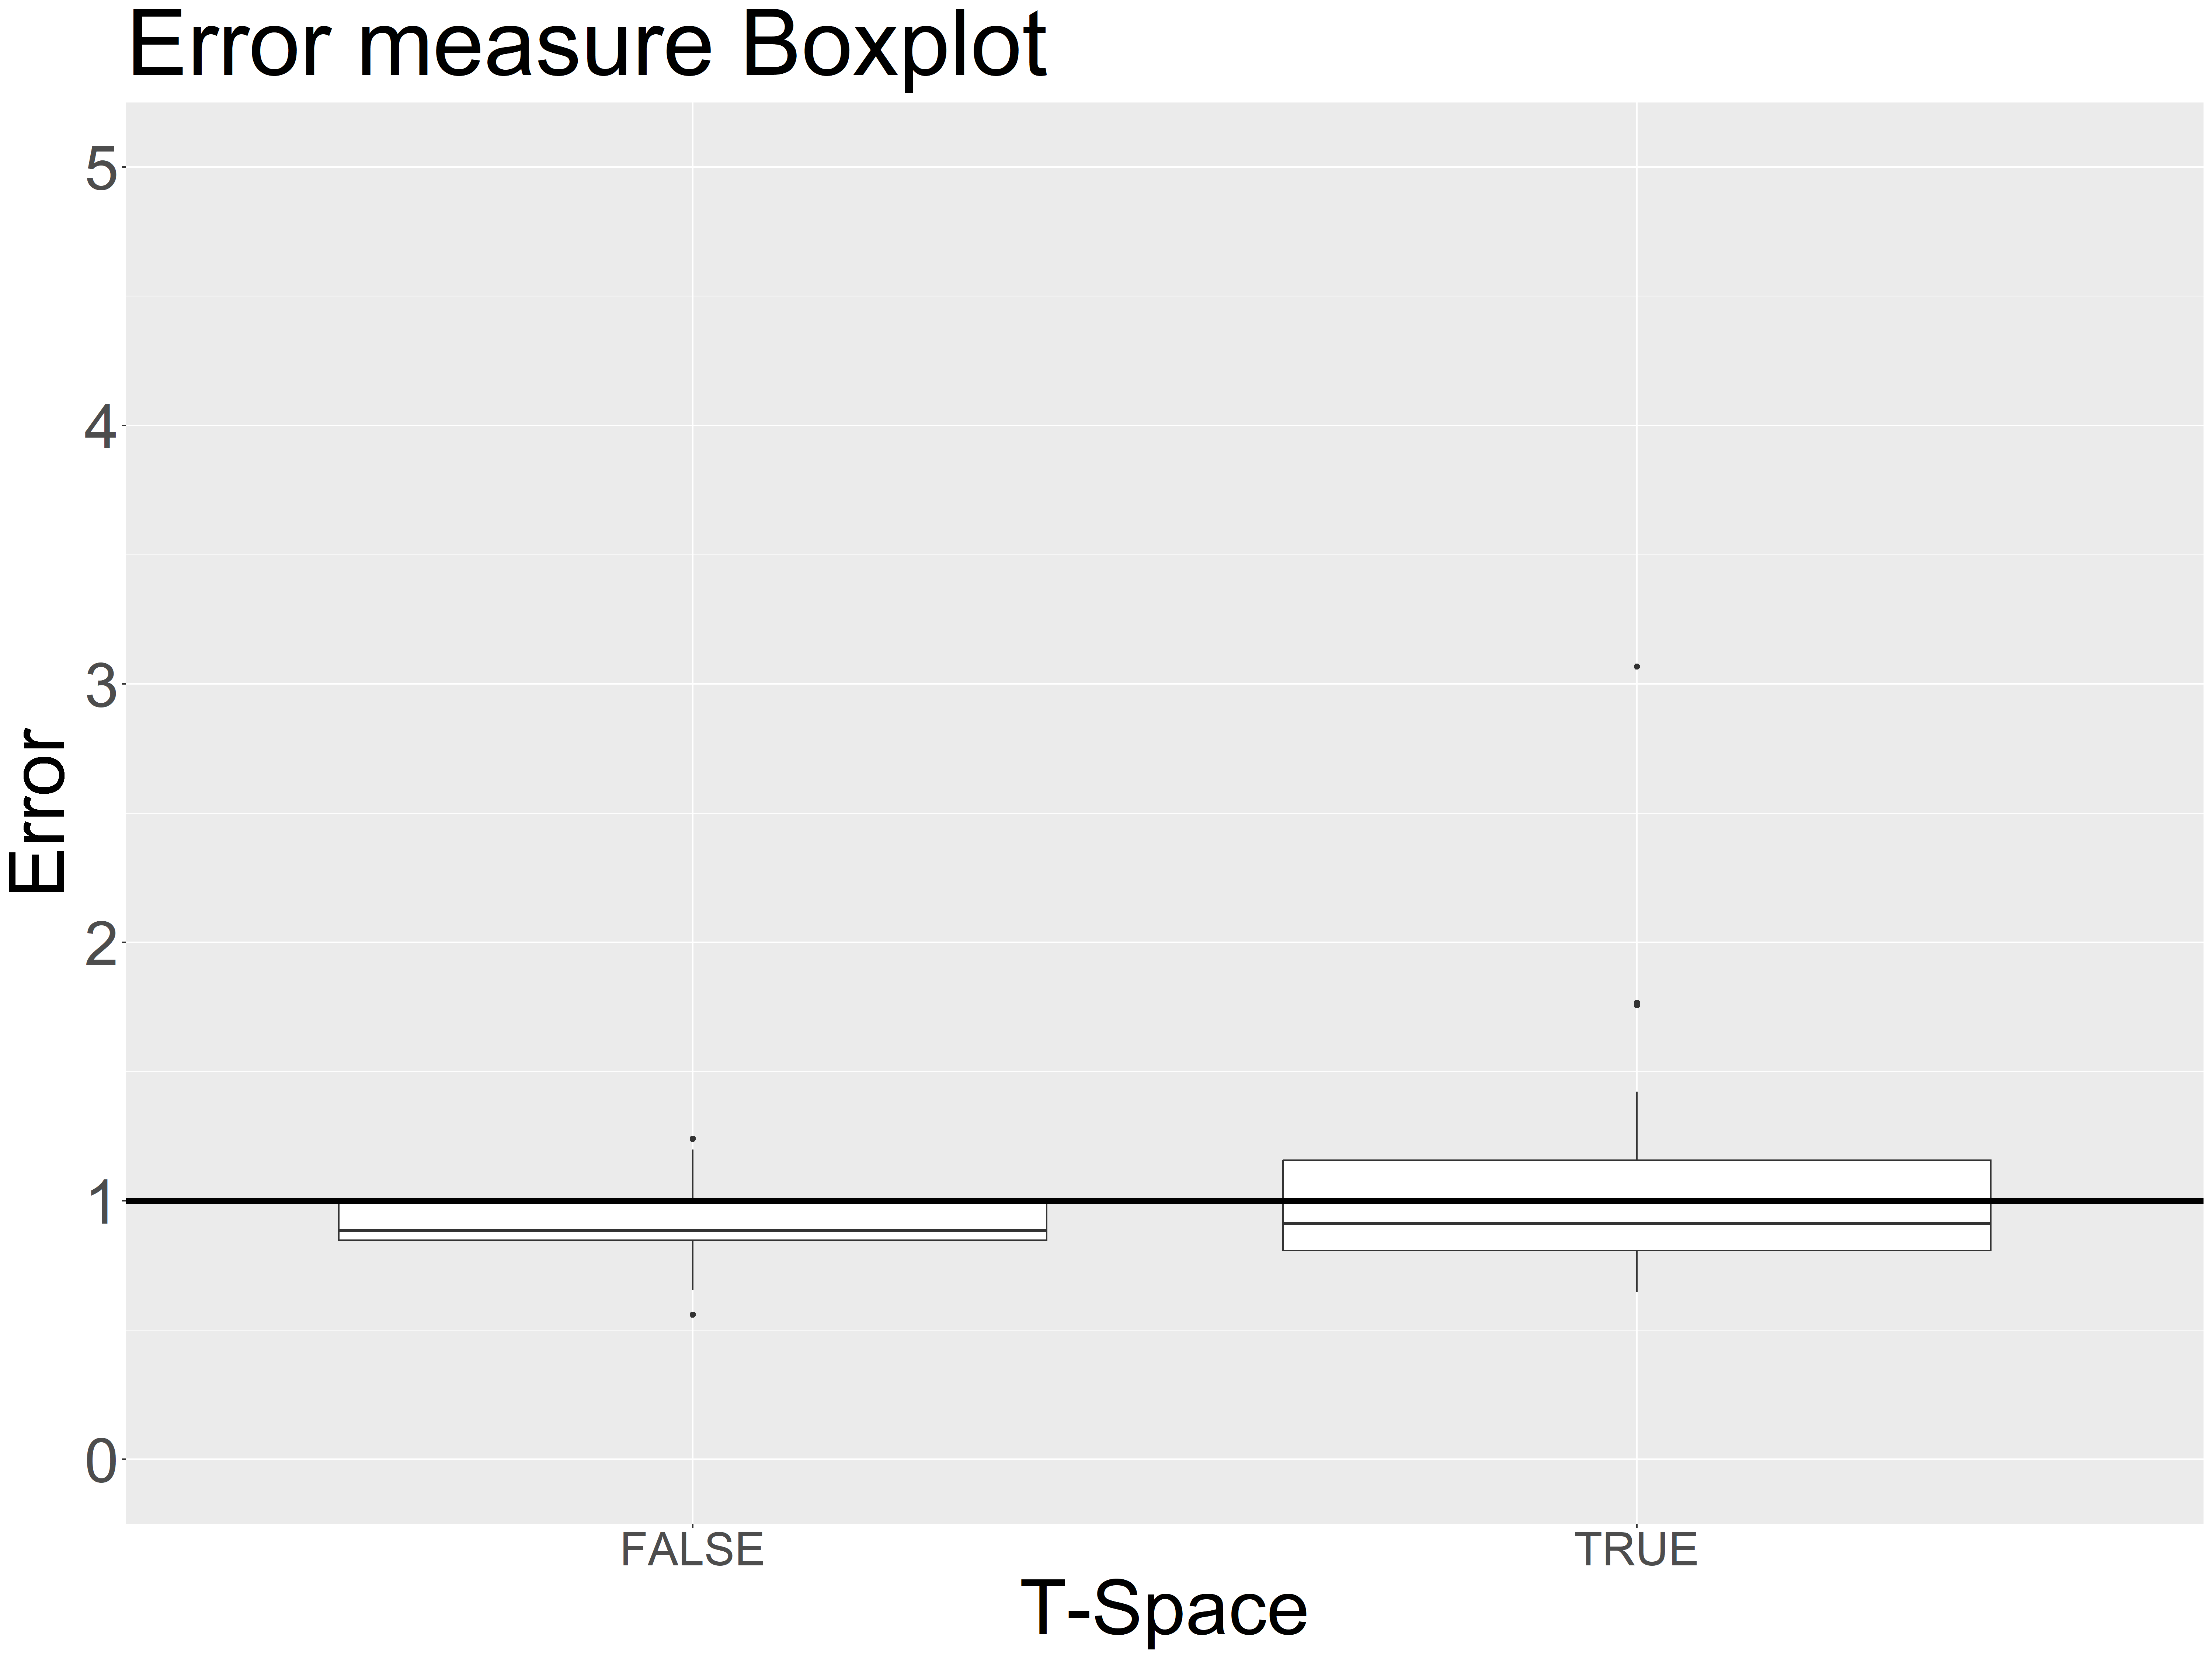
\includegraphics[width=\textwidth]{ErrorMeasureCoDA_Box_all__Variation_tSpace.png}
\caption{Boxplot for $\Tsp-$Spaces}
\label{fig:Coda T-Spaces Box}
\end{subfigure}
\hfill
\begin{subfigure}[b]{0.45\textwidth}
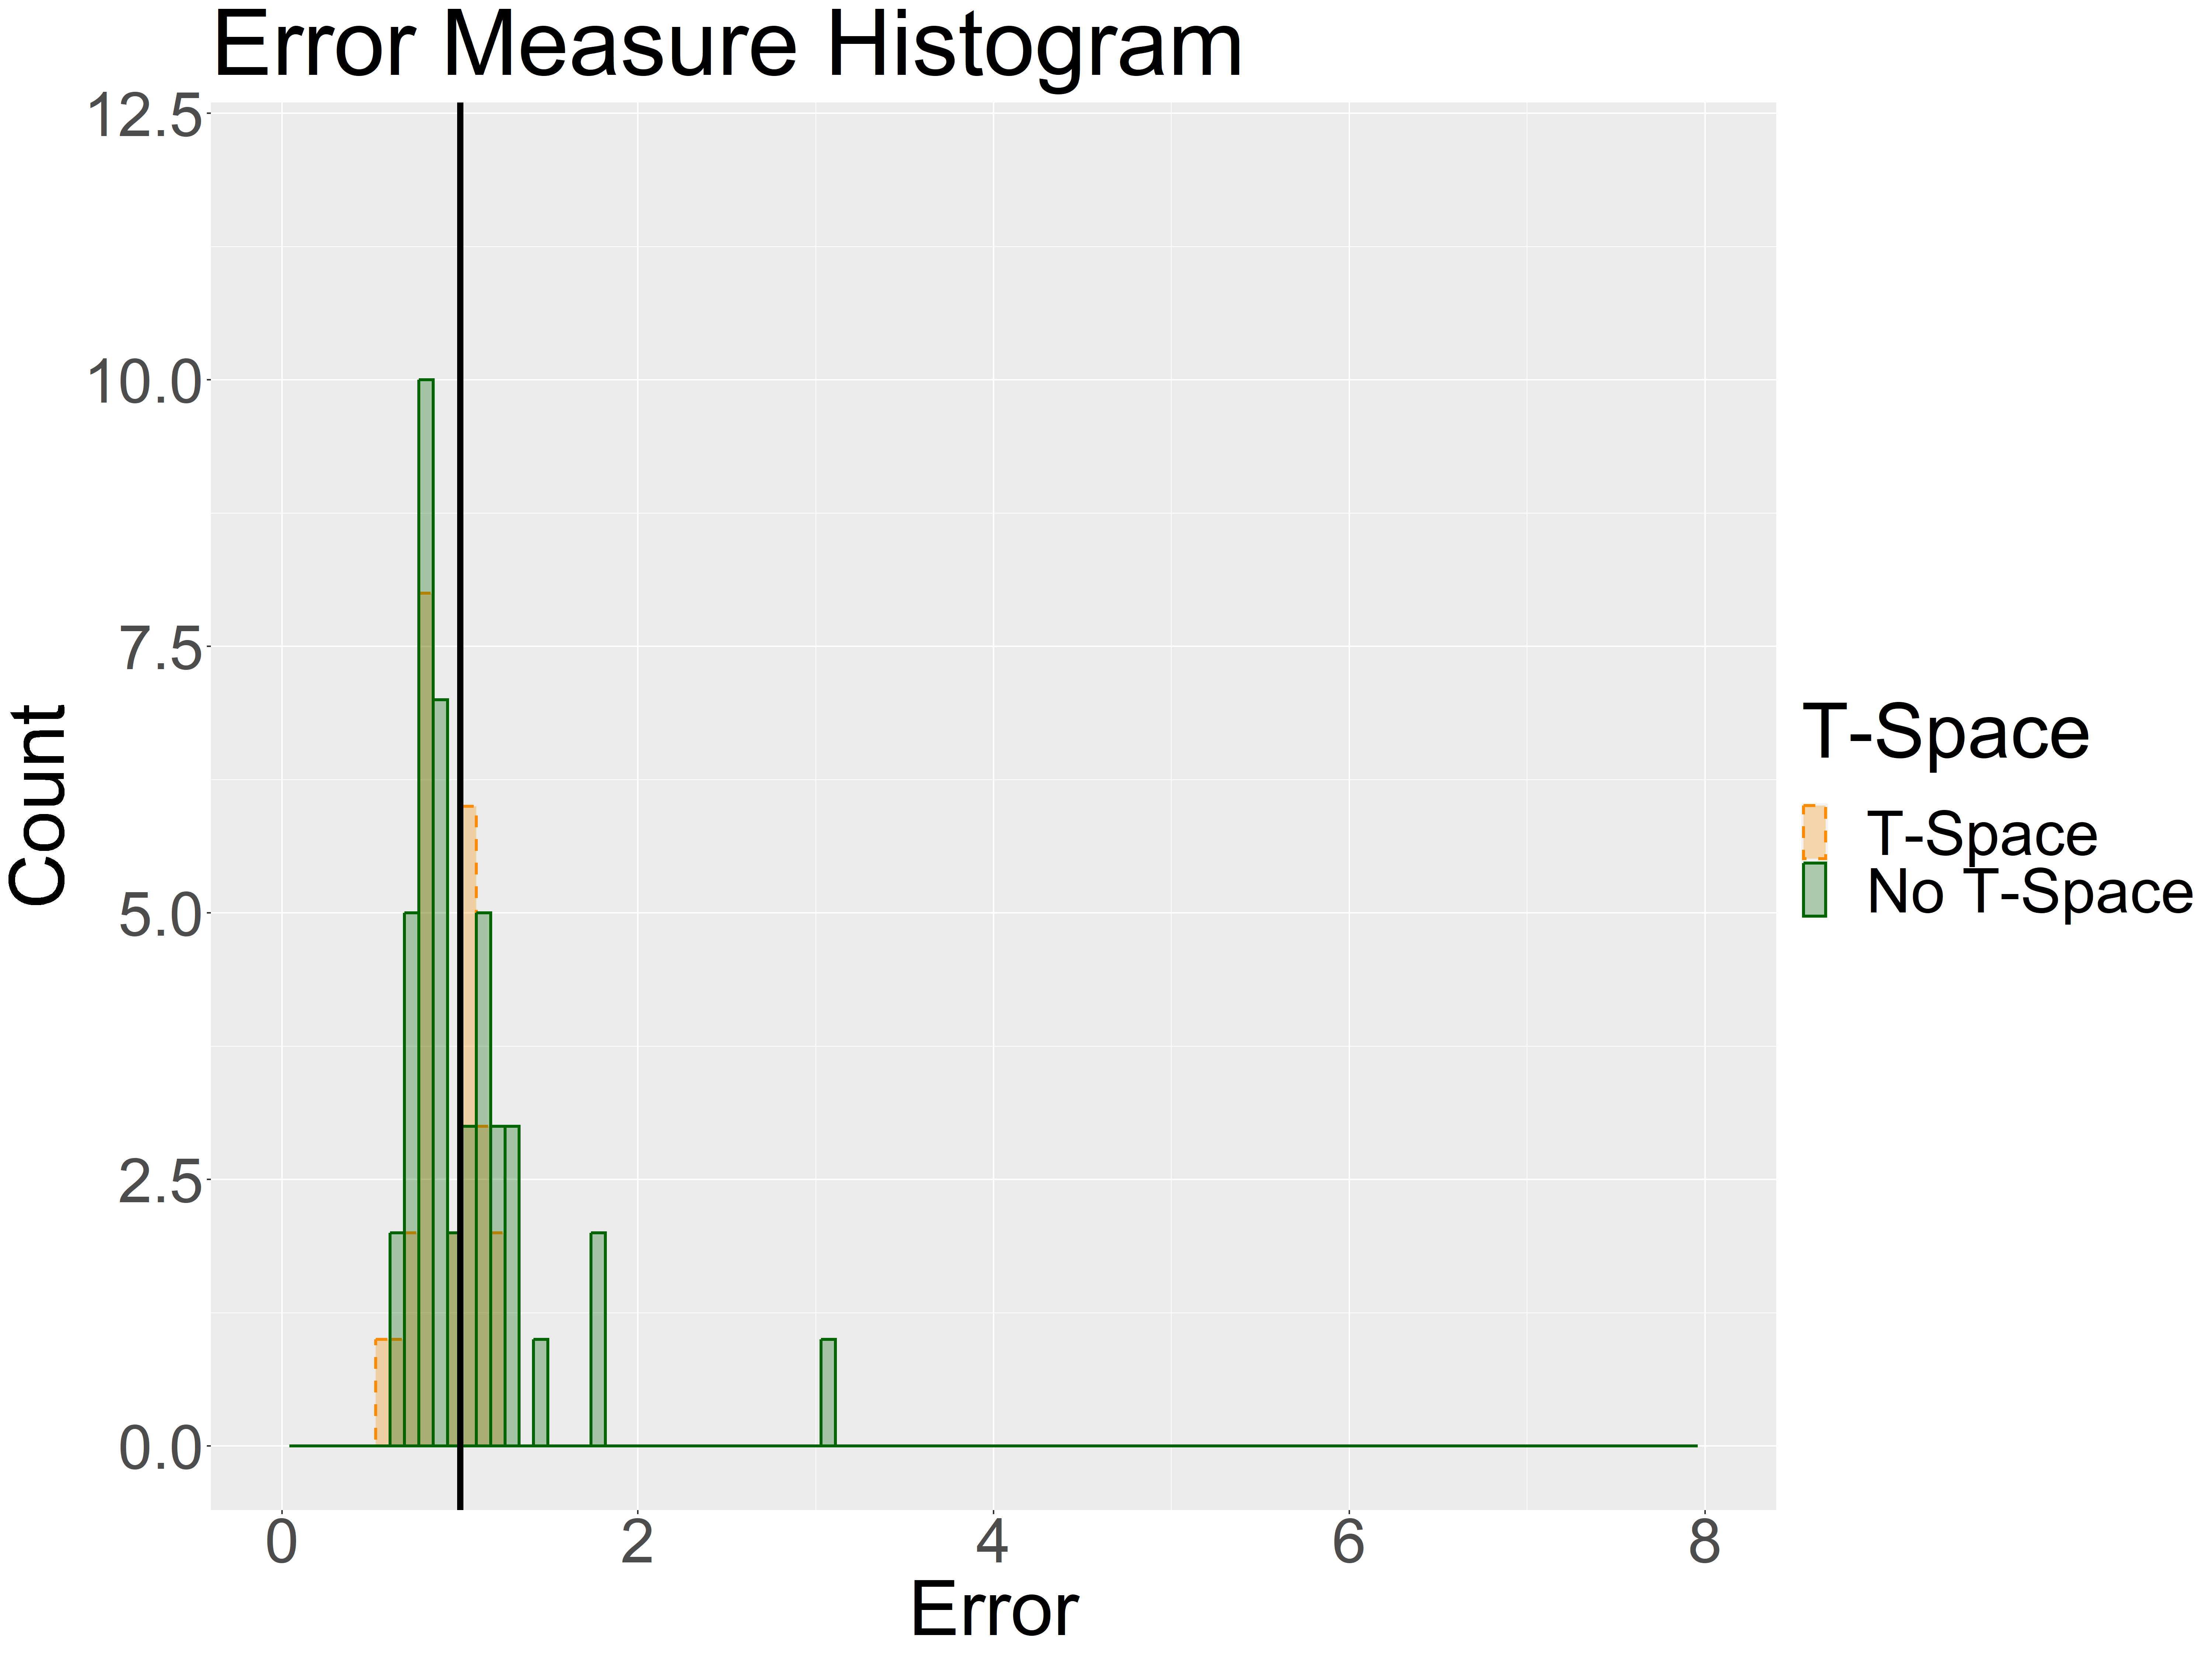
\includegraphics[width=\textwidth]{ErrorMeasureCoDA_Histogram_all__Variation_tSpace.png}
\caption{Histogram for $\Tsp-$Spaces}
\label{fig:Coda T-Spaces Hist}
\end{subfigure}
\hfill
\begin{subfigure}[b]{0.8\textwidth}
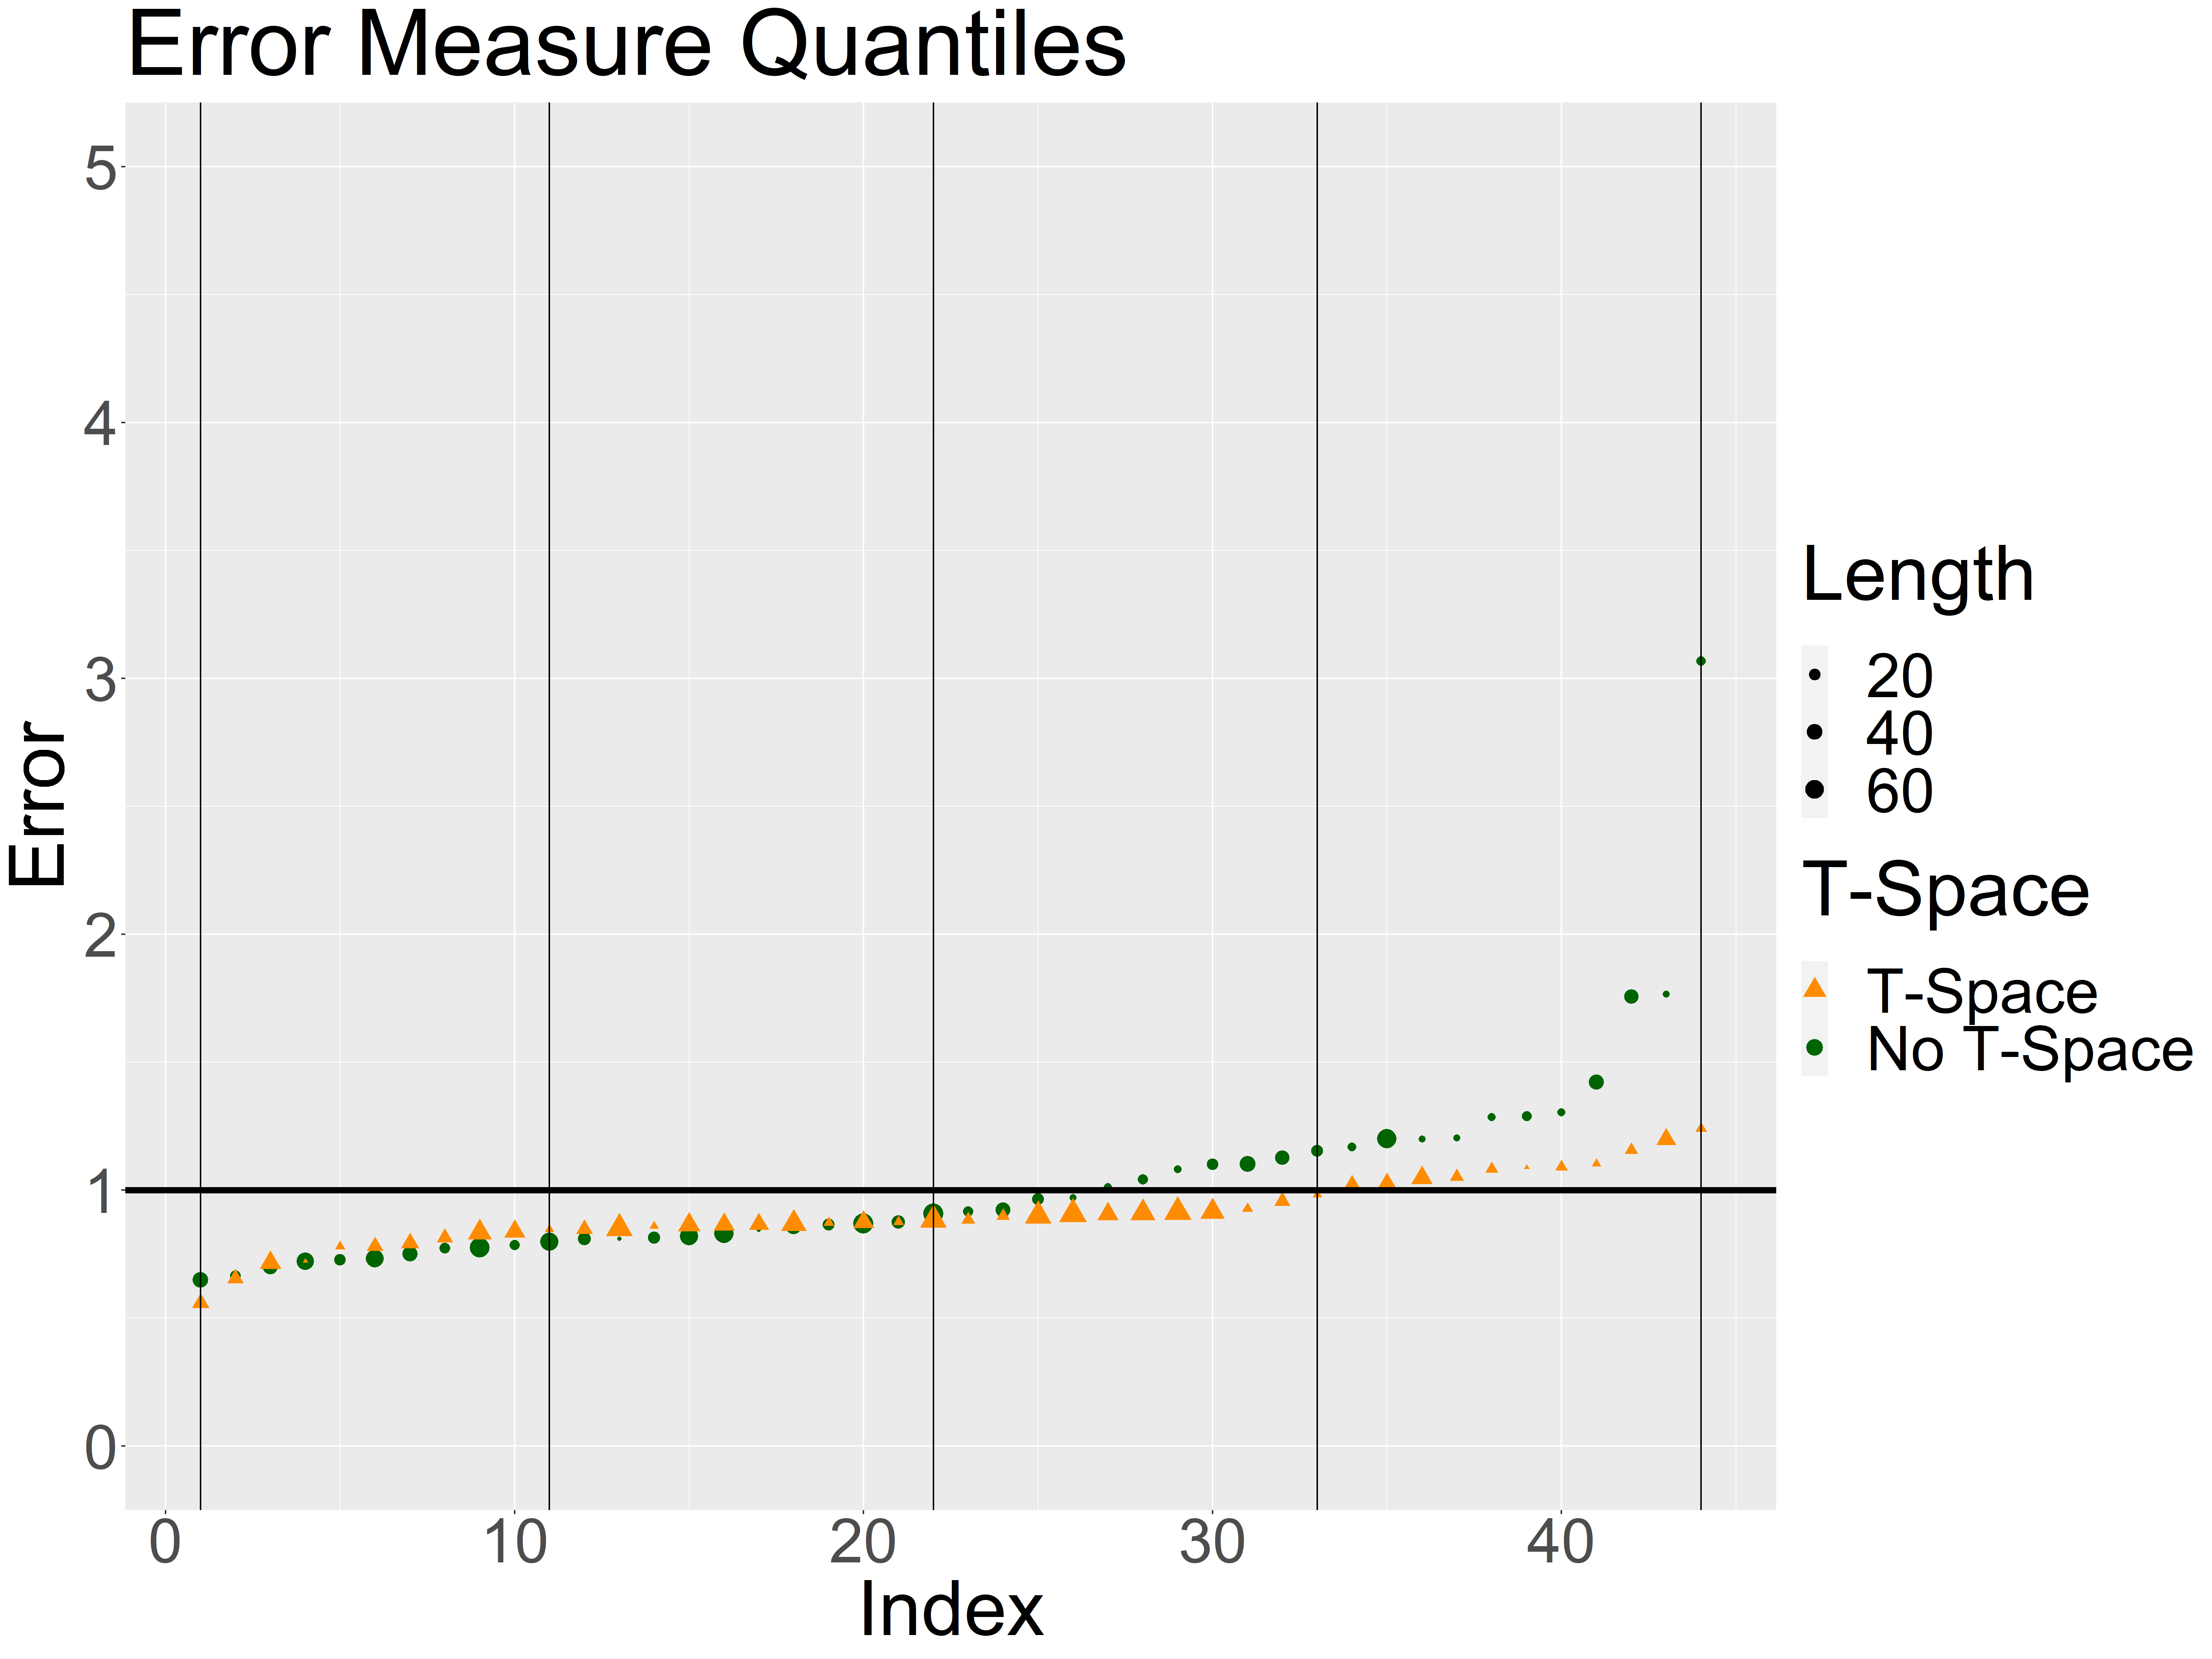
\includegraphics[width=\textwidth]{ErrorMeasureCoDA_Quant_all__Variation_tSpace.png}
\caption{Quantiles for $\Tsp-$Spaces}
\label{fig:Coda T-Spaces Quant}
\end{subfigure}
\caption{Comparison of CoDA with and without $\Tsp-$Spaces}
\label{fig:Coda T-Spaces Comp1}
\end{figure}


\subsection{One-vs-All method}
\label{sec: One-vs-All}

Now we analyse the one-vs-all method. Figure \ref{fig:Coda One-vs-All Comp1} shows the results. We can clearly seen, that the one-vs-all method performs better over all time series. This difference is highlighted in figure \ref{fig:Coda One-vs-All Quant}. 

\begin{figure}[htb!]
\centering
\begin{subfigure}[b]{0.45\textwidth}
\includegraphics[width=\textwidth]{ErrorMeasureCoDA_Box_all__Variation_oneVSAll.png}
\caption{Boxplot for One-vs-All}
\label{fig:Coda One-vs-All Box}
\end{subfigure}
\hfill
\begin{subfigure}[b]{0.45\textwidth}
\includegraphics[width=\textwidth]{ErrorMeasureCoDA_Histogram_all__Variation_oneVSAll.png}
\caption{Histogram for One-vs-All}
\label{fig:Coda One-vs-All Hist}
\end{subfigure}
\hfill
\begin{subfigure}[b]{0.8\textwidth}
\includegraphics[width=\textwidth]{ErrorMeasureCoDA_Quant_all__Variation_oneVSAll.png}
\caption{Quantiles for One-vs-All}
\label{fig:Coda One-vs-All Quant}
\end{subfigure}
\caption{Comparison of CoDA with and without One-vs-All}
\label{fig:Coda One-vs-All Comp1}
\end{figure}

















